\documentclass[bibliography=totoc, abstract=on]{scrartcl}

\usepackage{fancyhdr}
\fancyhead{}
\fancyfoot{}
\fancyhead[RO,RE]{\slshape \leftmark}
\fancyhead[LO,LE]{\slshape \rightmark}
\fancyfoot[C]{\thepage}

\setlength{\columnsep}{25pt}
\setlength{\columnseprule}{0.4pt}

\renewcommand{\contentsname}{Table of Contents}

\usepackage[format=plain, labelfont=bf, textfont=it, margin=1cm]{caption}
\usepackage[utf8]{inputenc}
\usepackage{graphicx}
\usepackage{subcaption}
\usepackage{pdfpages}
\usepackage[colorinlistoftodos]{todonotes}
\usepackage{float}
\usepackage{amsmath}
\usepackage[section=section]{glossaries}
\usepackage{tikz}
\usepackage{icomma}
\usepackage{pgfplots, pgfplotstable}
\usepackage{bchart}
\usepackage{mathtools}
\usepackage{csquotes}
\usepackage{chngcntr}
\usepackage{multirow}
\usepackage{soul}

\usepackage[backend=biber,style=ieee,sortlocale=en_UK,natbib=true,url=true,doi=true,eprint=true,autocite=superscript]{biblatex}

\usetikzlibrary{automata,positioning,patterns}
\pgfplotsset{width=12cm,compat=1.9}

\DeclarePairedDelimiter{\floor}{\lfloor}{\rfloor}
\DeclareOldFontCommand{\sl}{\normalfont}{\mathbf}
\DeclareOldFontCommand{\rm}{\normalfont}{\mathbf}

\usepackage{titlesec}

\addbibresource{appendix/references.bib}
\let\cite\supercite

\makeglossaries
\makeglossaries

\newglossaryentry{Ethereum}
{
    name=Ethereum,
    description={open-source, public, blockchain-based decentralized computing platform}
}
 
\newglossaryentry{Blockchain}
{
    name=blockchain,
    description={continuously growing list of records, called blocks, which are linked and secured using cryptography}
}

\newglossaryentry{cryptocurrency}
{
    name=cryptocurrency,
    description={a digital asset, that is powered by blockchain technology},
    plural={cryptocurrencies}
}

\newglossaryentry{decentralization}
{
    name=decentralization,
    description={distribution of computational and functional resources across the network \textit{(in context of information theory)}}
}

\newglossaryentry{traditional model}
{
    name=traditional model,
    description={system architecture, that uses a central server architecture for data communication and storage \textit{(in context of this thesis work)}}
}

\newglossaryentry{peer-to-peer}
{
    name=peer-to-peer,
    description={distributed application architecture that partitions tasks or workloads between peers}
}

\newglossaryentry{distributed general ledger}
{
    name=distributed general ledger,
    description={consensus of replicated, shared, and synchronized digital data, spread across multiple nodes}
}

\newglossaryentry{open-source}
{
    name=open-source,
    description={software, whose code is made public and which is thus available to any programmer to develop and customize}
}

\newglossaryentry{public blockchain}
{
    name=public blockchain,
    description={a blockchain, where all nodes are allowed to participate in the network, execute the consensus protocol and maintain the general ledger},
    plural={public blockchains}
}

\newglossaryentry{semi-decentralized public blockchain}
{
    name=semi-decentralized public blockchain,
    description={a blockchain, where only a selection of nodes are allowed to execute the consensus protocol and maintain the general ledger},
    plural={semi-decentralized public blockchains}
}

\newglossaryentry{private blockchain}
{
    name=private blockchain,
    description={a blockchain, where nodes can participate in the network only by obtaining a permission from a central organization that is deploying the blockchain},
    plural={private blockchains}
}

\newglossaryentry{client-server}
{
    name=client-server,
    description={see \textbf{traditional model}}
}

\newglossaryentry{Blocket Secure Package}
{
    name=Blocket Secure Package,
    description={a service for secure merchandise trading, developed by Swedish company, called Blocket}
}

\newglossaryentry{smart contract}
{
    name=smart contract,
    description={a collection of executable code, that resides in a specific address of Ethereum network, that interacts with Ethereum network}
}

\newglossaryentry{Turing completeness}
{
    name=Turing completeness,
    description={a system of data-manipulation rules, that can be used to simulate any Turing machine},
    plural={Turing complete}
}

\newglossaryentry{Ether}
{
    name=Ether (ETH),
    description={cryptocurrency, which is used in, and generated by Ethereum network},
    plural=Ether
}

\newglossaryentry{proof-of-work}
{
    name=proof-of-work,
    description={consensus mechanism in blockchain networks, which involves computation of data, that needs to pass certain requirements, regarding amount of computational resources, to secure the network}
}

\newglossaryentry{hybrid system}
{
    name=hybrid system,
    description={a client-server system, that, uses selection of features and influences of a blockchain-based system}
}

\newglossaryentry{persistent data structure}
{
    name=persistent data structure,
    description={an immutable data structure, that always preserves the previous version of itself}
}

\newglossaryentry{hash function}
{
    name=hash function,
    description={an irreversible one-way function, that produces a result of fixed length from any input}
}

\newglossaryentry{mining}
{
    name=mining,
    description={a process of computing a hashes using a proof-of-work algorithm in order to verify new blocks in a blockchain \textit{(in context of computational theory)}}
}

\newglossaryentry{gas}
{
    name=gas,
    description={transaction fees in Ethereum network}
}

\newglossaryentry{hashpower}
{
    name=hashpower,
    description={total computational power of a blockchain network, measured in amount of computed hash functions per second}
}

\newglossaryentry{Solidity}
{
    name=Solidity,
    description={programming language, which is used to write code in smart contracts}
}

\newglossaryentry{proof-of-stake}
{
    name=proof-of-stake,
    description={consensus mechanism in blockchain networks, which involves locking a number of assets in validator node, to secure the network}
}

\newglossaryentry{nonce}
{
    name=nonce,
    description={an arbitrary number that can only be used once in the validation process \textit{(in context of cryptography)}}
}

\newglossaryentry{fiat money}
{
    name=fiat money,
    description={currencies without intrinsic value established as money, often by government regulation}
}

\newglossaryentry{Gwei}
{
    name=giga wei (Gwei),
    description={typically used for assignment of gas price ($10^9$ Gwei = 1 ETH)},
    plural=Gwei
}

\newglossaryentry{third party}
{
    name=third party,
    description={someone who may be indirectly involved but is not a principal party to an arrangement, contract, deal, or transaction},
}

\newglossaryentry{merkle root}
{
    name=merkle root,
    description={value of the root node in the merkle tree, in which every leaf node is labeled with the hash of a data block and every non-leaf node is labeled with the cryptographic hash of the labels of its child nodes},
}

\newglossaryentry{DDoS}
{
    name=DDoS attack,
    description={a type of cyberattack, which involves making an online service unavailable by overwhelming it with traffic from multiple sources},
    plural=DDoS
}

\newglossaryentry{51 attack}
{
    name=51\% attack,
    description={a type of cyberattack on a blockchain, in which an organization is somehow able to control the majority of the network's computational power (hashrate)},
    plural=51\% attacks
}

\newglossaryentry{pool mining}
{
    name=pool mining,
    description={process, in which multiple mining subnodes are cooperating to find new blocks}
}

\newglossaryentry{man-in-the-middle attack}
{
    name=man-in-the-middle attack,
    description={a type of cyberattack, in which a malicious actor inserts him/herself into a conversation between two parties, impersonates both parties and gains access to information that the two parties were trying to send to each other}
}

\newglossaryentry{symmetric encryption}
{
    name=symmetric encryption,
    description={encryption technique, which involves only one key to cipher and decipher information}
}

\newglossaryentry{asymmetric encryption}
{
    name=asymmetric encryption,
    description={encryption technique, also known as public key cryptography, which involves key pair to cipher and decipher information}
}

\newglossaryentry{DApp}
{
    name=DApp,
    description={application, which is implemented, using smart contracts}
    plural=DApps
}

\newglossaryentry{target block time}
{
    name=target block time,
    description={expected time of finding next block in a blockchain, despite the current conditions of the network}
}

\newglossaryentry{transaction}
{
    name=transaction,
    description={interaction with the Ethereum network, which results in a state change of the network, upon confirmation \textit{(in context of the Ethereum network)}}
}

\newglossaryentry{ERC20}
{
    name=ERC20,
    description={most widely-used token standard, which is supported in the Ethereum network, as an addition to Ether}
}

\newglossaryentry{difficulty}
{
    name=difficulty,
    description={parametrization mechanism of most proof-of-work based blockchains, which keeps the average block times close to the target block time, disregarding the total network hashrate}
}


\begin{document}

%\begin{titlepage}
%\input{frontpage/frontpage.tex}
%\end{titlepage}

\pagenumbering{gobble}
\vspace*{\fill}
\begin{center}
(This page is intentionally left blank)
\end{center}
\vfill

\pagebreak

\pagenumbering{roman}

\section*{Abstract}

Blockchain technologies have gradually gained popularity since the beginning of 2010. As of 2018, many companies and financial institutions are redesigning and building new systems with blockchain technologies as major foundation. On paper, the blockchain has numerous advantages over the traditional centralized approach, however, this study showed, that there are some large drawbacks, which are associated with usage of blockchain. The most significant downsides are blockchain's low performance, enormous cost and high environmental impact, compared to traditional client-server based systems. 

Therefore, the overall goal of this study was to highlight the importance of considering these drawbacks and discuss, how performing of a detailed feature analysis during the design phase, might guide application developers to the correct path, during the implementation phase of a system, when blockchain is considered being an alternative to the traditional client-server approach. As the result of this study, it turned out, that both client-server and blockchain based approaches do have their respective use cases and disadvantages. A conclusion was drawn, that the best approach would be either to use a mix of both technologies, or to use the blockchain as a verification mechanism behind a client-server backend, in order to improve its data integrity and persistence quality attributes.

\pagebreak

\section*{Acknowledgements}

I would like to thank Luleå University of Technology for providing me with the knowledge and skills, which I gathered during my five years of studies. Those skills were necessary in order to make this thesis work possible. Big shout out to my supervisor at LTU, Olov Schelén, for providing me with the idea of performing a comparison-based study, when my initial thesis work proposal was rejected, and giving me necessary feedback and advice during the course of this project. Huge thanks to my opponent, Tobias Axelsson, for compiling the incredibly detailed list of potential improvements to the report and giving his opinion on the context of this study. I would also like to thank Data Ductus for giving me an opportunity to perform my thesis work at the supervision of Mario Toffia, who was very helpful and was available whenever a piece of advice was needed. I am also thankful for an opportunity of going abroad for an exchange semester at Clarkson University during Fall 2017. I developed my English a lot during my time in the United States and learned a lot about automatons, state machines and handling of big datasets. Those skills were very useful for this thesis work. I also met some wonderful people during my exchange semester, one of which, Guillaume Lesot, helped me with preparations for the presentation and provided me with a feedback about the report on multiple occasions. Special thanks goes to Axel Vallin, whom I have been studying with since upper-secondary school and who was working on another part of this study as his own separate thesis work. We helped eachother a lot along the way and we have been through a lot. And, of course, most importantly, I would like to thank my family, my beloved fiancée Anzhelika and close friends of mine for all the support. You are my everything.
\newline
\newline

\hspace{8.5cm} Maxim Khamrakulov, June 2018


\pagebreak

\listoffigures

\pagebreak

\listoftables

\pagebreak

\setglossarypreamble[main]{\noindent\makebox[\linewidth]{\rule[.55\baselineskip]{\textwidth}{0.1pt}} 
This glossary contains short explanations of blockchain-related terms, which are important in context of this thesis. First occurrences of the important terms are highlighted with the \textit{emphasized} text in the report to get the reader's attention. Readers, which are not familiar with blockchain-related terminology and general concepts, are strongly advised to get acquainted with those terms and browse through the contents of Appendix \ref{section:ether} before reading the thesis.

\noindent\makebox[\linewidth]{\rule[-.1\baselineskip]{\textwidth}{0.1pt}}
}

\printglossary[title=Glossary of Blockchain-Related Terms, type=main,nonumberlist]

\pagebreak

\tableofcontents

\pagebreak

\pagenumbering{arabic}
\counterwithin{figure}{section}
\counterwithin{table}{section}
\counterwithin{equation}{section}

\pagestyle{fancy}
\renewcommand{\subsectionmark}[1]{\markright{#1}}

\newcommand{\sectionfont}{\sffamily\Large\bfseries\filcenter}

\titleformat{\section}{\titlerule\vspace{1ex}\sectionfont}{\thesection}{1em}{\sectionfont}[\titlerule]

\thispagestyle{plain}
\section{Introduction}
\subsection{Background}
\emph{\Gls{Blockchain}} technologies have grown to become an immensely popular sphere of information technologies. Despite being a rather young technology (at the time of writing), some of it's major advantages, turned out being quite beneficial in a selection of use cases, which allowed it to become more and more adopted by the society during past couple of years.

The most widely-known application of blockchain technology are \emph{\glspl{cryptocurrency}} like Bitcoin \citep{bitcoinwhitepaper} and \emph{\Gls{Ethereum}} \citep{buterin2013ethereum} (which is involved in this thesis). During year 2017, all major cryptocurrencies saw a drastic increase in value, which was mostly motivated by the growth of blockchain-related technology, as well as all the hype surrounding it. Many analysts are comparing the development of current blockchain related events to the burst of Dotcom Bubble \citep{dotcombubble}, that happened around the millennium shift. There is a lot of hope, speculation and money involved in blockchain technologies, as it was with the Dotcom Bubble, and there, of course, are a lot of expectations which are yet to be met. It is considered by many that blockchain has a very bright future ahead of it \citep{blockchaingreatestinvention}, but the technology has yet to prove itself being generally better, more efficient and secure, then the existing solutions.

As will be discussed later, blockchain technologies have quite a few major "selling points", such as \emph{\gls{decentralization}}, scalability, security etc, but there are, as well, quite a few non-neglectable downsides, such as high latency and lower performance, compared to regular traditional systems. Those blockchain-specific disadvantages have to be considered, when developing blockchain-based systems, however, in many cases, these downsides are simply not taken as seriously as they should be. A real world example of that is the transaction fees of major cryptocurrencies. When the largest and most widely used cryptocurrency network, Bitcoin, gets heavily congested (when transaction volume in a given timeframe drastically increases), the transaction fees to the network tend to skyrocket. On the 21st December 2017, the average network fee hit an all time high of around 37 USD per transaction \citep{btctxfee}. As Bitcoin transaction fees do not directly depend on the amount of currency being transferred, the fee is barely noticeable for wealthy individuals, financial institutions and organizations that transfer large amounts of currency per transaction. But for an average user, it would be a huge and noticeable overhead. According to statistics, made by Statista, the average amount spent per purchase transaction with Visa card in Europe from 2010 to 2015 is around 60 Euros \citep{averagevisatx} (or around 75 USD at the time of writing, for comparison). Thus, one would need to pay around 49\% fee for an average trip to the grocery store. There currently is only a tiny fraction of all payments in the world, that are made using Bitcoin network. It is scary to imagine what the transaction fees would be like if the current version of Bitcoin was to handle the same transaction density as Visa does. Clearly, the Bitcoin network has to come up with a solution for this issue before becoming the future of money, as it is referred to sometimes \citep{bitcointhefutureofmoney}. 

\pagebreak

Nowadays, many new systems are being developed using blockchain technology, rather than following the \emph{\gls{traditional model}} with usage of a central server. This approach is often chosen without a proper analysis, as the huge hype for blockchain technologies makes developers and executives forget about the obvious downsides that are associated with it. Within the IT industry, the word "blockchain" tends to be associated with something very modern, crisp and revolutionary. Some companies, that are struggling profit-wise, are choosing the approach of adding the word "blockchain" into their company name to gain publicity and media coverage. A perfect example for that is an ice tea brewing company based in the United States, called "Long Island Iced Tea Corp", that changed its name to "Long Blockchain Corp" in December 2017. This company was publicly listed at Nasdaq and this sudden company name change alone led to a 500\% spike in its stock price in the following week \citep{iceteablockchain}. One can hardly disagree with the fact that it was an overreaction by the market, which was driven by hype and speculation alone.






\subsection{Purpose of this thesis} \label{section:purpose}
This thesis summarizes a research, which has been performed to show the importance of evaluating the options, when dealing with a difficult choice of implementation model, especially, when one of the possible alternatives is to use blockchain. This project has two main goals, which are described in Sections \ref{section:centvsdecent} and \ref{section:hybridversion}. In order to accomplish them, a number of questions and implementation details are being touched upon in this study.

\subsubsection{Theoretical analysis of approaches} \label{section:centvsdecent}
Software development is a costly, highly time consuming and, when things do not work out as planned, very frustrating process. Thus, it is very important to be aware of the issues and constraints, in order to be able to face the challenges, which are associated with the implementation and maintenance of the system in question. This can be achieved by performing a theoretical analysis during the design phase, which has a potential to guide the developers to a correct path and avoid problems along the way.

Thus, the first goal of this thesis work is to perform a detailed theoretical study, in order to find out if usage of blockchain technology as a foundation has a potential to provide a better solution, than the usage of a centralized approach with a central server architecture as its backend. Blockchain architecture, which is considered in the theoretical study and this thesis work in general is Ethereum (see Appendix \ref{section:ether} for details). 

In order to demonstrate the importance of such a study, in context of this thesis work, it is performed on two different implementation approaches and architectures in Section \ref{section:featureanalysis}. Those approaches are: the centralized, with usage of a client-server architecture, and the decentralized, which runs on Ethereum blockchain. The analysis considers multiple points of view and scenarios, in order to see how efficiently the system would react to them in theory.

\subsubsection{Influencing implementation of a centralized system} \label{section:hybridversion}
When comparing the traditional centralized approach with a decentralized one, a detailed and careful analysis has a great potential to provide guidance in finding drawbacks and advantages from "both worlds", so to speak. As a result of that, the developers may gather crucial information on how to improve a given system by combining the technologies. This is the second goal of this study, namely, to use the results of theoretical analysis, which was proposed in the previous section, as a foundation for implementation of a centralized system, that, in some aspects, benefits from a selection of features and influences of a blockchain-based system. An additional goal is to find out if such implementation is generally better and more efficient than the equivalent traditional system with no influence of decentralized concepts. The system, which will be considered in this thesis work is Blocket Secure Package, which is described in greater detail in Section \ref{section:securepackage}.

The implementation details of the centralized system are covered in Section \ref{section:design}. In order to evaluate its performance, compared to the blockchain-based implementation (implemented by Axel Vallin as part of his thesis work), the systems will be compared to eachother from different standpoints. The point of this comparison is to answer the following questions: 

\begin{displayquote}
\textit{"Is it possible to create a centralized system, that doesn't use a blockchain, but possesses its advantages without having its blockchain-specific drawbacks?"}.
\end{displayquote} 

\begin{displayquote}
\textit{"Can blockchain-specific features improve a centralized system and address some of its issues without a need for drastic architecture changes?"}.
\end{displayquote} 

\subsubsection{Outline}
To summarize the contents of Sections \ref{section:centvsdecent} and \ref{section:hybridversion}, the following list of goals, that this thesis work aims to accomplish, is compiled:

\begin{itemize}
\item Perform a theoretical analysis of general features between Ethereum-based and client-server systems.
\item Use the analysis to influence the implementation process of the client-server system. Show how such an analysis might be useful during the design phase.
\item Design an improved version of Blocket Secure Package.
\item Compare the resulting client-server system to Ethereum-based application, which was developed by Axel Vallin.
\item Draw a series of conclusions out of the theoretical comparison and the system analysis. Answer the questions, provided in Section \ref{section:hybridversion}.
\end{itemize}


\subsection{Concept of decentralization}
The concept of decentralization can be interpreted in different ways, depending on the context and perspective. In computational theory, decentralization means that the computational resources are distributed across several nodes of the network, instead of being centered at a single "central" node. Even though this thesis work is related to computer science, the concept of decentralization needs to be looked upon from other perspectives, that are not directly related to computational theory. 

\begin{displayquote}
\textit{"Decentralization is the process of distributing or dispersing functions, powers, people or things away from a central location or authority".}
\end{displayquote}

The above general definition of decentralization was fetched from a vocabulary and it also is of significant importance for the purpose of understanding what a decentralized system means in terms of this thesis work \citep{decentralizationdefinition}. 

\subsubsection{Blockchain-based systems}
A typical blockchain can be described as a \emph{\gls{peer-to-peer}} network with a \emph{\gls{distributed general ledger}}, that maintains the state of the network. In other words, each node in the network has information about its current state. Once the state changes, each and every node is notified and updates its copy of the general ledger accordingly. The overall state of the network is maintained by the consensus/agreement amongst the nodes. Usage of this approach prevents unauthorized changes to the general ledger.

This can be illustrated by considering a simplified example. Let $N = \{A, B, C, D, E\}$ be a set of nodes, that participate in the network. Suppose that the network represents a token payment system, which maintains the token balance and has support for transfer of tokens between the nodes. In order to transfer tokens, the nodes are required to possess sufficient amount of tokens in the balance (negative balances are not allowed). 

Let's say, that at a given state $S_0$, each of the nodes in the network possesses 10 tokens. Node $A$ transfers 5 tokens to node $D$, which results in a change of token balance of both nodes $A$ and $D$. This also implies that the state of the network changes to $S_1$, in which nodes $B$, $C$ and $E$ are still left with 10 tokens each, node $D$ has 15 tokens and node $A$ has 5. Each of the nodes are notified about this change and, by comparing their records, can achieve a general consensus about the state of the network. In other words, the achievement of consensus acts as a verification mechanism of the network.

Now, lets assume, that node $A$ attempts a transaction of 10 tokens to node $C$. This would result in change of the state from $S_1$ to $S_2$, in which nodes $B$ and $E$ have 10 tokens, nodes $C$ and $D$ have 15 and node $A$ ends up with a negative balance of -5 tokens. This is not allowed by the network and the transaction, as well as the state gets invalidated. Node $A$ could attempt a change of its internal balance to 10 tokens and perform this transfer again. This transaction would also be invalidated, as the other four nodes' ledgers (shown in Table \ref{tab:ledgercopy}) would show that $A$ had a balance of 5 tokens after the latest valid state ($S_1$), which would prove that node $A$'s balance was not sufficient enough prior to the transaction taking place. 

\begin{table}[H]
\centering
\begin{tabular}{|c|c|c|c|c|c|}
\hline
\multirow{2}{*}{\textbf{State}} & \multicolumn{5}{c|}{\textbf{Token balance}} \\ \cline{2-6} 
                                & \textbf{A}       & \textbf{B}      & \textbf{C}      & \textbf{D}      & \textbf{E}      \\ \hline
$S_0$                           & 10      & 10     & 10     & 10     & 10     \\ \hline
$S_1$                           & 5       & 10     & 10     & 15     & 10     \\ \hline
\st{$S_2$}                      & \st{-5} & \st{10}& \st{15}& \st{15}& \st{10} \\ \hline
\end{tabular}
 \caption {Distributed ledger example. A copy of this ledger is distributed to all nodes, that participate in the network. State $S_2$ is invalidated.}
 \label{tab:ledgercopy}
\end{table}

This whole idea of distributing the state of the network to the nodes is different from a traditional database, where the state is maintained by a centralized ledger. Thus, from technical perspective, the data handling model in blockchain environment is decentralized.

\subsubsection{Ownership and privilege of nodes} \label{section:ownershipandpriveledge}
Even though a blockchain architecture is decentralized from data handling perspective, there is another aspect, that needs to be considered. By recalling the example in previous section, we can state that each and every node in the network possesses equal privileges: every node has equal rights in maintaining consensus of the network and every node is allowed to send and receive tokens. An important fact to mention is that nothing prevents a new node, denoted as $G$, from joining the network. That new node $G$ would have equal rights and privileges as the rest of the nodes. The blockchain network, that is powering such system, is typically referred to as a public decentralized blockchain.

However, not all blockchain networks work that way. There are three main types of blockchain networks from ownership and node privilege perspective. They are mainly differentiated on how different nodes are categorized and what party (or parties) maintain and execute the consensus protocol of the network. Another way of saying that is that, from that point of view, the degree of decentralization in a given blockchain-based network is strongly dependent on the degree of presence of a central authority, that controls and maintains that network.

\paragraph{Public decentralized blockchains} \label{section:publicdecentralized}
Most popular blockchains are publicly available with no restrictions on who can participate in the network and who can contribute resources to the verification process. These networks are typically community driven and have an \emph{\gls{open-source}} codebase, without any backing by an enterprise organization. In such networks, each node possesses equal functionality and rights (like in the example from previous section).

These blockchains are called \emph{\glspl{public blockchain}}. Cryptocurrencies, like Bitcoin and Ethereum, and file storage services, like Sia \citep{sia} and StorJ \citep{storj}, among others, fall into that category. 

\paragraph{Semi-decentralized public blockchains}
Some public blockchains, like Ripple \citep{ripple} are running their consensus mechanism on a selection of trusted secure validator nodes. In case of Ripple, these validator nodes are owned by large companies and organizations, such as Microsoft, MIT (Massachusetts Institute of Technology), CGI and such \citep{ripplesecurenodes}. This means that not all the nodes are participating in the verification process and that not all the nodes are possessing copies of the distributed ledger. Thus, networks like Ripple, are running on \emph{\glspl{semi-decentralized public blockchain}}, where the nodes are typically divided into two main groups: user nodes, which are able to send and receive transactions, and validator nodes, which are verifying the transactions and maintaining the network.

\paragraph{Centralized private blockchains}
Even though, the blockchains are technically decentralized in terms of data handling, they can be used as foundation of centralized systems. These blockchains are typically called \emph{\glspl{private blockchain}}. The biggest factor that differentiates public blockchains from private ones is the pool of nodes that can participate in the network, and make administrative changes to the network. The codebase is typically not available for public viewing and is fully administrated by the organization that owns the network. 

For example, Bitcoin, which is the largest public blockchain in the world has no barrier to entry when it comes to accessing the ledger and verifying the transactions, as was described earlier. By contrast, IBM’s HyperLedger \citep{hyperledger} is more customizable in the sense that the organization (in this case, IBM) that is deploying the blockchain has a say in every aspect of blockchain participation. Private blockchains are typically more restrictive in who they allow making changes to the ledger as they use the blockchain for the internal records.

\subsubsection{Client-server applications} \label{section:clientserver}
Client server applications are built around a concept of having a number of dedicated servers, that are used to process and store the application data. Those servers are typically owned and maintained by a company, which runs that particular application. That company would then act as a central authority, thus making the system centralized from the ownership and \emph{\gls{third party}} presence perspective in roughly the same manner, as it is in private blockchains. Those applications are typically more restricted, as users have less influence over the application's functionality and specific regulations.

From the data handling perspective, client-server applications may differ from eachother, depending on what specific server architecture is used. Some server architectures consist of several servers, which are often located in completely different geographic locations, while some other applications use an approach of running all server hardware in a single data center. The drawbacks and advantages with each of those approaches are not relevant in the context of this thesis work and will therefore not be discussed. However, it is important to mention that, compared to a single data center model, the distributed server architecture introduces a degree of decentralization (from the data handling perspective). 

\subsubsection{Decentralization and centralization in this study}
In this study, the concept of decentralization and term \emph{decentralized system} are typically referred to the idea of a system, that uses a public blockchain with no participation restrictions, open-source codebase and no central organization being in the possession of rights to the network (close to what was being described in \ref{section:publicdecentralized}). Term \emph{decentralized approach} is often used and means the steps, mindset and implementation strategy, in order to develop such a decentralized system.

The \emph{traditional centralized system} in the context of this project means a system that uses a \emph{\gls{client-server}} architecture, has an organization that runs the server infrastructure and maintains the codebase. An important note is that the server architecture might be distributed and therefore decentralized from data handling perspective (as described in \ref{section:clientserver}). The term \emph{traditional approach} is used to describe the steps and implementation details, regarding development of such centralized system. 

\subsubsection{References to cryptocurrencies}
The most widely-known applications of blockchain technologies are cryptocurrencies. At the time of writing, there are over 1500 different cryptocurrencies, that are registered on websites, known as cryptocurrency exchanges \citep{coinmarketcap}. The concepts, architecture details and mechanisms behind blockchain-based currencies are relatively easy to understand and explain. There is a lot of documentation and examples, related to cryptocurrencies, out on the Internet, thus making this field of blockchain-related systems a good reference for discussion in this study. 

\subsection{Blocket Secure Package} \label{section:securepackage}

In order to accomplish the goals, that were defined in Section \ref{section:purpose}, and demonstrate the outcomes of a theoretical analysis, two different implementations of the original \emph{\Gls{Blocket Secure Package}} \citep{securepackage} are compared to eachother in detail. Blocket Secure Package is a service (called Blocketpaketet in Swedish), provided by Blocket.se, which is a Swedish merchandise trading platform. It is widely used by both enterprises and regular people. Sometimes, the buyer and the seller are located in different regions of the country and the goods need to be sent by mail. This introduces a potential possibility for fraud, for example, if the buyer transfers the money, there is always a chance that the seller doesn't send the item to the buyer. Thus, the whole trading process is based on human trust, which should work in theory, but there are people out there, who, unfortunately, make a living out of scamming people. 

Blocket Secure Package addresses that problem. By using this service, seller and buyer agree on the terms for the transfer, the payment and the condition of the goods. Once the agreement is reached, the seller sends the parcel with the items via logistics company DBSchenker, which is responsible for the transfer of the parcel. Once the parcel arrives, the buyer pays for the item upon the receival at the service point. The funds are then transferred to Blocket, which holds the money until the buyer is satisfied with the condition of the item(s). Only then, the seller gets his money. If the buyer is not satisfied, or never receives his goods, the transaction is reversed and the buyer gets the money back from Blocket. In this case, Blocket acts as a the third party and governing body, that keeps the money until the transfer of goods is complete.

This service comes at a varied cost from around 12 USD and upwards, depending on the size and weight of the goods to be transferred. The costs for logistics and handling of payments are included in that price. From my personal experience, the service works great, but there are some potential issues that are associated with it, which are briefly discussed in Section \ref{section:theoanalysis}.





\subsection{Implementation approaches}

Apart from the theoretical analysis, this thesis work also considers two different implementations of systems, similar to Blocket Secure Package, which is described in previous section. The two systems in question are implemented, using different approaches and architectures, however, despite the differences in implementation strategy, their initial goal was to provide roughly the same functionality. This section provides a rough description of those two approaches.

\begin{figure}[H]
\centering
\begin{subfigure}{.478\textwidth}
\centering
\includegraphics[width=.9\linewidth]{images/originalservice.png}
\caption{Centralized implementation.}
\label{fig:orig}
\end{subfigure}%
\begin{subfigure}{.435\textwidth}
\centering
\includegraphics[width=.8\linewidth]{images/proposedservice.png}
\caption{Decentralized implementation.}
\label{fig:prop}
\end{subfigure}
\caption{Illustration of the implementation approaches.}
\label{fig:test}
\end{figure}

\subsubsection{Decentralized approach} \label{section:decentralizedapproach}

This version of the Secure Package system was implemented by fellow master thesis student, Axel Vallin, as his own separate thesis work. It was developed on an instance of Ethereum blockchain and uses smart contracts for the storage and transfer of data. Payments are processed, using the customized ERC20 tokens \citep{erc20}, which will be stored in the smart contract, before moving to sellers account, as illustrated in Figure \ref{fig:prop} (assuming that the buyer is satisfied with the condition of goods). These ERC20 tokens have a potential to be converted to \emph{\gls{fiat money}} by either implementing an internal exchange mechanism of some sort, which would probably require the issuance of an Initial Coin Offering (ICO) \citep{ico}, or the registration of the tokens on an external cryptocurrency exchange, where it could be traded to fiat money and other cryptocurrencies. A partially-automated system for conflict resolving (when the actors disagree about the condition of goods, or if the parcel gets damaged during the transfer) is to be implemented. Support for sensors, which can be attached to the parcel, such as accelerometers, pressure sensors and GPS is added (more detailed discussion about the sensors is provided in Section \ref{section:improvementsfromoriginal}). The application is accessed though a web interface. More details, regarding the decentralized implementation and its development process, can be found in the master thesis report by Axel Vallin \citep{axelrapport}.

One of the main reasons for implementing the system, using blockchain, is to eliminate the third party aspect and potential security flaws regarding it (detailed discussion on that topic is provided in Section \ref{section:analysisthirdparty}). Other quality attributes, such as security, reusability, data integrity etc. may, in theory, be improved, using this implementation method.



\subsubsection{Traditional approach with blockchain influence} \label{section:centralizedapproach}
This version was designed and implemented as part of this thesis work. It was built, using the client-server architecture in general. All of the personal data, public encryption keys and transactions are stored in a database. Payments are simulated using fiat currency (payment alternative, using the same ERC20 token as in the decentralized version is an additional goal) and funds are stored in the hands of a third party during the transfer of goods, just like in the original system by Blocket, as was illustrated in Figure \ref{fig:orig}. However, some additional functionality is implemented. Partial transparency is integrated, so that anyone can gain access to the central database and access unencrypted data fields (to achieve similar functionality, as in the blockchain model). Same sort of sensor support, as in the decentralized implementation, is added and handled through a central server interface. An automated alert system is created, that closely monitors sensor data during the transportation of the parcel. A lot of effort was put into protecting the data from the outsiders, despite the transparency of the database, even from the clerk administrators, which are used for conflict resolving. Detailed discussion, regarding the implementation process of centralized system and its features is provided in Section \ref{section:design}.

The major point of this system is to provide the users with a more trusted centralized system, which possesses some beneficial features from blockchain environment and is, in some important aspects, better then the original Blocket Secure Package system.
%%lägg till theoretical analysis href
\subsection{Design strategy and theoretical analysis}
As mentioned in section \ref{section:purpose}, theoretical analysis is necessary in order to properly evaluate drawbacks, advantages, constraints and requirements of each approach. The analysis is based purely on previous experiments, theoretical facts and information from trusted sources on the Internet, as well as the relevant literature. 

The outcome of this analysis was evaluated in order to find the best combination of features. This combination acted as a specification sheet for building the hybrid centralized application, which is based on a client-server concept, but has some additional blockchain-specific features to improve the system's general performance and usability. The specification sheet was used as a reference throughout the implementation process. The point of merging some aspects from both implementation strategies was to resolve typical drawbacks, which are associated with using a traditional centralized approach, and therefore improve the centralized system, by applying some concepts from decentralized system. The design strategy is illustrated in figure \ref{fig:flowdesign}.

\begin{figure}[H]
\centering
\includegraphics[scale=0.7]{images/designflowchart.png}
\caption{Design strategy and reasoning.}
\label{fig:flowdesign}
\end{figure}



\pagebreak
\thispagestyle{plain}
\section{Theoretical analysis} \label{section:theoanalysis}
\subsection{Purpose of the analysis}
One of the goals of this thesis work is to apply blockchain-specific properties to improve a system, that uses a client-server architecture. As was mentioned earlier, this can be achieved by performing a theoretical analysis of features during the design phase. In case of this study, the system, which was implemented as a result of such an analysis, is to serve the same purpose and have similar functionality to the original Blocket Secure Package with some extensions, discussed in Section \ref{section:improvementsfromoriginal}. 

This approach of using inspiration from both models of implementation is desirable, as it has a potential to address the typical drawbacks, associated with a purely centralized approach, and to improve some aspects of the system, by combining technologies. In order to make it happen, a proper evaluation of each approach is performed in a theoretical analysis. This analysis is based on theoretical assumptions and previous studies from various sources. The outcomes are used to draw a series of conclusions, regarding the drawbacks and advantages of each approach. Original system by Blocket is also taken into consideration, as it serves as a good reference point, when analyzing the qualities of traditional centralized systems. The results and conclusions of this analysis are used to compile a list of desired features for the implementation process in Sections \ref{section:features} and \ref{section:blockchainfeatures}.




\subsection{Analysis of the original system} \label{section:improvementsfromoriginal}

\subsubsection{Service description}
The Blocket Secure Package service itself is an additional feature of Blocket.se. As mentioned in Section \ref{section:securepackage}, it is aimed to ensure that the condition of the goods meets the buyer's expectations. The buyer is refunded if the item's conditions are not the same as was specified in the advertisement. Another thing to consider is that, sometimes, parcels tend to get lost by the logistics companies during the transfer. By using Secure Package, the buyer does not have to pay for the item until it is delivered, thus eliminating the risk for paying in advance for something, which ends up getting lost in process of delivery. This service is provided at an additional cost to the seller and the price depends on the size and weight of the item.

\subsubsection{Concept of agreement}
When the buyer and the seller are participating in a transaction, using Blocket Secure Package, they are binding themselves to an agreement between them both, as well as Blocket. This agreement describes the rule-based flow of events, which defines the service and its semantics. The agreement is active from the point when both parties accept the terms for transfer of goods (such as price, condition, etc.) to the point when the item is either accepted by the buyer, or returned to the seller (in case of buyer being unsatisfied with item's condition). The flow of events during the course of the agreement is visualized in form of an action diagram in Figure \ref{fig:agreementaction}.

\begin{figure}[H]
\centering
\includegraphics[scale=0.55]{images/actiondiagram.jpg}
\caption{Visualization of the agreement's semantics in form of an action diagram. Some actions are combined for simplification purposes.}
\label{fig:agreementaction}
\end{figure}

Some cases are not included in the action diagram, such as item being lost on the way back to the seller, if it was returned. Actions, like conflict resolving by Blocket were simplified and combined into one action. The reason behind that is to make the diagram more comprehensible and easy to understand.

\subsubsection{Introduction of sensor support} \label{section:additional functionality}
During past years, the Swedish Post (Postnord) suffered from a large increase in lost and damaged packages, due to several reasons, which are not important for this analysis \citep{poststats}. Blocket Secure Package has a partnership with Postnord's competitor, DBSchenker, but the fact that the percentage of lost and damaged packages increases is still relevant. Logistics companies are aware of that and provide a selection of different insurances for packages. This is a good solution for people that send packages, that contain items of great value. However, if the item gets damaged on the way to the destination, the process of proving that the package was damaged during the transfer can become very stressful and frustrating, as the logistics company may try to make the sender prove the fact, that the item was not damaged before it was sent.

An introduction of sensor support would potentially solve that issue. An accelerometer, attached to the package may, for example, be used as a proof that the item was dropped by the logistics company's employee during the transfer. In general, the sensors can be configured with predefined thresholds and have a functionality that would generate an alert once the threshold is violated. The violation of such threshold will act as a proof that the logistics company should be held responsible for damaging the contents of the package, in case of goods being damaged upon delivery. Another example is a tiny GPS tracker, which can be sent along with the item and transmit a signal once in a given timeframe. This would greatly reduce the risk of parcels getting lost.

Sensor signals and alerts should be communicated to either the blockchain (in case of the decentralized implementation), or through a central server, which logs the data (in case of the centralized system). The infrastructure which is necessary to enable communication between the sensor and the server is outside of the scope of this thesis work, as it mainly focuses on the software side of the system, however the discussion on potential solutions for that problem is provided in Section \ref{section:comparisontooriginal}. Thus, in this study, the infrastructure is assumed to already be integrated and functional. The sensors and the transmission of data will be simulated. Sensor data should be accessible by the buyer and seller through the web interface, in order to monitor the delivery process, if so desired.

Some other sensors that could be supported, other than GPS tracker and accelerometer, are temperature sensors, pressure sensors, humidity sensors, etc. The selection of sensors, which are attached to the parcel, can depend on the type of item being sent and can be requested by the buyer at an additional cost, as an alternative to the insurance.

There are some economic aspects that have to be considered, regarding usage of the sensors. One of them is that the sensors have to be reusable, in order to reduce cost of the sensor addition and, therefore, attract more customers. The sensors should be maintained by the logistics company and could be used as a potential source of income for them, as each sensor has a potential to generate revenue many times before the need of being replaced.
\subsection{Theoretical comparison of general features} \label{section:featureanalysis}
The next step is to perform a theoretical comparison between the client-server model and the decentralized blockchain model. In this analysis the blockchain model is based on Ethereum, as it is used by another master thesis student, Axel Vallin, for implementation of another version of the system. This version is later compared to the centralized application, which was developed in this thesis work. The analysis considers both approaches from different perspectives and points of view in order to get better understanding about pros and cons, related to each approach, as well as the consequences with using them.

General trivia about Ethereum, which is quite important in order to grasp Ethereum and blockchain-related concepts, that are being touched upon in this analysis, is briefly described in the Appendix \ref{section:ether}. Readers, that are not familiar with Ethereum and blockchain networks in general, are strongly advised to read through the appendix before studying this analysis.

In order to get better picture from the economic perspective, Ether is typically converted to USD in the analysis. During the process of writing this thesis report, Ether price saw a couple of huge spikes and dips, which came at no surprise, knowing that Ether, along with other cryptocurrencies, is extremely volatile (as discussed in \ref{section:economics}). Therefore, for the purpose of consistency throughout the report, Ether price was assumed being equal to 700 USD. Usage of that rough approximation will be denoted with the star ($^\star$) notation in the report.

\subsubsection{Third party involvement and trust} \label{section:analysisthirdparty}
Trust is a sensitive subject in context of this study. Theoretically, usage of a decentralized blockchain, like Ethereum, is very much desirable from this point of view, as the third party involvement is completely eliminated by doing that. Centralized services, that are built using client-server architecture, are, in vast majority of cases, being maintained by some kind of third party organization. In this context, the term "third party" means an entity that is indirectly involved in an interaction between a set of users (typically a central authority). Having a third party that maintains control over the system, leads to all of the data being exposed to an indirectly involved entity, which in its turn implies that this entity has full control over the data (in most cases). This can be a potential source of a wide range of problems.

\paragraph{Identity frauds and data leaks}
Many of today's systems require users to provide their sensitive private information (such as their name, bank account number, address, job occupation, etc.), in order to function. This means that all of the data ends up being stored on the servers, which the user is not in control of. As the third party, that runs the service, has full control of these servers, as well as all of the data that is being stored on them, there is technically nothing that prevents the third party from misusing and exploiting that data for own purposes. Identity thefts are a very common type of crime nowadays. Once the criminals gain access to the sensitive private information, there is not much that can stop them from, for example, taking out a loan in victim's name, which can result in this victim being responsible for paying the loan back. According to Insurance Information Institute, the 2017 Identity Fraud Study found that 16 billion USD was stolen from 15.4 million U.S. consumers in 2016 \citep{idthefts}.

During the past decade, data exchange services like Dawex and BDEX has grown immensely. Anyone can register on these services and put a dataset up for sale. The big data exchange services have a policy of blocking all datasets that contain sensitive private information, but this can be avoided by encrypting the data, or by selling it through smaller services that does not have that policy. In theory, any company that uses a centralized ledger may extract all of the personal data and put it up for sale, by using an alias, to not disguise themselves.

\paragraph{Money frauds}
Some services have functionality of holding some of the user's money (like online casinos and such). In that case, users hand their money over to the third party, which maintains full control of those funds. If, for example, such company files for bankruptcy, users might find themselves left empty handed.

The original Blocket Secure Package fits into this category of services, as the money is stored in Blocket's account, during the merchandise transfer process. One can never be sure what Blocket does with the money until it is transferred to the seller. And, as mentioned before, there is also a theoretical possibility of Blocket seizing their operations and disappearing with the user's money.

\paragraph{Reputation of organizations and data protection laws}
Blocket is widely used by many people in Sweden, it has good reviews, which provides potential users with a belief, that the risk of getting scammed by Blocket is relatively low. However, there is a difference in considering that something is safe and something actually being safe. Regular users rarely get to know how their data is handled. In case of Blocket, there is some information to be found on their website about the guidelines, regarding handling of user data \citep{blocketuserdata}. However, there is no real 100\% guarantee that these guidelines are followed, as users do not have a possibility to check it in practice. In other words, users have to trust the company to follow the guidelines, regarding both handling of private data and assets. 

There are strict laws, regarding protection of personal data in developed and digitalized countries, such as Sweden, and companies are required to obey them. Regular checks and audits are performed to check if the companies are following the guidelines and terms of conditions. Thus, the terms of conditions, regarding the data handling on Blocket's website can be considered rather trustworthy. However, there are other less developed countries, where no such laws exist. Companies could then propose terms of conditions, just to trick users into believing that their data is safe and do whatever they want with it, without any risk of being punished. 

\paragraph{Fiat money}
Just about all public money these days is fiat money. Fiat money is typically issued by the government of a country. The government points to something and declares it being a bearer of monetary value. Might be a coin, might be a note, but the only reason it has value is because the government says so and makes people believe them. In that case, the government acts as a third party that is issuing the monetary assets, which can lead to some serious problems, as it did in Venezuela and Zimbabwe recently \citep{venezimbab}. This thesis work's topic is not about global economics, thus the reasons for potential problems are not discussed in detail. However, it is important to consider that any fiat currency has strong bonds to the issuing contry's politics. Bad political decisions may, and in fact will, reflect on the value of the currency, making it very volatile. Usage of digital asset token payment system, as proposed in the decentralized version of the service with no central governing body, eliminates that source of potential problems.
\subsubsection{Transparency} \label{section:transparency}

Some of the trust related issues, which are described in \ref{section:analysisthirdparty}, are caused by the mechanisms for data handling and system parameters being hidden from the users. Centralized systems do not typically reveal their code for public viewing. Data logs, parameters, transaction history, etc. can only be retrieved by the developers and system administrators. Thus, there is no possibility for regular users to check if the system is implemented to follow the guidelines, described in the terms of conditions (assuming that the user has some background and knowledge in software development and programming).

\paragraph{Transparency in blockchain} 
Many public blockchains, including Ethereum, which is used to build the decentralized Secure Package system, are transparent by default. This means that the entire blockchain is accessible by anyone. In case of Ethereum, an easy way to access and visualize the blockchain architecture behind it is to use a block explorer application, such as Etherscan \citep{etherscan}. All of the information about blocks, addresses/accounts (including smart contracts) and transactions is completely transparent and is viewable by using such a service.

\begin{figure}[H]
\centering
\includegraphics[scale=0.55]{images/etherscan.png}
\caption{Etherscan dashboard, showing recent blocks and transactions.}
\label{fig:etherscanrecent}
\end{figure}

As all of the transaction history is available, it is possible to see the amount of ETH that a given address/account is holding at the moment. Smart contract payload data and their corresponding source code can be viewed as well. In Ethereum, nothing is secret or hidden by default. This complete transparency results in numerous advantages, as well as a number of drawbacks, which are discussed later in this section.

\paragraph{Open source code management} 
Public blockchains are typically categorized as open source type of software. Unlike "closed source", or "proprietary" software, which is managed and controlled only by the person, team, or organization who created it (issues with that are briefly discussed in \ref{section:analysisthirdparty}), the source code of open source software can be inspected, modified, and enhanced by anyone that wishes to do so. In many cases, open source software is more desirable to use, as it typically gives more control to the users, can be used for training and learning, is more secure and is regularly tested by the community, which makes it more stable \citep{opensourceadvantages}.

Everything in Ethereum, including the website, tools, whitepapers and all of the software and compilers are 100\%, open source and is licensed under the GNU General Public License (GPL) \citep{gpl}. The code is constantly developed by the community, that dedicates resources and supports the project by contributing code to Ethereum's public repository \citep{ethereumrepo}. This makes the source code easily modifiable, very secure and thoroughly tested by the community and its administrators.

However, there is also a potential drawback, associated with open-source systems. There have been a few cases, when the bugs that were found in blockchain-based systems were exploited instead of being reported to the developers and fixed. Back in June 2016, the famous DAO hack was performed, by performing the recursive call exploit on the DAO token smart contract. A total of 3.6 million ETH was drained by the attacker within the first few hours of the attack. The aftermath of the DAO hack resulted in a lot of controversy within the Ethereum community \citep{dao}.

\paragraph{Issues with total transparency}
As mentioned before, all of the information, which is relevant to the network, is publicly accessible in Ethereum. This makes the network more trustworthy, as the information flow and transaction history, among other things, can be observed in detail. However, in some cases, like the one which is relevant for this study, namely the implementation of the Secure Package system, this results in some serious privacy-related issues. 

In order for the system to work, personal user data, such as names, addresses, contents of the package, recent GPS location of the package and other sensitive information needs to be stored in the smart contract and processed by the blockchain. There is no built-in data protection mechanisms in the network, thus making all of the personal data visible to the public. This is not desirable at all in context of Secure Package system, as without proper protection against the outsiders, this sensitive information may be used for identity frauds, as described in \ref{section:analysisthirdparty}.



\subsubsection{Data integrity, security and encryption} \label{section:analysisencryption}
It is very important that the user data is securely stored and is only viewable and modifiable by the actors, that are granted the permission. User data, which ends up being transparent by default when storing it on a blockchain, needs to be encrypted for privacy reasons, by using a robust cryptographic system. Communication channels between the front-end and the back-end (or a blockchain in case of the decentralized implementation) needs to be secure to prevent the intruders from intercepting the data, or perform a "man-in-the-middle attack". Apart from the "man-in-the-middle" attack, there are numerous other ways to hack a system, or tamper with its data. It is important to be aware of potential security risks, regarding each model of implementation. From the standpoint of data integrity and security, nothing comes close to being as good as a public blockchain.

\paragraph{Data persistence and integrity}
All of the data, that is added onto a public blockchain is immutable and cannot be removed. This is possible due to cryptographic bonds between the blocks in such a way, that a new block is indirectly connected to each of the previous blocks (i.e. new block's hash is dependent on the hash of the previous block, whose hash is dependent on its previous block's hash, etc.). Every block's hash is also dependent on the block's contents, which is defined by the merkle root of all the transactions, which are included in that particular block \citep{merkle}. Thus, even an insignificant change of a given block's contents affects all of the following blocks. This hostile change would easily be detected by the consensus protocol and discarded.

All of these features contribute towards blockchain being a near 100\% persistent data structure. The benefit of that data persistence is that the user can be sure about all of the information in a blockchain being verified and unchanged. This becomes rather important, when dealing with a network that supports digital assets, as this enables a trusted prevention of double spending problem and a trusted mechanism for the trace of payments. There is near to no risk regarding loss of data, as it is stored across multiple nodes and is cryptographically secured. The combination of blockchain's data integrity and absence of a third party results in a relatively high degree of trust.

When using a system with a database, the users may never be completely sure whether the data has not been tampered with by an intruder or an insider, which is related to the third party that runs and maintains the servers. This is the case because the data is typically not available for public audits and there, theoretically, is nothing that prevents the central organization, that is in control of the databases, from changing the values in the database fields. There are no cryptographic bonds between the entries in the tables, thus reducing the data persistence quality attribute, compared to blockchain based systems.

\paragraph{DDoS attacks}
Distributed denial-of-service attack, or \textit{\glspl{DDoS}}, is a cyber-attack, in which the attacker seeks to make a machine or network resource unavailable to its intended users by temporarily or indefinitely disrupting services of one or multiple hosts. Denial of service is typically accomplished by flooding the targeted machine or resource with requests in an attempt to overload systems and prevent some or all legitimate requests from being fulfilled \citep{ddos}.

DDoS attacks are experienced by the data centers in client-server oriented services on daily basis. Even though, the DDoS attacks are becoming more and more common and advanced, the protection systems are keeping up at a good pace. There are numerous data center protection solutions out there. Most protection services are using the approach of migrating data, during DDoS attacks, like the A10 Networks Thunder TPS Solution among others \citep{a10networks}. Services like Cloudfare are using advanced traffic filtering algorithms, along with data migration to achieve complete DDoS protection, as advertised on their website \citep{cloudfare}. It is very important to use proper DDoS protection for centralized applications in order to minimize risks of downtime.

When dealing with Ethereum, there are built in mechanisms to directly and indirectly provide DDoS protection. A recepie for a successful DDoS attack is to create congenstion rate greater than, or close to the network's maximum throughput. Ethereum's throughput is defined by block gas limit and target block time, as described in \ref{section:scalability}. During a DDoS attack the gas limit of the new blocks would quickly be reached, thus increasing the pool of pending transactions that are awaiting confirmation. As the frequency of new block addition is kept the same at approximately 15 seconds, an attacker could theoretically send a lot of transactions, fill every block with them and quickly overflow the network. Technically, this would be rather easy to achieve. However, each and every transaction consumes gas, which has to be paid for (see Section \ref{section:economics}). Thus, the attacker would have to pay for each individual DDoS transaction. It is possible to pay 0 Gwei for gas, however, these transactions would not be prioritized by miners, thus making it impossible to create a DDoS attack with them. In order to occupy nearly all of the throughput, the attacker needs to assign high gas prices, which would result in the hostile DDoS transactions being prioritized over regular transactions, that have lower gas limit. The cost of performing a DDoS attack is described in following equation:

\begin{align}
C_{\mathrm{att}} &= Q_{\mathrm{gas}}  \cdot C_{\mathrm{Gwei}} \cdot T_{\mathrm{net}} \cdot P_{\mathrm{att}} = Q_{\mathrm{gas}}  \cdot C_{\mathrm{Gwei}} \cdot \frac{L_b}{t_b} \cdot P_{\mathrm{att}}
\end{align}

Here, $T_{\mathrm{net}}$ is Ethereum's network throughput, defined by Equation (\ref{eq:eththroughput}). The block time $t_b$ is 15 seconds, or 1/240 hours. Gas price $C_{\mathrm{gas}}$ is the gas price chosen by the attacker, $C_{\mathrm{Gwei}}$ is current price of one Gwei ($10^{-9}$ ETH) in terms of fiat currency. Gas block limit $L_{b}$ is equal to approximately $8 \cdot 10^6$ gas at the time of writing. Percentage of hostile transactions $P_{\mathrm{att}}$ is a measure of total desired hostile congestion rate of the attack (0.8 means that 80\% of the transactions in each block are hostile), assuming that nearly all other transactions have lower gas limit than the corresponding $C_{\mathrm{gas}}$. This yields a linear function for the cost of attack $C_{\mathrm{att}}$:

\begin{align} \label{eq_1}
C_{\mathrm{att}} &\approx C_{\mathrm{gas}}  \cdot 10^{-9} \cdot C_{\mathrm{Gwei}} \cdot 8 \cdot 10^{6} \cdot 240 \cdot P_{\mathrm{att}}\\
C_{\mathrm{att}} &\approx 1.92 \cdot C_{\mathrm{gas}}  \cdot  C_{ETH} \cdot P_{\mathrm{att}}
\end{align}

\begin{figure}[H]
\centering
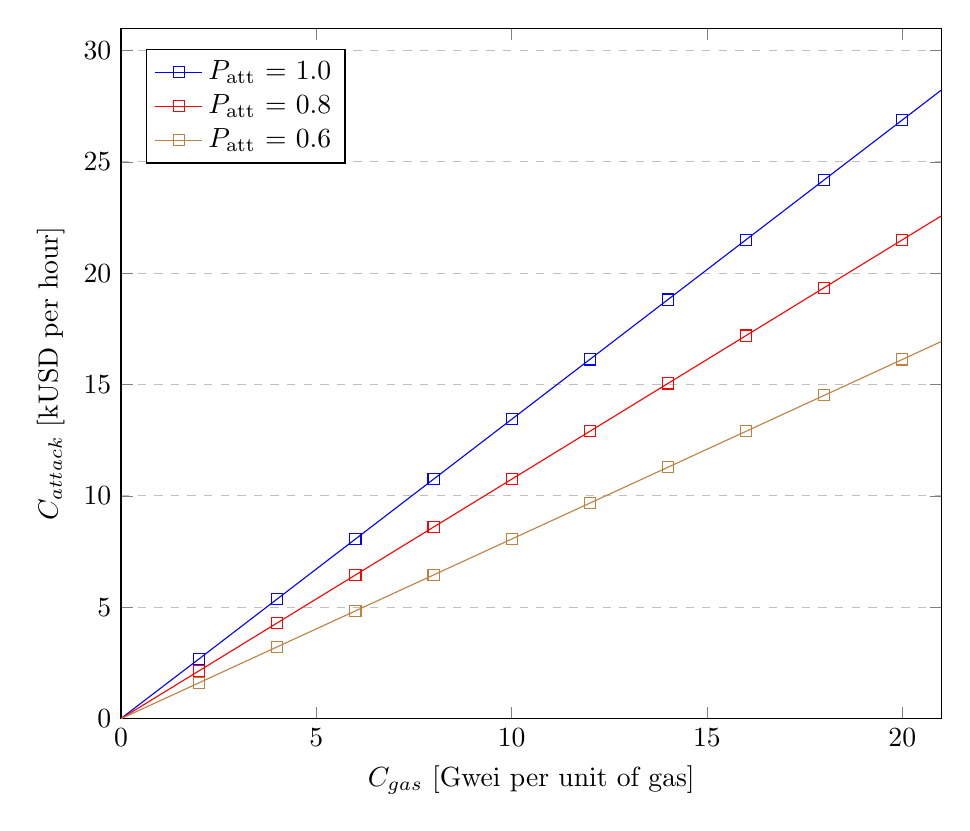
\begin{tikzpicture}
\begin{axis}[
    xlabel={$C_{gas}$ [Gwei per unit of gas]},
    ylabel={$C_{attack}$ [kUSD per hour]},
    xmin=0, xmax=21,
    ymin=0, ymax=31,
    xtick={0,5, 10, 15, 20},
    ytick={0, 5, 10, 15, 20, 25, 30},
    legend pos=north west,
    ymajorgrids=true,
    grid style=dashed,
]
 
\addplot[
    color=blue,
    mark=square,
    ]
    coordinates {
    (-2,-2.668)(2,2.688)(4,5.376)(6,8.064)(8,10.752)(10,13.440)(12,16.128)(14,18.816)(16,21.504)(18,24.192)(20,26.880)(22,29.568)
    };
    
\addplot[
    color=red,
    mark=square,
    ]
    coordinates {
    (-2,-2.150)(2,2.150)(4,4.300)(6,6.450)(8,8.600)(10,10.750)(12,12.900)(14,15.050)(16,17.200)(18,19.350)(20,21.500)(22,23.650)
    };
    
\addplot[
    color=brown,
    mark=square,
    ]
    coordinates {
    (-2,-1.612)(2,1.612)(4,3.226)(6,4.838)(8,6.451)(10,8.064)(12,9.676)(14,11.289)(16,12.902)(18,14.515)(20,16.128)(22,17.741)
    };
    \legend{$P_{\mathrm{att}}$ = 1.0, $P_{\mathrm{att}}$ = 0.8, $P_{\mathrm{att}}$ = 0.6}
 
\end{axis}
\end{tikzpicture}
\caption{Hourly cost of a theoretical DDoS attack in thousands of USD.}
\label{fig:ethddos}
\end{figure}

As can be seen in Figure \ref{fig:ethddos}, even when the attacker pays only 2 Gwei for single unit of gas and desires to establish a 60\% reduction of throughput (which would not harm the Ethereum network significantly at current state) by generating hostile transactions, it would come at a cost of approximately 2.30 ETH, or 1612 USD$^\star$ per hour. Gas price of 2 Gwei is considered to be a standard price at the time of writing. It is used in transactions for confirmations times of around few minutes, when network is moderately congested. As mentioned before, attackers would need to use a much higher gas price to block the significant part of network's throughput. A more realistic figure to look at would be gas price of around 10-15 Gwei and $P_{\mathrm{att}}$ of 0.8. An hour of such an attack would cost tens of thousands of dollars to perform. Even if the attack is performed using transactions with high gas price $N$, regular users would still be able to generate transactions and get them added to new blocks by simply using gas price of $\geq N$, which is larger then the DDoS transactions' gas price.

One more thing to consider, regarding DDoS attacks on Ethereum, is that the gas block limit is gradually increasing, as the total network hashpower grows. Recent increase from approximately $6.7 \cdot 10^6$ to around $8 \cdot 10^6$ gas happened in December 2018. Further growth of block gas limit would make theoretical DDoS attacks even more expensive, as it would lead to increased throughput of the network.

\paragraph{51\% attacks}
One of the most common potential threats to public blockchain-based systems are the \textit{\glspl{51 attack}}. The consensus principal in most blockchain based systems is indeed very much the same, as how the presidential elections in democratic countries are held, namely that the candidates need to gain the majority of votes, in order to be elected. The same principal is applied in nearly all public blockchains. In order for a new block to be added, it has to be accepted by the majority of nodes. Thus, 51\% attack refers to an attack on a blockchain by a group of miners controlling more than 50\% of the network's mining hashrate, or computing power. The possession of a total hashrate percentage of over 50\% would result in potential attackers being able to prevent new transactions from gaining confirmations, allowing them to halt payments between some or all users. They would also be able to reverse transactions that were completed while they were in control of the network, meaning they could double-spend digital assets. However, if such an attack was to take place, the attackers would still be unable to change the contents of previous blocks or generate new coins and tokens in cryptocurrency-related blockchains.

In case of Ethereum, such an attack would be possible, but highly unlikely to happen. Mining in general is such a popular activity nowadays, making Ethereum's hashrate relatively high, as shown in Figure \ref{fig:ethereumhashrate}. Therefore, the possession of more that 50\% of Ethereum's hashrate by a single person or organization is very unlikely, as it requires enormous resources. However, this enormous popularity and huge hashrate of Ethereum has resulted in solo mining being no longer viable, as the time to confirm a block by mining solo is often measured in months, or even years in case of some popular networks, depending on the size of mining operation and luck factor. This led to the introduction of, so called, \textit{\gls{pool mining}}. Its concept is that the miners join a pool, which distributes nonces to different mining subnodes (in other words, miners are cooperating between eachother to find blocks, when pool mining). Miners then get a share of total block reward from the blocks that have been found by the pool. This basically means that the mining pool is being in the possession of all the contributed hash power. This can lead to security concerns if the pool's total hashrate becomes more than a half of the total network hashrate, as it enables the pool to execute such 51\% attack.

\begin{figure}[H]
\centering
\includegraphics[scale=0.49]{images/ethereumhashrate.png}
\caption{Overall Ethereum network hashrate \textnormal{\citep{ethhashrate}}.}
\label{fig:ethereumhashrate}
\end{figure}

However, hitting 51\% network control is not a guarantee of success, it is just the point where success is likely. In fact, a node could attempt this sort of attack with much less network control, but the odds of success would be very low \citep{51perattack}. 

There is an obvious conclusion that can be drawn, regarding the 51\% attacks. Network's exposure to such attacks proportionally decreases, when the overall network hashrate increases. Smaller blockchain networks are obviously more exposed to 51\% attacks, than larger, more popular networks, that possess higher hashrates.

\paragraph{Man-in-the-middle attacks}
A \textit{\gls{man-in-the-middle attack}} is a type of cyberattack, in which a malicious actor inserts him/herself into a conversation between two parties, impersonates both parties and gains access to information that the two parties were trying to send to each other. In case of such attack, a malicious actor may try to intercept, send and receive data meant for someone else, or not meant to be sent at all, without either outside party knowing until it is too late \citep{mitm}.

Any system, that communicates via the Internet is exposed to such attacks. Thus, the communication channel between the user and the service, whether it is a blockchain or a server, has to be secure. A common technique, which is used in order to achieve that is digital signatures. Digital signatures ensure that the contents of the message, which was transmitted through the channel, were not tampered with, or changed.

\paragraph{Smart contracts and security flaws}
Ethereum is an extremely secure network. As was discussed before, it has a sufficient enough protection against 51\% attacks and DDoS attacks are extremely costly and impractical to perform. However, it is still possible to implement buggy smart contracts, that would introduce potential security flaws. The DAO hack, which was briefly mentioned in \ref{section:transparency}, happened due to that particular reason, as there was a bug in the DAO smart contract, which was discovered by the attacker and exploited. Thus, the developers need to be extremely careful, during the implementation process, in order to prevent such events from happening. A tool, which might be useful for that purpose is called Oyente. This tool can be used to test the smart contract code for bugs and security breaches \citep{oyente}.

\paragraph{Encryption in centralized systems}
There are many cryptographic solutions that can be chosen for the implementation of centralized systems. There are countless different algorithms out there, that are typically using two main cryptographic approaches: symmetric and asymmetric.

\textit{\Gls{symmetric encryption}} is the simplest kind of encryption that involves only one secret key to cipher and decipher information. Symmetrical encryption is an old and best-known technique. It uses a secret key that can either be a number, a word or a string of random letters. It is a blended with the plaintext of a message to change the content in a particular way. The sender and the recipient should know the secret key that is used to encrypt and decrypt all the messages. Blowfish, AES, RC4, DES, RC5, and RC6 are examples of symmetric encryption. The most widely used symmetric algorithm is AES-128, AES-192, and AES-256. The old and outdated DES algorithm is now used in a 3DES configuration, which basically involves execution of DES three times. The main disadvantage of the symmetric key encryption is that all parties involved have to exchange the key used to encrypt the data before they can decrypt it.

\textit{\Gls{asymmetric encryption}} is also known as public key cryptography, which is a relatively new method, compared to symmetric encryption. Asymmetric encryption uses two keys to encrypt a plaintext. It is important to note that anyone with a secret key can decrypt the message and this is why asymmetrical encryption uses two related keys to boosting security. A public key is made freely available to anyone, while private key is kept a secret. A message that is encrypted using a public key can only be decrypted using a private key, while also, a message encrypted using a private key can be decrypted using a public key. Security of the public key is not required because it is publicly available and can be passed over the Internet. Asymmetric key has a far better power in ensuring the security of information transmitted during communication. Asymmetric encryption is mostly used in day-to-day communication channels, especially over the Internet. Popular asymmetric key encryption algorithm includes RSA, DSA, Elliptic Curve (used in Ethereum and many other blockchains), PCKS and others \citep{pubvssym}.

\begin{figure}[H]
\centering
\includegraphics[scale=0.55]{images/pubpriv.png}
\caption{Public key cryptography (A) and symmetric encryption (B) illustrations.}
\label{fig:keygenerationether}
\end{figure}

Different encryption algorithms are good in different aspects and bad in other ones. For example, symmetric encryption algorithms are significantly faster than the asymmetric ones, however, they involve transmission of private keys before the communication can take place, thus introducing a risk of private key being intercepted. It is important to use encryption algorithms that are right for the task at hand.

\paragraph{Possible encryption mechanism in smart contracts}
Theoretically, the smart contracts can easily store 256-bit application-specific public keys of addresses, using data structure, called \texttt{mapping}. It maps key value pairs, where the keys could potentially correspond to users' Ethereum addresses and the values could correspond to the application-specific public keys. As mentioned in \ref{section:transparency}, Ethereum is completely transparent, thus the sensitive private information of users in the blockchain based Secure Package system would be exposed to the public, if not encrypted. 

The solution for that could be to generate individual Secure Package key pairs off-chain, store private keys securely at the user's computer and upload public keys to corresponding mappings inside of the smart contract. The reason behind generation of keys off the chain is that it prevents serious security and efficiency issues with on-chain generation.

Thus, it is theoretically possible to create encryption protocols for data transfer and storage in Ethereum. The keys would need to be 256-bit long, while still being able to provide secure encryption that can withstand hostile intrusion attacks. This can be achieved with elliptic curve cryptography in rather the same manner, as how Ethereum addresses' key pairs are generated. This is covered in greater detail in the next paragraph.

\paragraph{Key distribution and generation in Ethereum}
Public key cryptography is widely used in blockchain-based systems. Private keys are used to sign the transactions and generate public keys. As mentioned before, the Ethereum blockchain is completely transparent. This makes generation and distribution of private keys on-chain a very bad idea, as the keys can be intercepted by anyone, thus making them useless.

To solve these issues, the private key generation process for new Ethereum accounts is performed off-chain by taking any random 256-bit number and storing it safely off-chain. This 256-bit number acts as a private key. Public key is then generated from that random private key, which in its turn generates the account address. Key pairs are used for verification purposes and the address is used for indexing.

\begin{figure}[H]
\centering
\includegraphics[scale=0.62]{images/ethaddr.png}
\caption{Generation of keys and addresses in Ethereum. Private key is stored off-chain. Generation process involves the ECDSA algorithm, along with Keccak256 hashing algorithm \textnormal{\citep{ethyellow}}.}
\label{fig:keygenerationether}
\end{figure}

Using this approach, the private key is never being sent over the blockchain. This makes it very difficult for the intruder to access the account, assuming that a properly chosen seed has been used to randomly generate the private key. The are theoretically only two ways to break such 256-bit ECDSA private key. The first and most straightforward way would be to try all of the possible key combinations, which might take billions of years with the current technology, as there are $2^{256}$ possible keys. This approach is often referred to as "brute force". The second way is to solve the Elliptic Curve Discrete Logarithm Problem (ECDLP), which the ECDSA algorithm is based on. Rough estimates of solving this problem by using raw processor power is around $38.5 \cdot 10^{20}$ years, assuming that the encryption has been done properly and that private key possesses high degree of randomness. There are other approaches to solving this problem, by exploiting mathematical properties, such as hyperelliptic curves and elliptic curves with small complex multiplication fields \citep{ecdsa}.

Ethereum's public key cryptography, which is based on ECDSA, is considered being very secure, despite using rather short key size, compared to RSA, in which key lengths of up to 4096 bits are used \citep{rsakeys}. This has to do with the complexity of underlying mathematical problem. The mathematical problem that RSA is based on is prime number factorization, which is a lot less complex than ECDLP. That is the reason for a rather short key size in ECDSA.

Nevertheless, as long as the private key file is securely stored on the user's computer, there is little to no risk of the account being broken by an intruder.

\subsubsection{Scalability, performance and constraints} \label{section:scalability}

\paragraph{Availability and downtime}
Some client-server systems are very vulnerable to server breakdowns, as they, in many cases, drastically reduce service's bandwidth, or make the service stop working altogether. High availability and low downtime is a must for a highly congested client-server architecture. These factors are strongly dependent on the server infrastructure, its degree of decentralization, integration of data migration tools and possesion of back-up servers. Ethereum, however, possesses high degree of availability, due to its decentralized nature. If one of the nodes fail, there are still plenty of other nodes available.

\paragraph{Unpredicted confirmation delay}
When dealing with blockchain based systems, it is important to consider that a newly generated transaction has to be added to a block, before being confirmed and validated. This process may take different amounts of time, depending on the network's current state and network's target block time. Ethereum's target block time of 15 seconds is quite short, comparing to other blockchains like ZCash and Bitcoin, whose block times are 2.5 and 10 minutes respectively. However, even if a transaction is included into the blockchain's next block by the miners, the data will not become a part of the blockchain until the block has been mined. Target block time does not provide any guarantee that the block will be added to the chain within the target time, as the mining process itself involves a degree of randomness. Thus, the block finding time is heavily dependent on luck factor and is impossible to predict. A test, in which actual block times of 10000 blocks of Ethereum are analyzed can be found in Figure \ref{fig:ethtimetest} of Appendix \ref{section:blocktimes}.

There is as well no guarantee on the number of new blocks being found before the generated transaction itself will be included into a new block. This is heavily dependent on the gas price, which is chosen for the transaction. In applications that need to perform a large number of smart contract function calls, there is a trade-off to be made between the cost and latency, as faster response times will be a lot more expensive to achieve (detailed discussion about that is provided in \ref{section:economics}).

Introduction of such delay makes the implementation of applications, in which the responsiveness is a key factor, impossible. Such example is applications for real time monitoring. In some systems it is crucial to be notified about a problem, or a system state change as soon as possible. By using Ethereum to power such application, operators in the control room would not be notified about, for example, a potential problem which generates an alarm, before the transaction, that was generated by the alarm contract, was mined (which, as explained before can be take indefinite amount time). In such systems it is much more viable to use client-server architecture-based alarm system.

\paragraph{Ethereum's throughput and scalability} 
One of the main things to consider, when talking about a system's performance, is its maximum throughput and how it can be increased when needed. In Ethereum, the maximum throughput of the network is defined by the gas limit of the blocks and their frequency, using the following formula:

\begin{equation} \label{eq:eththroughput}
T_{\mathrm{net}} = \frac{1}{t_b} \cdot L_b = \frac{L_b}{t_b}
\end{equation}

Ethereum's block time $t_b$ is equal to 15 seconds, which can be converted to 1/240 hours. Block gas limit is equal to $8 \cdot 10^6$ at the time of writing. This block gas limit $L_b$ can be changed by miners, depending on overall network hashrate and congestion. Thus, by inserting the values into Equation (\ref{eq:eththroughput}), the current total throughput rate of Ethereum, $T_{\mathrm{net}}$, is approximately $1.6 \cdot 10^9$ gas/hour.

A basic Ethereum transaction for token transfer consumes 21000 gas, thus the current theoretical transaction capacity of Ethereum is approximately 76200 tx/h, assuming that none of the contracts executes any code. The theoretical transaction capacity is significantly reduced, when introducing transactions that require computational effort. 

The block gas limit has historically been increasing as a result of the growing hashrate of Ethereum network. The main reason for the existence of gas limit is to enable consensus participation of smaller mining nodes, thus further decentralizing the network. All of the transactions and their associated code has to be verified by the nodes. So without a proper limit on amount of gas per block, the nodes could potentially be overwhelmed. 

As mentioned earlier, increased congestion of the network can be addressed by adjusting the block gas limit $L_b$. The result of that gas limit would lead to a proportional increase in throughput in terms of gas, according to Equation (\ref{eq:eththroughput}).

\begin{figure}[H]
\centering
\includegraphics[scale=0.49]{images/gasblocklimit.png}
\caption{Gas block limit increase. Limit has been increased by four times since October 2016 to accommodate the growing congestion \textnormal{\citep{ethgaslimit}}.}
\label{fig:ethergasblocklimit}
\end{figure}

Nevertheless, despite the throughput's flexibility, which is provided by the gas block limit adjustment, it would be wrong to say that Ethereum possesses good scalability, as its theoretical average throughput of around 21 transactions per second is extremely poor, in comparison to typical client-server systems. The throughput needs to be scaled by an extremely large factor, in order for Ethereum network to possess comparable throughput to a typical client-server system, which can not be achieved fast enough by just increasing the gas block limit alone. 

\paragraph{Storage and memory}
Each and every smart contract has its own independent storage. That storage is virtual and is structured in terms of indexable key-value pairs. There are $2^{256}$ key-value pairs in each contract, with each pair having a capacity of storing 32 byte words, that results in a storage capacity of $2^{261}$ bytes. Thus, there is no doubt that there is plenty of storage, which is an understatement (as it turns out, a single smart contract has a theoretical capacity to store all of the humanity's data billions and billions times over).

This all sounds really good on paper, however, there is a cost that comes with using this storage. Storing a single 256-bit word consumes 20000 gas ({\small SSTORE} operation when the value is altered from zero to non-zero), excluding the base transaction cost of 21000 gas. In order to upload large files to smart contracts, they would need to be broken down to small 256-bit chunks and stored in different key-value pairs, using {\small SSTORE}. Equation (\ref{eq:filestorage}) derives the cost of storing a file in a smart contract.

\begin{align} \label{eq:filestorage}
C_{\mathrm{store}} = C_{\mathrm{gas}}\left(\frac{Q \cdot G_{sstore}}{256} + G_{tx}\right) \cdot 10^{-9} \cdot C_{ETH}  
\end{align}

Here, $Q$ is the file size. The file size is given in megabytes (1 megabyte is equal to $8 \cdot 10^6$ bits). Gas consumption of a single {\small SSTORE} operation, $G_{\mathrm{sstore}}$, is 20000. Base transaction cost, $G_{\mathrm{tx}}$, is 21000. Assuming that a gas price, $C_{\mathrm{gas}}$, of 2 Gwei was used, the following equation is derived.

\begin{align}
C_{\mathrm{store}} &= 2 \cdot \left(\frac{8 \cdot 10^6 \cdot 20000 \cdot Q}{256} + 21000\right) \cdot 10^{-9} \cdot C_{ETH} \approx 1.25 \cdot C_{ETH} \cdot Q
\end{align}

Thus, a single megabyte of storage costs approximately 1.25 ETH, or 875 USD! That is an exceptionally high price to pay, considering that services like Dropbox offer cloud storage of 2 terabytes at a monthly cost of around 12 USD \citep{dropbox}.

Another limitation on storage of large files in smart contracts is the gas block limit $L_b$. A transaction may obviously not exceed the gas block limit, as it would be impossible for it to be included in a block otherwise. Considering the current block gas limit of $8 \cdot 10^6$, the theoretical maximum amount of {\small SSTORE} operations triggered within a single transaction is derived using following equation.

\begin{align}
N_{sstore} = \floor[\Bigg]{\frac{\left(L_b - G_{tx} \right)}{G_{sstore}}} = \floor[\Bigg]{\frac{\left(8 \cdot 10^6 - 21000\right)}{20000}} = 389
\end{align}

Thus, there will be an overhead of 21000 gas approximately each 389 {\small SSTORE} operations (which corresponds to storage of 99584 bits). Equation (\ref{eq:filestorage}) needs to be modified with that overhead in mind.

\begin{align} \label{eq:newstorecost}
C_{\mathrm{store}} = C_{\mathrm{gas}}\left(\frac{Q \cdot G_{sstore}}{256} + G_{tx}\left(\frac{Q}{256}\middle/\floor[\Bigg]{\frac{\left(L_b - G_{tx} \right)}{G_{sstore}}}\right)\right) \cdot 10^{-9} \cdot C_{ETH} 
\end{align}

By numerically solving (\ref{eq:newstorecost}), the cost of storage turns out to be equal to approximately 1.266 ETH, or 886.20 USD$^\star$ per megabyte.

Additional consequence of splitting the file storage process into multiple transactions, spanning multiple blocks, is that the upload might take a long time, as the target block time is around 15 seconds. Assuming that each and every following block is filled with file content upload transactions until the storage process is completed, the average transmission speed would be 99.6 kilobits every 15 seconds, which translates into roughly 6.6 kilobits second. Even the dial up modems from the 90s had faster speeds of around 56 kilobits per second \citep{dialup}. At that rate the storage process of one megabyte would span over 81 blocks, thus taking approximately 20.25 minutes to complete, assuming that no other transactions are being included in any of those 81 blocks (but the last one), which is very unlikely.

However, once the data is added to the smart contract's storage it is free to access, using \texttt{get()} methods.

\paragraph{Scalability and performance of centralized systems}
Systems that are using a client-server architecture are relying heavily on the servers, when dealing with increased amount of traffic. There are countless server solutions, which sparks a competition among server providers. This competition drives the technology forward, thus making single server units being able to handle more and more traffic.

Servers are typically located in server racks inside of big data centers. The process of adding additional server units to accommodate the increased amount of traffic is typically as easy as stacking more units on top of eachother on a server rack. Increased storage demands can be addressed by upgrading existing storage disks to larger capacities, or just adding more of them. However, this can sometimes require some maintenance downtime.

\paragraph{Choice of key sizes}
As mentioned before in this section, extensive computation complexity and large requirements on storage of the smart contracts leads to extremely high gas consumptions. That is why it is very important to go as far as optimizing each and every variable in the smart contract code as it would significantly reduce gas consumption of execution and contract deployment. For optimization purposes, ECDSA 256-bit keys are used in Ethereum, as well as many other blockchains. The reason for that is the rather short key size, which is beneficial in terms of gas and computational effort savings.

One of the most common asymmetric cryptographic algorithms, RSA, which is used in many centralized applications, typically uses 1024- and 2048-bit keys for encryption, which is considerably larger then then 256-bit keys in ECDSA cryptography in Ethereum. The reason for that is that ECDSA is more cryptographically complex than RSA, as was described in \ref{section:analysisencryption}, which leads to smaller key sizes needed.

\paragraph{Symmetric key cryptography and public blockchains}
As mentioned in \ref{section:analysisencryption}, transmission of private keys on the blockchain is a really bad idea due to its transparency. Thus, symmetric encryption algorithms, such as AES and DES, can not be implemented on Ethereum, as the secret key would be visible to everyone on the network, making it rather useless. This is obviously not the case in the centralized systems as long as a secure communication channel is established.

\paragraph{Implementation constraints}
Blockchain is a relatively new technology. At the time of writing, there are only a few blockchains that support smart contract scripting functionality. Smart contracts are written in contract-oriented programming languages, out of which Solidity is the superior one. Solidity is considered being quite low-level to make it easier to optimize code, as storage and instruction executions are quite expensive in Ethereum. Solidity is also highly criticized for some of it's design flaws, such as static 256-bit word lengths, confusing type names (for example, \texttt{bytes32} is a byte array that has a size of 256 bits and \texttt{uint32} is an integer that has a size of 32 bits, which can be very confusing), no string manipulation support, no null pointer support, no floating point numbers and so on \citep{soliditybad}. 

When developing non-blockchain applications, there is a great choice of different design patterns that can be used for development, as well as a wide selection of available programming languages for all needs. This gives programmers a lot more freedom during the implementation and system design phase. The freedom of implementation approaches is strongly dependent on the type of application being implemented. The point is that the range of possible applications that can be built on a client-server architecture is significantly larger than the range of applications that can be built on Ethereum.



\subsubsection{Reusability and modifiability} \label{section:reuse}
Blockchain applications are typically easy to deploy, reuse and modify, as long as the contract-oriented language Solidity allows it. Deployment of additional services on smart contracts is a relatively easy process. Usage of an API is desired in the centralized systems, as it increases the quality reusability and modifiability quality attributes.

\paragraph{Connecting multiple platforms to DApps}
Once a DApp is deployed onto the chain, it, if implemented properly, can be used as a core foundation for a platform with similar purpose. Multiple platforms can be connected to the same DApp in the same way as multiple DApps are connected to the Ethereum network. Individual smart contracts do not have any defined maximum throughput, thus, increased transaction density, that targets a specific smart contract, does not degrade its performance (more specific details on that topic can be found in \ref{section:scalability}). There is as well no need for any additional hardware components in case of increased traffic, as it is with centralized systems.

\paragraph{Modifying and reusing centralized applications}
Centralized applications' reusability and modifiability is highly dependent on the quality of implementation. Usage of design patterns that improve the code's reusability and modifiability is highly beneficial, in case of those quality attributes being important for a particular system. Typical design patterns, that are used for that purpose, are the Adapter and Facade design patterns.

In client-server applications, a good way to improve a system's reusability, modifiability and scalability is to implement an application programming interface (API), that handles the communication between the client side (frontend) and the server side (backend). In other words, API's task is to connect various components of the application. Usage of an API for component communication follows the guidelines for Facade design pattern. An example of that is illustrated in Figure \ref{fig:apipattern}.

\begin{figure}[H]
\centering
\includegraphics[scale=0.59]{images/facadeapi.png}
\caption{Illustration of API Facade design pattern.}
\label{fig:apipattern}
\end{figure}

Usage of an API as a hub for communication, results in individual components of the system being independent of eachother. Thus, different parts of the system can easily be modified or replaced, when needed, without affecting other parts of the system. 

APIs are, in some cases, used to introduce the functionality of integrating applications to other services. For example, Google Maps application has an API, which can be integrated into other web applications.

\paragraph{Modifying smart contracts and DApps}
As Ethereum is completely transparent, all source code of deployed smart contracts is available to the public. This follows the same ideology as most of the open-source software, namely that users have a freedom of extending and modifying the code in a way that they would like to. 

Many DApps, including the decentralized version of Secure Package adopt a token payment system by the customized ERC20 tokens. As all of the ERC20 tokens have to follow a specific standard, that is defined by the interface contract in Figure \ref{fig:erc20interface}, it is very easy to modify the existing payment system by deploying a contract, that follows that interface.

\begin{figure}[H]
\centering
\includegraphics[scale=0.69]{images/erc20.png}
\caption{ERC20 interface contract \textnormal{\citep{erc20}}.}
\label{fig:erc20interface}
\end{figure}
\subsubsection{Economic aspect} \label{section:economics}
Economic aspect is very important to take into consideration, as it is essential, when designing centralized applications, especially, when there is a central authority involved. Blockchain-based systems often rely digital assets in form of cryptocurrencies, which are extremely volatile. An introduction of sensor support opens up opportunity for logistics companies to make profit from adding sensors to packages.

\paragraph{Price volatility of cryptocurrencies}
The nature of Secure Package service is, whether it is Ethereum network or a centralized server architecture that is used for data handling, the logistics process stays the same, apart from usage of sensors for monitoring. The time it takes for the item to reach the buyer is measured in days, which poses a problem when using a cryptocurrency-based payment system. The reason for that is that cryptocurrencies tend to be extremely volatile from economic standpoint.

In order to demonstrate application of that in real world, consider a case, in which buyer $A$ agreed to purchase an item from seller $B$ using the Secure Package service, that was built using blockchain architecture, for the price of 1 ETH back in 27th of May 2017. Assuming that $B$ sent the item on the following day and that shipment process took two days, the package was received and its condition was confirmed by $A$ on 30th of May. Thus, it took the total of three days for the seller to receive the payment from the point of agreement. Currently, vast majority of people are measuring the value of items in fiat money. When trading goods in Ether, people would naturally think of fiat value and then convert it to Ether. On the 27th of May 2017, the price of ETH had its low of around 130 USD. On the afternoon of 30th of May, the price jumped all the way up to 215 USD, which is an increase of around 65\% over the course of only three days \citep{ethprice}. Thus, the buyer had to pay 65\% more for the item in fiat currency equivalent.

Usage of fiat money for payments is a lot less volatile, however it is not possible to integrate such fiat payment system into a blockchain. The closest possible solution for that is usage of, so called, "stable coins", which are covered in the next paragraph.

\paragraph{Stable coins and associated issues}
There are currencies, such as Tether \citep{tether}, which are often referred to as "stable coins". The ideology behind those currencies is that they are pegged to the value of a given fiat currency one-to-one. In Tether, this one-to-one exchange rate is achieved by maintaining a US dollar reserve. Each issued Tether is corresponding to one US Dollar in the reserve, maintained by a company, called Tether Limited. This results in Tether being worth approximately one US dollar per token. An integration of such "stable coin" functionality could potentially solve the issue of volatility, by creating an ERC20 token with a money reserve. However, this requires a third party, which maintains the reserve fund, thus making the whole token system centralized. The third party presence and its potential disadvantages were discussed in \ref{section:analysisthirdparty}.

\paragraph{Introduction of sensor support}
Many companies are using marketing strategies, in which they charge customers more money for additional features in a product. An introduction of sensor support for logistics process may not only provide additional security for the packages, but can also benefit the logistics company economically. Implementation of sensors, such as accelerometers, temperature and humidity indicators, into the logistics process would open up a possibility of generating more revenue from package delivery, by charging extra money for inclusion of sensors.

\paragraph{Gas usage and transaction density}
Each and every interaction that is processed by Ethereum network requires a transaction fee. This fee is measured in specific units, called gas in Ethereum and it is heavily dependent on current congestion of the network (high congestion results in higher gas price required to process a transaction within a given time frame). At the time of writing, the average plain transaction that does not execute any specific smart contract code consumes 21000 gas units, which costs around 0.00004 ETH (which is around 0.03 USD$^\star$) to process, given the current standard gas price of 2 Gwei \citep{ethgasstation}. However, computations, that are executed by the smart contracts consume a fixed amount of gas per computation. Thus, method calls, that require large amounts of computations, consume more gas. This leads to a conclusion, that a lot of time and effort needs to be dedicated to reduce function calls and optimize executable calls in smart contracts in order to avoid large transaction fees.

Introduction of sensor support, especially GPS tracking, introduces a potential problem of bottlenecking communication bandwidth of sensor data. The reason for that does not lie in the technical aspect of the system. As mentioned before, every interaction with smart contracts consumes gas. All of the information about the agreement, including GPS sensor data, is stored inside the smart contract. Thus, to update the GPS data, an interaction with the smart contract, that updates the latitude and longitude values, is required. Execution of variable update operation $G_{sreset}$ has a base gas consumption of 5000. Thus, the amount of gas, which is consumed by updating two variables inside the smart contract, is equal to at least 10000. Apart from execution of code, the transaction itself has a base gas consumption of 21000, whether it is a simple transfer of tokens from one address to another, or an execution of some advanced algorithm on a smart contract, that requires a lot of computational resources. Thus, continuous communication with sensors during the logistics process would lead to a large number of generated transactions, that consume at least 31000 gas. This is not really a problem, when dealing with sensors like accelerometers, where the only relevant data is whether the threshold value was violated. This data can be sent to the contract once the logistics process is finished, thus only generating one transaction. GPS tracker, however, becomes quite useless, unless it communicates with the application somewhat often.

In order to get an understanding of the scope of this issue, the following scenario is considered. Assuming that the logistics process takes exactly two days to complete and that the included GPS sensor communicates with the contract once a minute, simple math reveals that 2880 transactions are generated during that timeframe. Each transaction consumes 31000 gas (21000 for performing the transaction and around 10000 for performing the update of each variable, depending on the size of the variables), which results in $8.928 \cdot 10^7$ units of gas consumed in the process. Now, when dealing with system design, it is important to consider the worst possible cases. As mentioned before, the gas price needs to be increased, when network becomes more congested, otherwise, the transaction will not be mined until the congestion decreases, which can take days. Historical data shows that the average gas price was approximately 9 Gwei on the 10th of January 2018. That big of a gas price was resulted from a large amount of transactions being processed around that day. Considering the gas price of 9 Gwei, each sensor communication would come at a cost of 0.00028 ETH. This sums up to approximately 0.81 ETH during two day transfer, which is around 567 USD$^\star$. It is an understatement to say that this is a large amount of money to spend for this kind of functionality, unless the contents of the package are of high value. In order to avoid that problem, the frequency of sensor communication needs to be significantly reduced, which indirectly introduces a bottleneck.

\paragraph{Gas usage and storage}
Apart from economic gas related issues, regarding increased transaction density, there are also issues associated with storage on Ethereum blockchain. As mentioned in Section \ref{section:scalability}, each smart contract has $2^{261}$ bits of individual virtual storage, which is a huge amount. However, as was discovered in Section \ref{section:scalability}, this storage is extremely expensive. Each {\small SSTORE} operation, that stores a 256-bit word into the smart contract's empty space consumes 20000 gas.

When selling items online, a good picture and detailed description increases the item's selling potential dramatically \citep{ebay}, thus it is essential and very important to support inclusions of pictures and descriptions in the adverts, when creating a merchandise trading platform. Table \ref{tab:imgdescscenarios} illustrates different gas consumption scenarios, in which image and description upload is performed. The average image size is assumed being 100 kilobytes (after compression, which is assumed being done off-chain before the upload). 

Table \ref{tab:imgdescscenarios} shows that it costs a total of 183.90 USD$^\star$ to post an advert, that consists out of two heavily compressed images and a short description. By analyzing the table, it is easy to spot that additional images are extremely expensive to upload. An important note is that 100 kilobytes per image is a very generous approximation, as it is not uncommon for a typical 1024x768 JPEG image to have a size of around 1 megabyte, which is 10 times larger, than was considered in the scenarios. Greater image sizes and longer descriptions would be proportionally more expensive to upload, as derived in Equation (\ref{eq:newstorecost}). It is quite obvious, that storage of large files in Ethereum is not viable due to the high cost.

\begin{table}[H]
\centering
\begin{tabular}{| c | c | c | c |}
\hline
\textbf{Advertisement scenario}& \textbf{Gas used} & \textbf{ETH} & \textbf{USD$^\star$}\\
\hline 
0 images, 100 characters description & $1.3 \cdot 10^5$ & 0.0002592 & 0.18\\
0 images, 200 characters description & $2.0 \cdot 10^5$ & 0.0003993 & 0.28\\
0 images, 400 characters description & $3.3 \cdot 10^5$ & 0.0006614 & 0.46\\
1 image, 200 characters description & $6.6 \cdot 10^7$ & 0.1316073 & 92.13\\
2 images, 100 characters description & $1.3 \cdot 10^8$ & 0.2627172 & 183.90\\
\hline
\end{tabular}
\caption{Different uploading scenarios. Gas price of 2 Gwei was considered. Values within the table were derived, using Equation \textnormal{(\ref{eq:newstorecost})}.}
\label{tab:imgdescscenarios}
\end{table}

\paragraph{Removal of third party}
Introduction of a blockchain architecture has a potential to remove the third party aspect, in form of Blocket, from the equation. It is obvious that companies, that are maintaining a service, need to get some sort of payment in return. In case of Blocket Secure Package, dedicated servers, support staff and maintenance technicians are needed to keep the service operational. Blocket is a profit seeking organization, thus it is not hard to guess that the service would become cheaper if the third party involvement was removed. And so is the case, as it costs around 3 USD less to send a small package directly though DBSchenker, then by using Blocket Secure Package. However, what a user does not get, by just sending the package directly through DBSchenker, is the cash-on-delivery service and an opportunity of contacting Blocket's customer service if something goes wrong with the transfer.
  





\subsubsection{Environmental aspect} \label{analysis:environmental}

There are differences between the architecture models, regarding the environmental aspect. Usage of current version of Ethereum poses enormous environmental issues, as execution of proof-of-work algorithm is very power consuming. Servers and their cooling solutions are getting more efficient and sophisticated nowadays, thus making the model of using a centralized server more power efficient and environmentally friendly.

\paragraph{Mining and power consumption}
Execution of proof-of-work algorithms (ofter referred to as mining) is a very power hungry process. At the time of writing, the total hashrate of Ethereum network is fluctuating around 260 TH/s and is steadily increasing \citep{ethhashrate}. The most efficient hardware for mining most ASIC-resistant cryptocurrencies are graphic cards with chips from manufacturers NVidia and AMD. In order to get an idea of Ethereum network's total power consumption, let's assume that all of the miners are using the most common and widely used graphics card for this purpose, AMD RX580, which has a hashrate of around 30.2 MH/s and consumes around 135 Watts in the process \citep{whattomine}. Simple math shows, that the total hashrate of Ethereum corresponds to hashpower of around 8.6 million RX580s, which draw a whopping 1.16 TW of power combined! According to The World Bank, this figure corresponds to power consumption of the entire country of Lithuania \citep{worldpowerconsumption}. Clearly, from environmental standpoint, this is a big issue. The situation is getting worse, as mining becomes more and more popular, due to the activity of running mining hardware being profitable from economic standpoint. An illustration of that increased popularity can be seen by studying recent development of Ethereum's hashrate. By looking at the graph in Figure \ref{fig:ethereumhashrate} of Section \ref{section:analysisencryption}, we can see, that the total hashrate of Ethereum network was doubled between December 2017 and March 2018, which is a period of 4 months.

Security of public blockchain networks, such as Ethereum, is strongly dependent on the total hashpower, due to increased protection against 51\% attacks, as described in \ref{section:analysisencryption}. It is possible to run an instance of Ethereum network with only a small fraction of today's hashrate, however, this would make the blockchain fragile against 51\% attacks.

The bottom line is that in order to run any secure blockchain network that uses proof-of-work consensus mechanism, it has to have a significant number of miners. Each piece of hardware, that is used for verification purposes consumes power. Having a large number of mining hardware constantly running is bad for the environment and the situating is getting worse, with the hashrate increasing every day that comes.

\paragraph{Proof-of-stake}
Not all blockchain networks are using proof-of-work as consensus mechanism. Another mechanism, which currently is gaining popularity and recognition, is called \emph{\gls{proof-of-stake}}. Its principal is that the nodes are locking a number of assets (in case of cryptocurrencies it is tokens, or coins) into validator nodes to secure the network. In proof-of-stake based blockchains, the creator of the next block is chosen via various combinations of random selections. The process of locking the assets into the network is called staking. Larger stakes results in higher chance of finding the next block. There are various potential issues, regarding this mechanism. One of them is that the nodes with large amount of digital assets might take over the network by getting the vast majority of block rewards, thus making the blockchain less decentralized. However, this mechanism does not consume nearly enough computational power, as there is no need for advanced hardware that consumes a lot of electricity. 

One of the most well known proof-of-stake networks is Nxt \citep{nxtwhitepaper}. As there is no need for large amounts of complex number crunching, the distributed consensus mechanism can be executed by small power efficient machines, like Raspberry Pi, that consumes around 6 Watts of power. A paper, released by Matthew Czarnek in 2014, stated that if Nxt network was to reach the size of Bitcoin network, it was to draw around 8000 times less power \citep{nxtpos}. It is an understatement to say that this is a significant improvement.

Ethereum is in a process of moving from a proof-of-work consensus mechanism to a partial proof-of-stake. This future release of Ethereum is called Casper, however the exact details regarding that have not yet been revealed at the time of writing \citep{ethpos}. 

\paragraph{Central server architecture and its power efficiency}
In order to grasp how the usage of a centralized architecture measures against proof-of-work based networks like Ethereum, in terms of power efficiency, consider the largest social network in the world Facebook. During year 2016 all of the Facebook's servers combined used a total of 1830 GWh of electricity \citep{facebookserverpower}, which converts to power draw of around 210 GW. As described in the discussion about the power draw associated with mining, the total power draw by Ethereum miners is approximately 1.16 TW. This figure is roughly 5 to 6 times bigger, and this is when such a large client-server application service like Facebook is considered. The goal of this analysis is to apply the concepts to a rather small-scaled merchandise trading platform, which requires significantly less amount of server units than Facebook, hence a lot less of a power draw and environmental impact. 

\paragraph{Repetitive code execution in Ethereum}
As mentioned earlier, mining itself consumes a lot of power. There is a large number of DApps, that are deployed on Ethereum. It is very important to consider that the consensus mechanism is distributed across the mining nodes. One part of the mechanism is the verification of executable code. This leads to the same smart contract code being randomly executed multiple times, over and over again, on multiple nodes. This can obviously be considered as a waste of computational power, but it is necessary for verification process. Thus, every DApp and smart contract, that is deployed on Ethereum network, is being executed on multiple nodes and requires multiple units of computational power per instruction. This can be compared to a centralized architecture, where relevant code is executed exactly once, unless an error or a bug is encountered. Thus, the execution of the same set of instruction results in more computational effort for source code, deployed on Ethereum.






\subsection{Summary of the analysis} \label{section:analysisconclusion}
Considering different points of view, that were brought up in Section \ref{section:featureanalysis}, a series of conclusions can be drawn, in order to find out what blockchain-specific features should be included, or kept in mind, during the implementation process of the centralized application, which is described in Section \ref{section:design}. 

Table \ref{tab:analysisoutline} summarizes the analysis. More detailed summaries, regarding individual quality attributes and points of view can be found in following paragraphs.

\begin{table}[H]
\centering
\begin{tabular}{| c | c | c |}
\hline
\textbf{Aspect/quality attribute} & \textbf{Ethereum-based} & \textbf{Client-server} \\
\hline
Trustworthiness & High & Low \\
Third party involvement & No & Yes \\
Data integrity & Very high & Medium to low \\
Attack protection & Depends & Depends \\
Performance & Low & High \\
Cost & Very high & Low \\
Scalability & Moderate & Good \\
Power consumption & Extreme & Low (in comparison) \\
Reusability & High & Depends \\
Modifiability & High & Depends \\
\hline
\end{tabular}
\caption{Summary of the theoretical analysis, according to different points of view and quality attributes.}
\label{tab:analysisoutline}
\end{table}

\paragraph{Data persistence and trustworthiness}
Usage of blockchain provides a large degree of data integrity and trustworthiness (assuming that the network possesses sufficient hashrate to withstand 51\% attacks), as cryptographic bonds between the blocks are very tough to tamper with in order to manipulate blockchain's contents. That is probably one of the main reasons why cryptocurrencies became such a big thing in a course of past couple of years.

High degree of trust, which many public blockchain-based systems tend to possess, can be explained by their transparency. Every state change is permanently stored and is accessible by anyone for viewing. In many cryptocurrency-based blockchains that transparency results in tokens being traceable and account balances being public. However, that transparency is not always desirable, as this makes storage of sensitive private information publicly viewable in case of it being unencrypted. Blockchain-based systems also possess high degree of anonymity, which makes the total transparency being less of an issue.

The trustworthiness of data in centralized systems is arguable due to various reasons. For example, if a system which uses a MySQL database for storage of data is considered, there is often nothing that prevents a system administrator from changing contents of some database fields without being detected. Thats is not possible in a Ethereum.

\paragraph{Third party}
One of the most well recognized benefits of blockchain is the removal of third party (mostly in open-source public blockchains). This greatly reduces the risk of getting scammed and having private information stolen by corporation, that runs a particular service. By having no third party involvement, blockchain networks tend to become truly community-driven. This is beneficial, because in many cases of systems, that are controlled by a central authority, users are being forced to follow guidelines, that benefit the central authority, not the users themselves.

\paragraph{Performance and scalability}
There are different aspects, which can be taken into consideration, when measuring performance of two approaches. One of those aspects is the throughput. In case of centralized systems, this parameter is heavily dependent on the server hardware, which is being used to handle data. For Ethereum, this parameter is indirectly dependent on the network's hashrate and total congestion. This makes Ethereum moderately scalable, as it can adapt to increased transaction density by increasing the block gas limit (assuming that the hashrate is sufficient enough to support that increase). However, that increase is not that sufficient, due to extremely low transaction capacity of Ethereum. Centralized systems can cope with the increased demand by adding more server hardware to the data centers.

When taking storage into consideration, each and every smart contract on the Ethereum network possesses a huge amount of virtual storage, however, that storage is, as it turns out, really expensive to use and writing to it can take unpredictable amount of time, as it is strongly dependent on current condition of the network.

\paragraph{Security}
This a broad subject, as there are several layers of security, that need to be implemented in order to build a truly secure system, disregarding of what approach is taken. From the data integrity point of view, the data is strongly protected by cryptography in blockchain based systems, which could not be said about most client-server systems. 

When talking about Ethereum, a DDoS attack is nearly impossible to pull off, as it would be very expensive and impractical to do. In centralized systems, modern DDoS prevention tools have become more and more advanced, thus providing really strong DDoS protection by combining complicated request filtering algorithms with data migration approaches. 

There is a need for implementation of secure communication channels, disregarding the approach, as there is always a risk of becoming a victim of "man in the middle" attacks without proper protection of communication channels.

One of the biggest weaknesses of any blockchain is that they tend to be quite vulnerable to 51\% attacks, depending on some factors. There have been many cases of successful 51\% attacks, with most of those attacks being performed on smaller blockchains with less significant hashrate. Thus, a blockchain network's security is strongly dependent on its total hashrate, as it serves as an indirect protection against 51\% attacks (probability of performing such attack proportionally decreases in a linear matter with increased hashrate).

In blockchain based systems, usage of symmetric cryptography is a bad idea, as this would make the secret key visible to everyone. That is the reason why public key cryptography is chosen in blockchains, with the ECDSA elliptic curve cryptography mechanisms being most popular due to their rather short key sizes. However, it is very important to generate and store private keys locally off the chain, due to blockchains typically being transparent, and have a sufficient backup generation mechanism in case of key becoming lost. Wallet applications in cryptocurrency-based systems tend to use a random seed for private key generation, which can also be used for key recovery in case of a loss \citep{walletseed}.

Cryptography in client-server based systems is present in many different ways, depending on the context and the requirements of a system. Therefore, it is impossible to find an optimal cryptographic algorithm in context of client-server applications in general, as the answer strongly depends on the system and it's specific features and demands. However, no matter what encryption algorithm is chosen, it is important to properly generate keys, as well as choose a key size, which is considered being secure enough to withstand known potential attack approaches.

It is important to mention, that even though Ethereum is an extremely secure network, it is still possible to implement bad smart contracts, that may potentially introduce security flaws in the distributed applications. Therefore, the developers need to dedicate some time to throughly test the smart contract code for bugs and potential exploits. Tools, such as Oyente, might be of great help for that purpose.

\paragraph{Constraints}
Many constraints in centralized systems are hardware- and infrastructure-based. In blockchain, specifically in Ethereum, many constraints are related on operations being very expensive to perform from computational standpoint, as more advanced computations and increased transaction frequency require a lot more gas. Thus, the developers need to spend a lot of effort to optimize the smart contract code, in order for it to consume as little gas as possible. Solidity itself puts some constraints on the application development, as it lacks some of the features, which are present in other more developed programming languages.

\paragraph{Reusability and modifiability}
Depending on what design pattern was chosen during the implementation process of a given client-server system, its reusability and modifiability aspects may vary. One of the best design patterns to choose, in order to establish an increase of those aspects in a client-server system, is Facade API pattern. Implementation of an API would significantly reduce the hassle of connecting multiple platforms to a single backend. In case of distributed blockchain applications, it is very easy to connect multiple platforms to a single smart contract backend, as there is no maximum throughput limit of a single smart contract.

\paragraph{Economics and infrastructure}
From the economic standpoint, the removal of third party, which was mentioned earlier, opens up a possibility for cheaper access to services and applications, as there would be no enterprise behind the service, which will try to run it more profitably by charging customers with more money. However, usage of DApps comes at a cost each time the user chooses to interact with its underlying smart contracts and changes its state. That is not a problem for some applications, however, the scale of the issue becomes quite large, when applications, that require a lot of interaction with the backend and handle great quantities of data, are taken into consideration. It is also important to mention that it is ludicrously expensive and ridiculously slow to store data in large quantities, using the Ethereum blockchain, as was shown in Equation (\ref{eq:newstorecost}), which makes it completely unrealistic to store large media files and datasets on the chain.

Another potential issue, regarding economic aspect of blockchain based systems is the price volatility of cryptocurrencies and tokens. This might become less of an issue in the future, however, at the time of writing, it is very common for the whole cryptocurrency market to wildly shift tens of percents a day. This issue can be addressed by using, as they are referred to sometimes "stable coins", however usage of such currencies would introduce a third party, which sort of ruins the whole point of using a cryptocurrency (in that case one might just as well use fiat currency instead). This issue is more common in currencies with low liquidity, as they can easily be manipulated by wealthy individuals and institutions to gain economic advantage and dramatically increase volatility.

In the discussion about scalability aspect, a conclusion was drawn that it would require additional hardware to be able to deal with potential increases in traffic. That hardware comes at a cost and server equipment tends to be rather pricey. That is not the case, when dealing with Ethereum-based applications, as there is no direct need for additional infrastructure to support increased load.

Considering that nearly all interactions with the smart contracts consumes gas, it is very costly to use an Ethereum blockchain as a backend. Applications that would require to process large amounts of data and handle alot of requests would simply be to expensive to deploy and use.

\paragraph{Environmental impact}
Consensus mechanism of proof-of-work cryptocurrencies is powered by, so called, miners. Mining involves a complicated process of computing hashes, in order to validate new blocks, and it is an extremely power hungry process. Ethereum mining alone consumes as much energy as a small European country. In comparison to such large service as Facebook, which uses a client-server architecture, Ethereum mining draws roughly 6 times more electricity, despite the fact that Ethereum handles at most 21 transactions per second, in comparison to Facebook, which is being used by 1.2 billion users on monthly basis \citep{faceusers}. 

This issue can potentially be addressed to some degree by moving to a proof-of-stake consensus mechanism, which is on the way of becoming a reality for Ethereum with its upcoming Casper release.


\pagebreak
\thispagestyle{plain}
\section{Design and implementation} \label{section:design}
\subsection{Design phase} 

The client-server application, which was developed during the course of this thesis work was designed with the original Blocket application in mind. It was built in order to provide roughly the same functionality as the original system, alongside some additional features, general functional improvements and influences from the blockchain environment, according to the theoretical analysis from Section \ref{section:featureanalysis}. It is important to note, that some of the features, which were proposed in this section, were left out for future work and briefly mentioned in Section \ref{section:futurework}, due to time constraints.

\subsubsection{General features} \label{section:features}

Features, that are listed in this section, were initially proposed for integration in the centralized Secure Package application during the design phase, in order to provide extended functionality, in comparison to the original service by Blocket. The list of features was inspired by the analysis of the original Blocket system, as well as regular meetings with Axel Vallin and our supervisor, Mario Toffia, throughout the course of this thesis work.

\paragraph{Advertisement support}
As the resulting centralized application is to provide functionality of an online merchandise trading platform, it is rather obvious, that there needs to be a support for advertisements. Functionality of posting of new advertisements should be provided in roughly the same manner, as in the original service by Blocket. Advertisement is to support multiple pictures, alongside with a short description. Sensor inclusion, which is mentioned later in this section, is to be initially configured by the seller, when creating the advertisement. Once posted, advertisement is to be made public for viewing, as in any other merchandise trading platform.

\paragraph{Proposal and acceptance of terms}
Integration of proposal and acceptance of terms, would provide functionality, similar to the bidding auctions. As the application is to be extended with sensor support, the resulting bidding mechanism would possess a higher degree of freedom, with the price not being the only decisive factor. Potential buyers are to be able to propose own terms for the advertisements. Terms should consist out of the logistics timeout deadline, proposed price, sensor inclusion and sensor threshold configuration. Seller sets the initial terms for an advertisement upon creation, which should be visible to the potential buyers and act as a reference of what the seller expects to get in return for the item and what sensors he/she would like to include.

\paragraph{Sensor selection and threshold violation generation}
As mentioned in Section \ref{section:improvementsfromoriginal}, sensor support was proposed in order to provide users with more detailed information during the logistics process. Sensors are to be attached to the parcel and regularly send data to the backend. Following sensors are to be included in the sensor selection (the list could further expand with additional sensor types in the future, which has to be kept in mind, during the implementation process of the sensor module):

\begin{itemize}
\item \textbf{Global position sensor (GPS)} - Can be used to track parcel's position in real-time, if so desired. GPS sensor may be viable for use in more valuable parcels.
\item \textbf{Accelerometer} - Can be used to detect sudden drops in case of fragile parcels, as such drop would result in a spike of the accelerometer readouts.
\item \textbf{Pressure sensor} - Can be used with parcels, which are either sensitive to sudden pressure changes, or need to be pressurized during the transport process.
\item \textbf{Humidity sensor} - Can be used with parcels, which contain, for example, electronics, as they tend to be more sensitive to increased humidity levels.
\item \textbf{Temperature sensor} - Can be used along with frozen goods, in order to monitor, whether the parcel was thawed and, therefore, damaged during the transport process.
\end{itemize}

According to the list above, different sensors have different use cases. Different sensor combinations could be used for specific parcels, according to their properties and users' needs. This provides the users with more options during the logistics process, which theoretically increases the usability aspect of the service.

As mentioned earlier in this section, sensor inclusion details are to be defined during the terms proposal process by the potential buyers. Each sensor's threshold configuration should also be defined during that process, as these thresholds are later meant to be used to generate violation events, which would notify the parties, involved in the trade, that the item might be damaged upon arrival. For example, if an accelerometer sensor is configured with some threshold, denoted as $V$, it would generate such violation event if the accelerometer would output a value higher than the configured threshold $V$. Such values may, for example, be generated in case of the parcel being dropped by the logistics company employee during the unloading process from the delivery truck. Inclusion of this functionality could potentially provide more information to clerk administrators for conflict resolving process.

\paragraph{Logistics process monitoring}
Integration of logistics process monitoring, as an additional module, would provide a functionality, in which both buyer and seller would be able to see general information about the transfer process of the item in real-time, as well as sensor readouts (e.g. current GPS position, accelerometer data, generated violation events, etc.). Sensor data visualization in form of two-dimensional charts should be integrated as part of this module, in order to improve the user experience and overall usability.

\paragraph{Clerk conflict resolving}
Clerk functionality, which should be responsible for conflict resolving. Clerks can be seen as administrators, that represent a legal authority, which are to be used for conflict resolving purposes in the context of the system. A conflict is to be automatically initiated in case of seller not accepting the condition of potential return. Clerk resolving module should also be extended with a dashboard functionality, in which clerk administrators would be able to browse through conflict requests and see detailed information about each request (e.g. general information, sensor outputs, logistics information etc.).

Clerk resolving principal will potentially introduce some degree of third party presence, however, that functionality was considered necessary, as conflicts will occasionally occur and they need to be resolved in some way. Another approach would be to introduce a voting system, in which user accounts may be granted clerk permission if they possess high enough percentage of positive user feedback, however, that approach was not used.

\paragraph{Increased privacy}
When the agreement between buyer and seller is reached in the original Blocket application, the buyer is required to provide own personal information (e.g. name, address, phone number etc.) to the seller, as the seller needs to compile the transport document and fill in the logistics form, which contains origin and destination for shipping of the parcel. This makes the whole semantics of that process a lot more transparent and less private than necessary.

In order to establish increased privacy of that process, users' real names and residential addresses are to be hidden from eachother. However, users should still need to configure the accounts with personal information, but it should only be visible to the logistics company and clerk administrator in case of a conflict being initiated. Once the terms for an item are accepted, the only information, which should be required for the logistics process from the seller's side is the unique item identifier. By using that identifier, the logistics company is to get access to the item's logistics-related terms, such as sensor inclusion, sensor configuration, origin and destination. Therefore, this functionality, would make the logistics company the only party, which would get access to the users' private information. This would be an improvement, compared to the original system.

\subsubsection{Blockchain-specific features} \label{section:blockchainfeatures}

The result of theoretical analysis, provided in Section \ref{section:featureanalysis}, was rather useful, as it was used to influence implementation strategy of the client-server system. According to the conclusion, provided in \ref{section:analysisconclusion}, the following list of blockchain-specific features was chosen to be considered during the implementation process.

\paragraph{Private key and account address generation}
Account security is very important in any system for obvious reasons. The approach of random seed generation, which is later used to compute private and public keys, using hash functions is very common in blockchain-based systems. By using that approach, private keys never leave the user's computer and can be recovered by providing that random seed. This approach implies that it is impossible to get hold of the account's private key, unless the intruder gains access to the computer, on which the private key is stored.

\paragraph{Partial transparency and explorer module}
Many centralized systems lack data integrity and trustworthiness aspects. In an attempt to improve the system, according to those quality attributes, the application data flow and database information were designed to be partially transparent. Sensitive information, such as residential addresses, full names of the users and sensor outputs were intended to be hidden from the public and available only to the parties, which were involved in the trade of merchandise.

Explorer module, which provides roughly the same functionality, as block explorer applications in Ethereum, might potentially improve usability of the system. By accessing the explorer module, users should be able to search for user accounts, advertisements, events, etc.

\paragraph{160-bit address system}
Ethereum uses 160-bit address system for the user accounts and smart contracts. Integration of similar functionality in the centralized Secure Package application could have a potential to generalize system's abstract data structures, which are described in \ref{section:datastructures}, and simplify implementation of the explorer functionality, which was proposed in last paragraph.

\paragraph{Alternative payment system}
Integration of an alternative ERC20 token payment system would provide users with more payment alternatives and, therefore, increase system's usability aspect. The payment system in question was implemented by Axel Vallin, as part of the decentralized version of the Secure Package system. Integration of additional payment solution Usage of ERC20 token payment system introduces cryptocurrency-related drawbacks and advantages from economic and trustworthiness points of view. However, by providing a selection of different payment methods (both related to fiat money and cryptocurrencies), users are introduced with the ability to evaluate good and bad sides of each payment solution and choose whichever the one suits the user best.

\paragraph{Increased clerk trust}
In order to increase trust aspect, regarding third party, the conflict resolving would not be done by the organization, that runs the service, as this would introduce the risk of clerk being biased toward the organization, or the logistics company. Therefore, conflict resolving process would be handled by a trusted legal authority.
\subsection{Architecture}
This particular section describes the architecture details of the centralized Secure Package service. The frontend application was developed in Angular 5. It is connected to a PHP backend, with a MySQL database for storage of data, via an API. During the development process, the application was hosted locally, using various tools, which are described in Section \ref{section:tools}. Details, regarding the workflow and the implementation process itself are described in Section \ref{section:development}.

\subsubsection{Abstract data structures} \label{section:datastructures}
In order to provide intended functionality of the system, several abstract data structures were defined to digitally represent various features of the application and its semantics. It is important to note that some of those structures were stored across several database tables (detailed description of that is provided in \ref{section:backend}), as some of them consist of a number of substructures which needed to be differentiated in order to organize data in more efficient manner.

\paragraph{User account} 
This structure represents a user account and its semantics. A user account is required in order to access the majority of service's functionality. User accounts are configured with the private and public keys, a password, as well as personal information, such as full name and address (needed for logistics purposes). 160-bit account identifiers are derived from public keys, using the same principal, as in Ethereum account generation. Private information (such as personal details) are to be protected from outsiders and available only to the logistics company during the logistics process.

\paragraph{Clerk account}
Clerk accounts are required to perform clerk operations, which are related to conflict resolving. Clerk administrators are not granted access to personal information, unless the conflict request was initiated. This type of account is configured with a unique username and a password.

\paragraph{Agreement}
By far the most extensive abstract structure in the context of the centralized Secure Package system is the agreement structure. It encapsulates the semantics and parameters of the whole process of merchandise transfer from the point of advertisement publication by the seller to the termination of the transfer process. Agreement itself contains an item, a selection of terms, as well as some other parameters. One of the additional and most defining parameters of the agreement is its state, which dynamically changes according to the agreement related events (that topic is brought up in greater detail in Section \ref{section:statesofcontract}).

\paragraph{Item}
Details about the item itself, such as the title, images and the description, compile the abstract data structure which represents items. This structure can be seen as a substructure of the agreement.

\paragraph{Terms}
Terms data structure can be interpreted as a set of rules for the agreement. That, in its turn, implies that it is a substructure of the agreement. Terms consist out of sensor configurations, as well as proposed item price, identification numbers, among other things. Agreement terms are also configured with a status parameter. That parameter is changed depending on whether the terms were accepted, or declined by the agreement initiator (the seller). 

\paragraph{Event}
Event structure defines events, which are related to the agreements. Events are mainly used for altering states of the agreements. The structure contains event details, which are necessary in order to correctly alter states (that topic is brought up in greater detail in Section \ref{section:statesofcontract}).

\paragraph{Logistics process}
General details about the logistics process, such as the identification number, sensor selection and related agreement, are encapsulated in that data structure. That structure is mainly used for interaction with logistics transport simulator, which is described in Section \ref{section:simulation}.

\paragraph{Sensor}
Sensor structure defines the semantics of sensors, as well as their threshold configuration. It acts as a substructure of the logistics process structure. It is also used in large extent for interaction with the simulator module.

\paragraph{Conflict}
Conflict data structure defines clerk resolving process for agreements, that at some point generated a conflict request. Such request is automatically generated in case of seller declining the potential return.

\subsubsection{Frontend} \label{section:frontend}
A good and user-friendly frontend is necessary in order to provide good user experience in a web application. The frontend was implemented mainly in TypeScript and HTML, using Angular, which is a TypeScript-based open-source frontend web application platform \citep{angular}. During the development, debugging and testing process, the frontend application was deployed, using a local Webpack Dev Server (WDS).

\paragraph{Functionality}
The goal of the frontend was to present application in form of an online web marketplace. The frontend was to provide responsive interface for posting new advertisements, as well as browsing the existing ones was implemented, along with functionality of performing actions, such as making proposals and managing own advertisements. Various functional modules of the application were implemented using pop-up modals. Users were also introduced with the ability to change some of the account information from the frontend. 

One of the things, which was kept in mind during the development process of the frontend, was to differentiate its modules, according to the functionality, in order to reduce coupling and increase cohesion. That was also one of the main choices for choosing Angular library for implementation (more detailed discussion about the reasons behind that statement is provided in the next paragraph).

\paragraph{Components}
Angular applications are typically built, using components, which can be seen as modules, or building blocks of a software. That approach is very desirable, as it allows the code being very organized, according to functional properties. It results in reduced coupling and provides high cohesion, which is very desirable, as it improves system's modifiability and reusability, while making code more comprehensible. The frontend application was divided into the following Angular components:

\begin{itemize}
\item \texttt{AgreementComponent} - Accessible only by the buyer and the seller for detailed information about a particular active agreement and its logistics processes (with sensor visualization). Delivery and return feedback functionality is accessed in that particular component as well. 

\item \texttt{ClerkComponent} - Used by clerk administrators to browse and resolve conflict requests. Can only be accessed by logging in with a special clerk account.

\item \texttt{ExplorerComponent} - Has similar functionalities to block explorer applications for blockchain networks. Users are able to search for specific identifiers (addresses) in order to find detailed information about them. In order to increase the system's transparency, this component is accessible to anyone, without having to log in to the application.

\item \texttt{ItemComponent} - Displays detailed information about the item (title, picture, description, initial terms), as well as all current proposals by potential buyers. Logged in users may propose terms in this component.

\item \texttt{ItemBrowserComponent} - Displays the list of advertisements, which have not yet been locked. Detailed information about a particular item can be browsed by clicking the agreement, which would redirect the user to \texttt{ItemComponent}.

\item \texttt{ItemManagerComponent} - Accessible only by logged in users and is used for agreement and proposal management. Acceptance and denial of proposed terms is handled through that component, as well as overall information about user's proposals, items and historical agreements.

\item \texttt{LoginComponent} - Start page of the application. Used to generate new accounts and log in with the existing ones.

\item \texttt{NewItemComponent} - Provides the functionality of creating new agreement, as well as defining the related item and its initial terms. Accessible only by the logged in users.

\item \texttt{AppComponent} - Provides top and bottom navigation bars and routing, according to navigation bar buttons.
\end{itemize}

Each component is defined by a template HTML document, as well as a TypeScript file, which define its semantics and manages the data.

\paragraph{Design and appearance}
In order to improve visual aspects of the application, some CSS stylesheets were implemented. Majority of the styling was done, using the front-end component library called Bootstrap. Some of the CSS classes were overwritten in local CSS files, in order to tailor specific components of the application according to web interface's visual appeal.

\paragraph{Communication with the backend}
All of the communication with the backend was done using the \texttt{ApiService}, as it would provide some benefits, which were described in the theoretical analysis in Section \ref{section:reuse}. One of its tasks is to send and receive HTTP calls to and from the designated server address. The service parses the received HTTP response payload data into JSON objects, which can later be used by the component, that initiated the HTTP call, to manipulate its internal variables etc. The process of API call functionality is visualized in the data flow chart in Figure \ref{fig:dataflow}.

\subsubsection{Backend} \label{section:backend}

\paragraph{Database}
When deciding what database model to use for a system's backend, there are many different choices to consider. It is important to make that decision based on the specific features and demands of the application in question. Based on that reasoning principal, MySQL relational database was chosen, as it was considered to suit the requirements of a merchandise trading and transport platform application rather well. It has numerous advantages that Secure Package application can potentially benefit from, such as great levels of security, on-demand scalability, high availability and comprehensive transaction support, among other features \citep{mysqladvantages}. Another reason for choosing a relational database is that majority of the abstract data structures from Section \ref{section:datastructures} have strong connections to eachother (such as substructures and superstructures), which could easily be represented with foreign keys. Nearly all instances of structures are to be configured with unique identifiers, thus making them perfect primary keys.

In order to come up with a suitable database structure, the abstract structures from Section \ref{section:datastructures} were carefully analyzed. For example, it is obvious that many structures has references to the agreements structure. Those references are represented by foreign keys. Based on that analysis, the following database tables were proposed:

\begin{itemize}
\item \texttt{agreements} - Stores instances of agreements, their corresponding parameters and semantics. Has (1:1) foreign key references to \texttt{accounts} to represent buyer and seller accounts. Primary key of this table is a 160-bit agreement identifier.

\item \texttt{agreement\_events} - Stores instances of events and their corresponding parameters. Each event instance is related to exactly one agreement (agreements can have multiple events). Therefore the table is related to \texttt{agreements} table in (n:1) manner with that relation being represented by a foreign key. Primary key of this table is represented by unique 160-bit event identifiers.

\item \texttt{terms} - Stores instances of the terms structure, along with their semantics and corresponding parameters. Has a (n:1) foreign key reference to \texttt{agreements}, as many terms can be proposed to a single agreement. Primary key of this table is represented by unique 160-bit terms identifiers.

\item \texttt{items} - Stores parameters of the item structure. Has a (1:1) foreign key reference to \texttt{agreements}, as each agreement can only be associated with exactly one item and vice versa. Primary key of this table is represented by unique 160-bit item identifiers.

\item \texttt{images} - Stores images of an item, which is a part of the item structure. There is support for multiple images of a single item, therefore the table has a (n:1) foreign key relation to the \texttt{items} table. Primary key of this table is represented by unique 160-bit image identifiers.

\item \texttt{accounts} - Stores instances of user accounts, along with the corresponding parameters. Primary key of this table is represented by unique 160-bit user account identifiers, which are derived from the corresponding public keys (stored in the same table).

\item \texttt{clerk\_accounts} - Stores instances of clerk user accounts, along with the corresponding parameters. Primary key of this table is represented by unique clerk usernames.

\item \texttt{clerk\_actions} - Stores instances of conflict structures and their corresponding parameters. Has a (1:1) relation with the \texttt{agreements} table, with the primary key of this table being represented by unique 160-bit agreement identifier, which also acts as a foreign key. Has also a (n:1) relation to the \texttt{clerk\_accounts} table.

\item \texttt{logistics\_simulation} - Stores instances of logistics process data structures, as well as their corresponding parameters and semantics. Has a (n:1) relation with the \texttt{agreements} table in form of a foreign key. Primary key of this table is represented by unique parcel identifiers.

\item \texttt{sensors} - Stores instances of sensor structures. Has a (1:1) foreign key relation with the \texttt{logistics\_simulation} as each sensor can only be associated with exactly one logistics process. Primary key of this table is represented by unique 160-bit sensor identifiers. 

\item \texttt{sensor\_data} - Stores sensor output data, which is a part of sensor structure. Each sensor output will produce a row in the table. Has (n:1) relation with the \texttt{sensors} table in form of a foreign key. Does not possess any primary key.

\item \texttt{gps\_data} - Stores gps sensor output data, which is a part of sensor structure. Has (1:1) relation with the \texttt{sensors} table in form of a foreign key. Does not possess any primary key.
\end{itemize}

In order to visualize the database structure, a database schema was crated, using the reverse engineering tool, integrated into MySQL Workbench software, which was used for database generation and management purposes. The schema is displayed in Figure \ref{fig:databaseschema} and it consists out of two different modules. The \texttt{Secure Package} module is responsible for maintaining Secure Package application data, while the \texttt{Logistics Simulation} module maintains logistics process data and is mainly used for interaction with the logistics process simulation, which is described in Section \ref{section:simulation}.

\begin{figure}[H]
\centering
\includegraphics[scale=0.4]{images/database.png}
\caption{Database schema of the centralized Secure Package system.}
\label{fig:databaseschema}
\end{figure}

\paragraph{Application programming interface (API)}
As was mentioned in \ref{section:reuse}, implementation of an application programming interface (API) generally improves code's reusability and modifiability, while making it more comprehensible to other programmers. Therefore, the approach, similar to Facade API pattern was used during the implementation process. The API was developed as a part of the backend. It handles incoming HTTP calls from the frontend's \texttt{ApiService} (more detailed description is provided in Section \ref{section:frontend}) and performs database operations, depending on the \texttt{action} field of the HTTP call. The code, which is related to handling is located in \texttt{http\_handler} file. The \texttt{http\_handler} in its turn makes calls to function inside the \texttt{function\_library} module, which then performs database operations. 

In vast majority of cases, the API is required to send some data back to the application, which is achieved through encoding response data into JSON format before echoing it back to the frontend. This functionality is also implemented within the \texttt{http\_handler}.

Detailed schematics of API communication can be seen in the data flow diagram in Figure \ref{fig:dataflow}.

\begin{figure}[H]
\centering
\includegraphics[scale=0.49]{images/dataflow.png}
\caption{Data flow diagram of the API calls.}
\label{fig:dataflow}
\end{figure}

The API, as well as all of the server-side code in the \texttt{function\_library} was written in PHP and was deployed on an Apache MySQL server during the development process. The server itself was hosted locally, using a software, called XAMPP. 

\subsubsection{Semantics of the agreement} \label{section:statesofcontract}
As was mentioned in Section \ref{section:datastructures}, the whole mechanism of merchandise transfer from the point of publication of advertisement to seller, receiving the goods, is encapsulated in an abstract structure, called agreement. The agreements are stored in a database and correspond to a single row in table \texttt{agreements}. The field, which is responsible for the current status of the agreement is called \texttt{agreements.state}, which acts like an enumerated type with following predefined options: \texttt{Created}, \texttt{Locked}, \texttt{Transit}, \texttt{Deliv}, \texttt{Return}, \texttt{Returned}, \texttt{Clerk} and \texttt{Inactive}. 

Boolean parameters, that represent sensor threshold violations, are stored in the database field \texttt{agreements.violated}. This parameter is used along with with the parameter, stored in \texttt{agreements.state}, to represent condition of the agreement.

\paragraph{Deterministic finite automaton}

In order to visually represent the semantics of state transitions and event occurrence in a given agreement, a special type of Turing Machine was constructed, called a deterministic finite automaton (DFA) \citep{dfa}. A deterministic finite automaton, in general, is a 5-tuple $(Q, \Sigma, \delta, q_{0}, F)$, where:

\begin{itemize}
\item $Q$ is a finite set of states.
\item $\Sigma$ is an alphabet called the input alphabet.
\item $\delta: Q \times \Sigma \rightarrow Q$ is the transition function.
\item $q_0 \in Q$ is the starting state.
\item $F \subseteq Q$ is the set of accepting states.
\end{itemize}

Using the definition above, a DFA, denoted as $M$, was constructed. The set of states $Q$ consists out of all possible values of \texttt{agreements.state} parameter. A drawback which is associated with DFAs is that they do not possess memory \citep{alexisdfa}. Thus, some of the options in \texttt{agreements.state} are duplicated, depending, whether the \texttt{agreements.violated} boolean parameter is \texttt{True} or \texttt{False}. The set of states $Q$ is listed in Table \ref{tab:states}. The transitions are triggered by a range of agreement-related events, which construct the input alphabet $\Sigma$. These events are also listed in Table \ref{tab:states}.


The relation between members of $Q$ is established by the occurrence of the selection of events, defined in $\Sigma$, using the transfer function  $\delta: Q \times \Sigma \rightarrow Q$. In context of the Secure Package system, $\delta$ takes following shape:
\bigskip

\begin{table}[H]
\begin{center}
\begin{tabular}{ c|c c c c c c c c c c c c c c c c} 
 $\delta$ & $e_{p}$ & $e_{a}$ & $e_{d}$ & $e_{sp}$ & $e_{bt}$ & $e_{st}$ & $e_{v}$ & $e_{by}$ & $e_{sy}$ & $e_{bn}$ & $e_{sn}$ & $e_{bf}$ & $e_{sf}$ & $e_{bc}$ & $e_{sc}$ & $e_{c}$\\ 
 \hline
$\boxed{q_{s}}$ & $q_{s}$ & $q_{l}$ & $q_{s}$ & - & - & - & - & - & - & - & - & - & - & $q_{s}$ & \underline{$q_{a}$} & -\\ 
 $q_{l}$ & - & - & - & $q_{t}$ & - & - & - & - & - & - & - & - & - & \underline{$q_{a}$} & \underline{$q_{a}$} & -  \\ 
 $q_{t}$ & - & - & - & - & $q_{d}$ & - & $q_{tv}$ & - & - & - & - & - & - & - & - & -  \\
 $q_{tv}$ & - & - & - & - & $q_{dv}$ & - & $q_{tv}$ & - & - & - & - & - & - & - & - & -  \\ 
 $q_{d}$ & - & - & - & - & - & - & - & \underline{$q_{c}$} & $q_{r}$ & - & - & - & $q_{c}$ & - & - & -  \\
 $q_{dv}$ & - & - & - & - & - & - & - & \underline{$q_{c}$} & $q_{rv}$ & - & - & - & $q_{c}$ & - & - & -  \\  
 $q_{r}$ & - & - & - & - & - & $q_{b}$ & $q_{rv}$ & - & - & - & - & - & - & - & - & -  \\ 
 $q_{rv}$ & - & - & - & - & - & $q_{bv}$ & $q_{rv}$ & - & - & - & - & - & - & - & - & -  \\ 
 $q_{b}$ & - & - & - & - & - & - & - & - & \underline{$q_{a}$} & - & $q_{j}$ & - & \underline{$q_{a}$} & - & - & -  \\ 
 $q_{bv}$ & - & - & - & - & - & - & - & - & \underline{$q_{a}$} & - & $q_{jv}$ & - & \underline{$q_{a}$} & - & - & - \\ 
 $q_{j}$ & - & - & - & - & - & - & - & - & - & - & - & - & - & - & - & \underline{$q_{a}$}  \\ 
 $q_{jv}$ & - & - & - & - & - & - & - & - & - & - & - & - & - & - & - & \underline{$q_{a}$}  \\ 
 \underline{$q_{a}$} & - & - & - & - & - & - & - & - & - & - & - & - & - & - & - & -  \\ 
 \underline{$q_{c}$} & - & - & - & - & - & - & - & - & - & - & - & - & - & - & - & - \\ 
 \end{tabular}
 \caption {The table, which defines the transition function $\delta: Q \times \Sigma \rightarrow Q$. }
 \label{tab:deltafunction}
\end{center}
\end{table}

\begin{table}[H]
\begin{tabular}{| c | l |}
\hline
\textbf{State} $\forall q \in Q$& \textbf{Description}\\
\hline
{\tiny CREATED} ($q_{s}$)&  Contract is initiated. \\
{\tiny LOCKED} ($q_{l}$)&  Terms have been accepted by the seller.\\
{\tiny TRANSIT} ($q_{t}$)&  The item is being transported by the logistics company. \\
{\tiny TRANSIT$_\mathrm{V}$} ($q_{tv}$)&  Sensors have detected violation of the threshold during the transfer.\\
{\tiny DELIV} ($q_{dv}$)&  Item is received by the buyer (threshold was not violated during the \\ & transfer), money is transferred to the third party. \\
{\tiny DELIV$_\mathrm{V}$} ($q_{dv}$)&  Item is received by the buyer (threshold was violated during the \\ & transfer), money is transferred to the third party.\\
{\tiny RETURN} ($q_{r}$)&  Condition of the goods is poor, item is being returned to the seller \\ & (item was not damaged during the initial transport). \\
{\tiny RETURN$_\mathrm{V}$} ($q_{rv}$)& Condition of the goods is poor, item is being returned to the seller \\ & (item was damaged during the transport according to sensor). \\
{\tiny RETURNED} ($q_{b}$)&  Return is received by the seller (item was not damaged during the \\ & initial transport). \\
{\tiny RETURNED$_\mathrm{V}$} ($q_{bv}$)& Return is received by the seller (item was damaged during the initial \\ & transport). \\
{\tiny CLERK} ($q_{j}$)& Seller did not accept the return, conflict request is initiated, contract \\ & is under the clerk review. \\
{\tiny CLERK$_\mathrm{V}$} ($q_{jv}$)& seller did not accept the return, contract is under clerk review (logis- \\ & tics company's responsibility is investigated). \\
{\tiny INACTIVE} ($q_{a}$)&  Contract is not finalized.  \\
{\tiny COMPLETED} ($q_{c}$)& Buyer is satisfied, money is transferred to the seller. \\
\hline
\textbf{Event} $\forall e \in \Sigma$ & \textbf{Description}\\
\hline
$e_{\mathrm{prop}}$ ($e_{p}$)& Buyer proposes a price (or accepts the price in the advert) and provi- \\ & des a selection of desired sensors and parameters for the transfer.\\
$e_{\mathrm{accept}}$ ($e_{a}$)& Proposed terms are accepted by the seller.\\
$e_{\mathrm{decline}}$ ($e_{d}$)& Proposed terms are declined by the seller.\\
$e_{\mathrm{s\_post}}$ ($e_{sp}$)& Seller takes the item to the service point of the logistics company and \\ & sends the item.\\
$e_{\mathrm{b\_deliver}}$ ($e_{bt}$)& Goods are delivered to the buyer's service point\\
$e_{\mathrm{s\_deliver}}$ ($e_{st}$)& Goods are delivered back to the seller's service point\\
$e_{\mathrm{violate}}$ ($e_{v}$)& Sensor detected a violation of predefined threshold.\\
$e_{\mathrm{b\_approve}}$ ($e_{by}$)& Condition of the goods is approved by the buyer.\\
$e_{\mathrm{s\_approve}}$ ($e_{sy}$)& Return is approved by the seller (seller is satisfied).\\
$e_{\mathrm{b\_reject}}$ ($e_{bn}$)& Condition of the goods is disapproved by the buyer.\\
$e_{\mathrm{s\_reject}}$ ($e_{sn}$)& Return is disapproved by the seller, conflict request is generated.\\
$e_{\mathrm{b\_nofeed}}$ ($e_{bf}$)& Item feedback deadline has been expired (24 hours).\\
$e_{\mathrm{s\_nofeed}}$ ($e_{sf}$)& Return feedback deadline has been expired (24 hours).\\
$e_{\mathrm{b\_abort}}$ ($e_{bc}$)& Buyer changes his mind and aborts the transaction.\\
$e_{\mathrm{s\_abort}}$ ($e_{sc}$)& Seller changes his mind and aborts the transaction.\\
$e_{\mathrm{clerk}}$ ($e_{c}$)& Clerk decides how to proceed with the conflict. \\
\hline
\end{tabular}
\caption{States and events of the agreement structure.}
\label{tab:states}
\end{table}


The starting state is $q_s$. It is initiated by posting the advertisement on the service. The accepting states are: $q_c$ (when the transfer of goods is completed and the seller is satisfied) and $q_a$ (when the agreement is inactive and was not finalized). The accepting states define the terminating states of the agreement (when it becomes inactive and is not modifiable anymore). 

\paragraph{Formal definition}
To sum up the contents of this section, a formal definition of DFA $M$ is constructed for the purpose of agreement state representation.

\begin{itemize}
\item $Q = \{${\tiny CREATED}, {\tiny LOCKED}, {\tiny TRANSIT}, {\tiny TRANSIT$_V$}, {\tiny DELIV}, {\tiny DELIV$_V$}, {\tiny RETURN}, {\tiny RETURN$_V$}, {\tiny RETURNED}, {\tiny RETURNED$_V$}, {\tiny CLERK}, {\tiny CLERK$_V$}, {\tiny INACTIVE}, {\tiny COMPLETED}$\}$ is a set of states (abbreviation of each state is described in  Table \ref{tab:states}).
\item $\Sigma = \{e_{\mathrm{prop}}, e_{\mathrm{accept}}, e_{\mathrm{decline}}, e_{\mathrm{s\_post}}, e_{\mathrm{b\_deliver}}, e_{\mathrm{s\_deliver}}, e_{\mathrm{violate}}, e_{\mathrm{b\_approve}}, e_{\mathrm{s\_approve}}, e_{\mathrm{b\_reject}}, $\\$  e_{\mathrm{s\_reject}}, e_{\mathrm{b\_nofeed}}, e_{\mathrm{s\_nofeed}}, e_{\mathrm{b\_abort}}, e_{\mathrm{s\_abort}}, e_{\mathrm{clerk}}\}$ is the input alphabet, which consists of events, derived in Table \ref{tab:states}.
\item $\delta: Q \times \Sigma \rightarrow Q$ is the transition function, derived in Table \ref{tab:deltafunction}.
\item {\tiny CREATED} $\in Q$ is the starting state.
\item $F = \{${\tiny INACTIVE}, {\tiny COMPLETED}$\} \subseteq Q$ is the set of accepting states.
\end{itemize}

The formal definition of automaton $M$ can be used to create a visual representation of it in form of a graph, as shown in Figure \ref{fig:dfa} of Appendix \ref{section:appendixdfa}. Each state $q \in Q$ corresponds to a single node of the automaton and each transition in $\delta$ corresponds to a single edge between given nodes in $Q$, labeled with the corresponding set of events from input alphabet $\Sigma$. 
\subsection{Logistics process simulator} \label{section:simulation}

To be able to test how the system reacts to different situations, a rather simple simulation application for the transport of packages was created in collaboration with Axel Vallin, who used the same simulation principal for the blockchain-based implementation of the service. It was decided to not depend on real deliveries and sensors, which could complicate and slow down the process of testing the functionality. As an additional benefit this made it possible to demonstrate the whole system in a simple and clear way.

The simulation was developed as a web page with a map and graphs, that showed the simulated data. Google Maps Directions API  was used to find a route to the delivery point, which was specified in the agreement \citep{mapsapi}. This gave an array with steps, that represented the turns, that a road-going vehicle (in case of the logistics process, a delivery truck is a relevant example) would have to make to reach the destination. To deal with the differences in lengths between turns, the estimated travel time, provided by Google Maps Directions API, for each step was used to wait at each step on the map. After one second, the total travel time was updated by a specified amount, and if that was more than the total travel time required to reach the next turn, the map was updated. At each travel time update, a data point was added to each sensor graph. Each step along the route also had a longitude and latitude position associated with it, this represented the data from the GPS.

For the rest of the sensors (temperature, acceleration, pressure and humidity), a set starting value randomly increased or decreased by a small amount during each step in the delivery. To simulate accidents like dropped packages, each sensor also had a small chance to drastically change its value.

By providing the unique agreement identifier, the simulation application is able to retrieve data from the database, that was specified by the buyer and seller (terms of the agreement), as was proposed in Section \ref{section:features}. This represented the sensors updating their configuration based on that information.

The configuration of the sensors (except the GPS) had a threshold, which made sure that the sensors only sent data to the smart contract when a violation of the agreement had occurred.
\subsection{Workflow}

\subsubsection{Initial planning}
Initially, the first couple of weeks of this study were spent on figuring out the potential flaws with the blockchain-based application, which was developed as part of another thesis work by Axel Vallin, in order to get an understanding about the relevance of this project. Some time was dedicated onto setting up the integrated development environment and backend architecture (server and the database environment).

\subsubsection{Methodology of theoretical analysis}
Before any implementation was to take place, a theoretical study was conducted in order to find out what features the centralized application should possess. The outcomes of that study are were discussed in Section \ref{section:theoanalysis}. The study itself involved reading a significant amount of material on the Internet, in order to extract relevant facts about different approaches, as well as discussing various aspects and typical features, related to different architectures with Axel and our supervisor Mario Toffia. Regular meetings were held among us three to evaluate current progress and discuss problems, that were stumbled upon along the way. 

By far the largest problem, that was encountered during the analysis was to find trustworthy sources of information. The reason for that is that many articles, which are related to various blockchain-related topics, were written by unfamiliar blockchain bloggers and, in many cases, provided little to no arguments behind various statements, that the author mentioned.

Another problem is that it is really tough to describe a "typical" centralized system and its "typical" properties. Centralized systems are vastly popular and are extremely different from one another, which makes it very difficult to provide valid statements, during the discussion about general relevance of approaches from different perspectives.

\subsubsection{Application development} \label{section:development}
Once the analysis was completed, the desired features were defined (described in Sections \ref{section:features} and \ref{section:blockchainfeatures}). The application was developed according to those features in three development sprints. The sprints lasted about two weeks each, with the second sprint being the longest one at about three weeks. The approach of breaking down larger tasks into smaller ones, using agile development methodology, was used in order to make the development process more organized.

\paragraph{Sprint 1}
First sprint was initiated by getting familiar with the environments and reading documentation and tips about programming languages that were to be used for the implementation of the application. My previous experience with AngularJS made transition to Angular 5 quite confusing from the start, as they are similar in some aspects, but completely different in others. However, after a few days of coding, I became very comfortable with it.

One of main focuses of this sprint was to implement the necessary functionality, such as account management and advertisement posting. Following components and features were implemented during sprint one:

\begin{itemize}
\item \textbf{Semantics of the system} - Definition of how the application is supposed to behave and respond to occurrence of different events. State machine, from Section \ref{section:statesofcontract} was compiled for that particular reason.

\item \textbf{Account generation} - Ability of using random seed and SHA-256 hash function to generate public key and address (private key functionality was left out, due to time shortage, which is discussed in Section \ref{section:futureworkapp}).

\item \textbf{Logging in} - Ability to log in with a password and account address, implementation of \texttt{LoginComponent}.

\item \textbf{Connection to database} - Initial functionality of database connection was tested through logging in functionality, which is described above.

\item \textbf{First revision of API} - Backend API was designed and implemented, as well as the \texttt{ApiService} on the frontend-side.

\item \textbf{Addition of items and item display} - Ability of addition of new items, or advertisements, as they also can be referred to (in \texttt{NewItemComponent}) and ability to browse items (in \texttt{ItemBrowserComponent}).

\item \textbf{Item manager} - Ability of browsing own advertisements and extension possibility for browsing own purchases and proposals, which were implemented in the second sprint. This functionality was implemented in \texttt{ItemManagerComponent}.
\end{itemize}

\paragraph{Sprint 2}
Main focus of sprint two was to implement functionality, that enabled establishment of an agreement. Thus, functionalities, like proposal of terms, browsing of terms by the seller and acceptance of them needed to be implemented. Additional goal of implementing the simulation application in collaboration with Axel Vallin was added after implementation of all functionality, which was necessary to enable establishment of agreements. 

To sum it all up, following components and features were implemented during the second development sprint:

\begin{itemize}
\item \textbf{Proposal of initial terms} - Ability of proposing initial terms in \texttt{NewItemComponent}. Inclusion of sensor selection and configuration into terms structure.

\item \textbf{Proposal of terms by buyers and item page} - Introduction of an item page in \texttt{ItemComponent}, where more detailed information about the item could be browsed, as well as item proposals could be created by the potential buyers.

\item \textbf{Second revision of item manager} - Addition of functionality of browsing own proposals and bought items into \texttt{ItemManagerComponent}.

\item \textbf{Logistics process simulatior} - Package simulator with item return support. The simulator was described in detail in Section \ref{section:simulation}.

\item \textbf{Agreement information display} - Ability to track packages, see agreement information and read sensor outputs during the transport process was integrated into \texttt{AgreementComponent}.

\item \textbf{Second revision of API} - Implementation of API support for additional features in sprint two. Restructuring of \texttt{ApiService}.
\end{itemize}

\paragraph{Sprint 3}

During the third and final sprint, the focus was moved to clerk resolving and explorer functionality. Once those two modules were completed, the remaining time was spent on finishing touches, such as improvements of the visual aspects, minor bug fixes, as well as reorganization and documentation of code.

\begin{itemize}

\item \textbf{Visual improvements of the web GUI} - Reimplementation of CSS files to make the web interface appeal better to the users.

\item \textbf{Explorer module} - Ability to explore addresses in detail and integration of that functionality into the application, implemented in \texttt{ExplorerComponent}.

\item \textbf{Clerk resolving} - Support for clerk accounts and clerk resolving functionality, which was integrated into \texttt{ClerkComponent}.

\item \textbf{Third revision of API} - Reorganization and redesign of server API code, which made it appear in the same manner as was described in Figure \ref{fig:dataflow}.

\item \textbf{Documentation and cleanup of code} - Restructuring of client- and server-side code. Removal of obsolete functions and documentation of code according to TSdoc and PHPdoc.

\item \textbf{Testing of scenarios and bug fixing} - Involved testing of different user scenarios, as well as some minor bug fixes, which were left out during previous sprints.
\end{itemize}

\subsubsection{Testing}

The main methodology behind testing was to use the logistics simulator, which was described in Section \ref{section:simulation}, and a variety of interactions with the application itself, in order to find out if it behaved correctly under different circumstances. There was no automated testing module implemented, which resulted in all testing being done manually. As was mentioned in Section \ref{section:datastructures}, the event data structure was used to define the event occurrences in agreements (e.g. receival of the parcel by the buyer, acceptance of terms by the seller, accelerometer threshold violation, etc.). Those events were used to alter states of the agreements. The system was expected to react differently, according to the occurrence of different events. In order to compare actual reaction of the system to the expected reaction, DFA $M$, which was derived in Section \ref{section:statesofcontract} and visualized in Figure \ref{fig:dfa}, was used as the main reference point for comparison.


\subsubsection{Tools} \label{section:tools}

Various tools were used during the development process of the application. Some of those tools were familiar, as they were used by me in previous projects, while others were not. Thus, some time had to be dedicated into getting to know those tools better, mainly by reading documentation and going through tutorials.

\paragraph{Angular}
Angular is a front-end framework for creating web application in TypeScript and HTML. One of Angular's biggest advantages is its practical implementation of the model-view-controller (MVC) pattern, which allows for implementation of responsive web interfaces. Angular provides quite similar functionality to jQuery, however its code is significantly more readable than jQuery's and it follows different internal data semantics, which allows for more clear separation of code, according to its intended functionality.

\paragraph{IntelliJ}
IntelliJ is an Integrated Development Environment (IDE), which was used in this project. It supports majority of programming languages and a number of plugins, which were rather useful during the development process. The deployment of the frontend and simulation applications was done, using instances of Webpack Dev Server (WDS), which is integrated into the IDE as a plugin. Another useful plugin was the database management interface, which is able to connect to a database and has functionality of performing SQL queries on it.

\paragraph{XAMPP}
XAMPP was used for testing and deployment purposes of the backend and the API. It is a free and open source cross-platform web server solution stack package, consisting mainly of the Apache HTTP Server, MariaDB database, and interpreters for scripts written in the PHP and Perl programming languages. It is a simple, lightweight Apache distribution that makes it extremely easy for developers to create a local web server for testing and deployment purposes. One of the main reasons of choosing XAMPP was that since most actual web server deployments use the same components as XAMPP, it makes transitioning from a local test server to a live server extremely easy.

\paragraph{Docker Toolbox}
Docker is a computer program that performs operating-system-level virtualization, also known as containerization. Docker Toolbox (a version of Docker that does not use Hyper-V for virtualization, among other things) was used to host a container with an instance of a MySQL database. It was chosen due to its extremely trouble-free and practical deployment. 

\paragraph{MySQL Workbench}
MySQL Workbench is a visual database design tool that integrates SQL development, administration, database design, creation and maintenance into a single integrated development environment for the MySQL database system. It was very useful throughout the development for testing and database management tasks. Database schema, which was displayed in Figure \ref{fig:databaseschema} was created, using the reverse engineering tool, which was integrated into MySQL Workbench.

\paragraph{Microsoft VSTS}
Microsoft Visual Studio Team Services is an online tool, that has many use cases, one of which is management of agile development processes. In context of this project, it was used to manage stories, tasks, bugs and notes. 

\paragraph{GitHub}
GitHub is a web-based hosting service for version control, that uses git as foundation. It was used throughout the development process for version control and code management purposes. The project was split into three different repositories to separate the modules (backend API \citep{gitapi}, simulator \citep{gitsim} and centralized application \citep{gitapp}).  

\pagebreak
\thispagestyle{plain}
\section{Centralized application}
\subsection{Application overview}

This section covers a more detailed description of the application's web interface and describes different actions, which can be performed by interacting with the application.

\subsubsection{Posting an advertisement}

\paragraph{Step 1 - Generating an account an logging in}

Account generation and logging in forms are accessed from the homepage. An account is generated from a random seed (fetched from the Wordnik API \citep{wordnik}), which can be updated by triggering the refresh button. The algorithm behind address and encryption key generation allows for regeneration of the private key by providing that seed. Thus, the seed needs to be safely stored by the user in order to be able to gain access to the account in case of password being hacked, or forgotten. The password needs to be strong enough and contain at least 8 characters, out of which at least one letter and number. Account needs to be configured with the user's real name and residential address, which will safely be stored and only used for logistics purposes. Once the account created, user may log in to the application by providing the address and the password.

\begin{figure}[H]
\centering
\includegraphics[scale=0.56]{app_screens/login.png}
\caption{Homepage of the web interface.}
\label{fig:applogin}
\end{figure}

\paragraph{Step 2 - Defining item details}

Once logged in, an advertisement can be submitted by triggering the button, which is located on the top-right corner of the interface (on the navigation bar). First step of configuring an advertisement involves definition of the item, which is to be sold, using the application. Item is defined by its title, description and an image. Once the form is completed, the user may move to the next step. In order to simplify the implementation process, the images are provided by including links to their corresponding address on the web.

\begin{figure}[H]
\centering
\includegraphics[scale=0.48]{app_screens/new_item_1.png}
\caption{First step of configuring an advertisement.}
\label{fig:newitem1}
\end{figure}

\paragraph{Step 3 - Defining initial terms}

Seller is required to define initial terms, which will be visible to potential buyers. Those terms consist out of the price, shipment deadline and sensor configuration. Sensors are configured with threshold values and binary (yes or no) inclusion parameters. Once all of the parameters are filled in, the advertisement is ready to be submitted and added to the database.

\begin{figure}[H]
\centering
\includegraphics[scale=0.48]{app_screens/new_item_2.png}
\caption{Second step of advertisement configuration.}
\label{fig:newitem2}
\end{figure}

\subsubsection{Proposing terms for an advertisement}

\paragraph{Step 1 - Browsing advertisements}
Assuming that the user is logged in to the application, the advertisement browser page may be accessed in order to find an item that is interesting to the user. Once an item of interest is located, it can be clicked, in order to open the advertisement information window, which also provides functionality of proposing terms.

\begin{figure}[H]
\centering
\includegraphics[scale=0.59]{app_screens/item_browser.png}
\caption{Advertisement browser page.}
\label{fig:itembrowser}
\end{figure}

\paragraph{Step 2 - Proposing terms}

Once the advertisement information page is accessed, user can propose own terms by clicking the button below the initial terms display. That triggers a modal, which has roughly the same appearance as shown in Figure \ref{fig:newitem2}. The contents of the modal are preconfigured with the initial terms for that particular advertisement and can be changed to other values, if so desired. Terms, which are added by potential buyers, are visible to everyone. This allows for a bidding auction-like functionality, which benefits the sellers.

\begin{figure}[H]
\centering
\includegraphics[scale=0.58]{app_screens/item_display.png}
\caption{Page that displays an advertisement in detail.}
\label{fig:itemdisplay}
\end{figure}

\subsubsection{Initiating an agreement} \label{section:initiation}

\paragraph{Step 1 - Locating the advertisement}

An agreement is initiated when the seller accepts a proposal for a given advertisement. This is achieved through navigating to the submenu of the item manager module, called "My adverts", which is located in the dropdown menu of the top navigation bar (menu is dropped down by clicking the "Item manager" button). This allows the user to browse his/her own submitted advertisements. The next step is to find the advertisement in question in the advertisement list.

\paragraph{Step 2 - Browsing and accepting terms}

Once the advertisement is located, seller can browse through proposed terms of that agreement by clicking "Manage proposals" button. Terms can be organized, according to their status. In order to accept the terms and therefore initiate the agreement, the "Accept" button is clicked. Terms can also be rejected if so desired.

\begin{figure}[H]
\centering
\includegraphics[scale=0.58]{app_screens/terms_accept.png}
\caption{Agreement terms modal.}
\label{fig:explorerdash}
\end{figure}

\subsubsection{Logistics process and simulation}

\paragraph{Step 1 - Initiation of the logistics process}

In order not to violate agreement terms, the item, for which an agreement was established, is required to be sent to the buyer, before the logistics timeout is reached (it is configured in the accepted terms). As mentioned before, the logistics process is simulated by the external simulator. In order to initiate the transfer of goods, the seller needs to provide agreement identifier to the logistics company employee, who then enters it into the corresponding field on the starting page of the simulator. Unique package number is then generated and all of the logistics parameters are automatically fetched from the agreement's terms. All of that information is displayed on the screen for the logistics company employee to see, in order to know what sensors to attach to the package and where to send it. Once that is done, the item is weighed, the seller pays for the transport and package is being sent to the buyer. It is important to know that buyer and seller never get to know eachother's private information, as it will only be visible to the logistics company staff.

\begin{figure}[H]
\centering
\includegraphics[scale=0.345]{app_screens/simulator_init.png}
\caption{Logistics initiation screen.}
\label{fig:siminit}
\end{figure}

\paragraph{Step 2 - Simulation of parcel transport}
Simulation process was described in Section \ref{section:simulation}. Simulator application supports transport in both directions (both from the seller to buyer and back, in case of return). Once the item is delivered, the buyer pays for the item and has 24 hours to leave feedback on the item's condition.

\begin{figure}[H]
\centering
\includegraphics[scale=0.36]{app_screens/simulator_transport.png}
\caption{Part of the simulation process screen.}
\label{fig:simtransport}
\end{figure}

\subsubsection{Logistics process monitoring}

\paragraph{Step 1 - Locating the agreement}
Using the web interface, it is possible to monitor sensor outputs and see current position of the parcel (in case of GPS sensor being included), during the logistics process. In order to do that, the relevant agreement needs to be located. In case of the seller, this procedure was described in Section \ref{section:initiation}. In case of the buyer, the process is roughly the same apart from navigating to the "Bought items" submenu instead.

\paragraph{Step 2 - Displaying the agreement information screen}
Once the agreement is located, the users may click on it to navigate to the agreement information screen. General information about the item, its accepted terms and logistics monitoring is integrated in that module. Buyers and sellers are also able to accept and decline conditions of deliveries and returns respectively. Clerk decisions are also shown here, where applicable. Sensor readouts and map location can be toggled and hidden by clicking the buttons. Sensor readouts are visualized in form of charts. 

\begin{figure}[H]
\centering
\includegraphics[scale=0.485]{app_screens/agreement_display.png}
\caption{Agreement information screen.}
\label{fig:agreementdisplay}
\end{figure}

\subsubsection{Exploring agreements}

\paragraph{Step 1 - Accessing the explorer dashboard}
The explorer module can be accessed without logging in to the application, as its goal is to be as transparent as possible. It is used to find out more detailed information about agreements, accounts terms, etc. The user is navigated to the explorer dashboard, if the corresponding button on the top navigation bar's left field is pressed. Explorer dashboard consists out of a search bar, recent agreements and recent events fields.

\begin{figure}[H]
\centering
\includegraphics[scale=0.42]{app_screens/explorer_events.png}
\caption{Recent events display in the explorer screen.}
\label{fig:explorerdash}
\end{figure}

\paragraph{Step 2 - Explorer display}
In order to display information about an agreement, its unique identifier needs to by provided in the search bar. Once fetched, the agreement data is presented in JSON format. Additionally, the agreement-related events are represented in the table, which is located below the agreement data display.

\begin{figure}[H]
\centering
\includegraphics[scale=0.51]{app_screens/explorer_agreement.png}
\caption{Agreement data display. Data is represented in JSON format.}
\label{fig:exploreragreement}
\end{figure}

\subsubsection{Clerk resolving}

\paragraph{Step 1 - Logging in with clerk account and accessing the conflict request}

Conflict resolving is established by clerk administrators, who serve as notarius publicus. Conflict resolving module is accessed by clicking the corresponding button in the bottom navigation bar and is only available to clerk administrators, using special clerk accounts. The clerk dashboard page consists out of pending conflict requests and resolved conflicts tables.

\begin{figure}[H]
\centering
\includegraphics[scale=0.445]{app_screens/clerk_dash.png}
\caption{Clerk administrator dashboard.}
\label{fig:clerkdash}
\end{figure}

\paragraph{Step 2 - Conflict resolving dashboard}
In order to resolve a pending conflict, the clerk needs to click the corresponding column in the table. This redirects the clerk to the resolving dashboard. The dashboard contains all relevant information, which can be useful to the clerk, in order to accurately determine what party should be held responsible for the conflict. Information about transfer, return, as well as general information about the agreement and its terms is available to the clerk. Clerk's decision is meant to be final without any possibility of being reconsidered within the context of the Secure Package. Users have 24 hours to confirm clerk's decision, otherwise it is confirmed automatically. In case of decision not being accepted by either parties, a higher-order legal authority should be contacted.

\begin{figure}[H]
\centering
\includegraphics[scale=0.44]{app_screens/clerk_resolvement.png}
\caption{Clerk resolving screen.}
\label{fig:clerkresolvement}
\end{figure}

\subsubsection{Other user actions}
User actions, such as item history display, browsing of inactive proposals, removal of advertisements etc. were not described in this section, as they are very trivial and are not that important to consider in order to get an understanding of how the application works.
\subsection{User stories} \label{section:userstories}

In order to describe different use cases for the centralized Secure Package application, a number of user stories were considered. The user stories consider different scenarios, in which the choice of using the centralized Secure Package application may potentially solve some problems.

\subsubsection{Basic agreement}
Thomas wants to sell a pair of gloves via an advertisement on an online marketplace. Since he does not trust strangers, he wants to make sure that he is not tricked by the buyer. He also finds it difficult to trust a third party, as he has had bad experience with large companies fooling him in the past.

Even though the centralized Secure Package application involves a degree of third party, it provides an additional degree of privacy and the explorer functionality introduces a tracing option, since all the events are recorded and made public. Thomas therefore decides to use the centralized service.

Hasse, who is interested in the gloves, but has no idea of who Thomas is, likes this service in comparison to the original Secure Package. After he and Thomas have agreed on the deal, he sends the payment to the blockchain. When the gloves arrive and Hasse is satisfied, the payment is automatically transferred to Thomas.

\subsubsection{Trade of valuable items}
After having experienced a successful agreement carried out by the service, Hasse decides to use it again a few months later when he is going to sell half of his very valuable stamp collection. Since he is worried that water might damage the stamps, he wants to add a humidity sensor to the package.

Hasse includes the sensor information in the agreement and sends the package to Kajsa who wants to add them to her own collection. By including the sensor data in the contract, Hasse and Kajsa can be certain than no one tampers with it afterwards to cover something up. Kajsa receives the package and can see that no violation regarding humidity has occurred.

\subsubsection{Damaged goods}
When Hasse later decides to give up on the stamps altogether, Kajsa buys the rest of his collection. They decide on using the same service and add a sensor exactly as before. This time, Kajsa is not happy with the condition of the stamps and sends them back.

Hasse, as he receives the returned package, also notices that the stamps are damaged. He can then use the application's agreement dashboard in order to check, whether the sensors have detected a violation of humidity threshold, which turned out to be the case. Hasse then initiates a conflict request, which is submitted to a clerk administrator. Clerk notices that a violation of terms has happened during the transport and the sensor data confirms that water has come into contact with the stamps. The clerk decides that the logistics company is responsible for the damage and should provide a compensation to Hasse. When the logistics company provides compensation for the damaged goods, both Hasse and Kajsa will get their money from the service.

\subsubsection{Fiat payment option} \label{section:fiatoption}
Viktor would like to sell his phone, using an online marketplace. He had previous experience with using a blockchain-based system, similar to the centralized Secure Package. This system used Ether for payments, which is extremely volatile. Previously, he sold a headset for a price of 0.5 ETH, using the blockchain-based application. At the time of shipping the price of Ether was at around 700 USD. Once the headset was received by the buyer, the Ether price had suddenly dropped to 450 USD. Thus, instead of receiving an equivalent of 350 USD, Viktor received only 225 USD, which made him very upset.

Viktor therefore decides to use the centralized Secure Package, as it supports payments with fiat money, which is alot less volatile.

\pagebreak
\thispagestyle{plain}
\section{Discussion}
\subsection{Comparison to the original system} \label{section:comparisontooriginal}

As mentioned before, the service aims to provide roughly the same functionality as the original system by Blocket with some improvements and extensions. The semantics of transfer of goods work in roughly the same manner, as was described in the discussion about the original service in Figure \ref{fig:agreementaction} (can be compared to the state machine from Figure \ref{fig:dfa}). However, there are some differences, which address some of the concerns, related to the original system. It is also important to note, that some of the improvements and extensions introduced some other potential drawbacks.

\subsubsection{All-in-one interface}
In comparison to the original system, the application, which was developed in this thesis work provides an all-in-one (AIO) interface. Modules, such as conflict resolving, trading of merchandise, explorer of addresses and logistics process monitoring are all integrated into one easy-to-use interface, which could not be said about the original system.

\subsubsection{Sensor support} \label{section:sensorsupported}
Sensor support is not provided in the original system. The discussion about how the integration of sensor functionality would potentially benefit a merchandise trading platform was provided in Sections \ref{section:additional functionality} and \ref{section:features}, as well as in user stories, which were described in Section \ref{section:userstories}. However, the introduction of sensor support is both problematic to implement in the real world and can also introduce some trust-related issues.

\paragraph{Infrastructure absence}
There currently is no infrastructure that supports real-time sensor communication, during the logistics process. Parcel tracking is a very common functionality among logistics companies nowadays, however, this functionality is very trivial and parcels' positions are only updated once the they pass through logistics company's sorting facilities. 

Even though this thesis work focuses mainly on the software side, it is important to keep in mind that the infrastructural challenges, which have to dealt with in order to make real-time sensor communication possible, are huge. Each individual sensor needs to be able to communicate with the application and regularly send updated sensor readouts on the move through the landscape, which is very challenging to achieve.

Assuming that the parcels are transported, using road-going vehicles, such as delivery trucks, the possible solution to that problem is to use the cellular network infrastructure for sensor data communication. Cellular networks is a fast evolving sphere of information technologies with 5G already being tested by tech giants, such as Nokia, Ericsson and Huawei \citep{5gtesting}. The necessary factor for making this approach work is the degree and extent of cellular network coverage. In Sweden, most of inhabited municipalities and highways between cities possess very good 3G and 4G coverage, as shown in Figure \ref{fig:4gcoverage}. 

\begin{figure}[H]
\centering
\includegraphics[scale=0.68]{images/4gcoverage.png}
\caption{Cellular mobile network coverage of Sweden's largest mobile service provider, Telia (2G, 3G, 4G and 4G+). Blueish areas on the map have excellent coverage, greenish areas have good coverage and yellowish areas possess basic coverage \textnormal{\citep{teliacoverage}}.}
\label{fig:4gcoverage}
\end{figure}

Theoretically, the approach of using cellular networks is rather possible (at least as far as Sweden is considered), due to extremely good cellular coverage of the country. However, in order to make this approach happen, each  road-going delivery vehicle and parcel sorting facility would need to be fitted with a central sensor data processing unit, as well as a 4G transmitter. All of this hardware would turn out being rather pricey for the logistics companies, as thousands of such processing units and transmitters would need to be installed. It all depends on the logistics companies being willing to commit such large amounts of resources on that functionality, and if they would, I assume that the inclusion of sensors would turn out being a rather costly service for the users, as companies would then try to earn the spent money back, by charging a hefty price for sensor inclusion. Visualization of that approach is displayed in Figure \ref{fig:sensorinfrastructure}.

\begin{figure}[H]
\centering
\includegraphics[scale=0.5]{images/infrastructuresensor.png}
\caption{Potential infrastructure model for integration of server support.}
\label{fig:sensorinfrastructure}
\end{figure}

\paragraph{Sensor-related trust issues}
It is important to keep in mind that logistics company is the party who is to provide and maintain the sensors and its infrastructure. Even though the sensors might be working as they should, a logistics company might theoretically implement a server backend module, that performs manipulations on incoming sensor output values to make them not exceed the configured thresholds of the parcels, in case of detected violations. Thus this module would allow the logistics companies to violate the terms of transfer without generating any violation events. 

Another possible fraud, that could be performed by the logistics company is that the sensor data processing unit from the potential infrastructure model, which was shown in Figure \ref{fig:sensorinfrastructure}, would be extended with a functionality of simulating sensor values before sending them to the sensor data handling server. This would theoretically make it possible to remotely turn off all the sensors during the transport process and simulate sensor data with faulty values that would not generate any (or, to make it more trustworthy, a few) violations.

In order to prevent those frauds from happening, regular audits would need to be performed by a trusted authority.

\paragraph{Faulty sensors}
The following scenario is also relevant for the discussion about clerk resolving. Consider, that an expensive antique mirror was sold, using the centralized Secure Package. Buyer and seller came to an agreement that an accelerometer should be sent along with the mirror, as it is very fragile when it comes to sudden drops. The parcel with the mirror was then shipped, but the sensor stopped working during the transfer process. Then, the mirror breaks due to being dropped by an employee during the unloading process. Now, the question is: \textit{"can the parties prove that it was all logistics company's fault, without a working sensor?"}. There is little to no way of proving that the mirror was not destroyed before being shipped, which makes the conflict resolving process of that case extremely tricky.

Another fact to consider is that, sometimes, sensors tend to show faulty values. A simple calibration could potentially fix that, however, what should the regulations be, in case of the parcel's contents being damaged and sensors showing incorrect values that should have, but didn't generate a violation event? Those extreme cases would need to be considered in case of implementing this technology in the real world.

\subsubsection{Bidding auction principal}
The principal of agreement establishment is different, compared to the the original system, in a way that the centralized Secure Package provides an auction-like principal. Potential buyers are proposing their terms, allowing the seller to pick the best one (probably the one with highest amount of money). This favors the sellers, as they can potentially get more money for their items.

It is important to consider that money is not the only decisive factor of the bidding process. The other factors, such as sensor selections and logistics deadline, can potentially be more important to users in some cases.

\subsubsection{Conflict resolving}
Clerk resolving is a very controversial subject in context of this project. In the early phases of this work, I tried reaching Blocket in order to get more information about the conflict resolving principal, which is used in their application. Unfortunately, I did not get a reply on my e-mail message. I have no previous experience with having to deal with a purchase conflict myself, thus I don't have any information on what procedures are used by Blocket. 

\paragraph{Buyer's advantage in case of a conflict}
There are some potential cases, which would be tricky to resolve, disregarding the conflict resolving policies. For example, consider following case:

\begin{itemize}
\item Seller sells a laptop to some buyer, using a merchandise trading platform.
\item Sellers sends the package with a laptop to the buyer.
\item Laptop arrives in good condition.
\item Buyer decides to scam the seller by disapproving the condition of the item, keeping the fully functional laptop and sending back a brick (or something else of no value).
\item Seller receives the return and is very surprised when he discovers that the returning parcel contained a brick. Seller generates a conflict request.
\end{itemize}

It would be very difficult to prove the fact that the seller did not initially send a brick. This makes the whole mechanism of using such merchandise trading platforms quite risky for the sellers. In other words, theoretically, buyers have much more confidence in such a system, then sellers do.

\paragraph{Trustworthiness of clerks}
In the original system, it is obvious that Blocket themselves handle conflict resolving. This introduces a problem, as the clerk administrator could potentially be biased towards Blocket (as the administrator himself is Blocket employee), as well as the logistics company DBSchenker, as Blocket and DBSchenker are partners. Therefore, this was the reason why the trusted legal authority, that has no relations to the organization, that runs the service, and to the logistics company, was proposed for conflict resolving purposes of the centralized Secure Package.

\subsubsection{Increased overall trust}

In comparison to the original system, the centralized Secure Package system may be considered being more trustworthy, due to its increased transparency, which is provided by introduction of the explorer module, and privacy aspects, which is achieved by protection of private information. Increased transparency significantly lowers the chance of undetected scams, performed by the organization, that runs the service, as all of the agreement-related events are made public, which introduces tracing functionality. Privacy and anonymity are very important aspects to some users, that are very careful about who they share their private information with. Increased privacy lowers probability of potential identity frauds.


\subsection{Comparison to the blockchain-based model} \label{section:blockchaincomp}

In order to accomplish a goal of answering the questions, provided in Section \ref{section:hybridversion}, the centralized Secure Package system is compared to the decentralized implementation. Majority of statements and conclusions in this section are based on the theoretical analysis, which was provided in Section \ref{section:featureanalysis}. 

Initially, both applications' goal was to provide a secure merchandise trading platform for the users. However, the systems turned out to be quite different from eachother, as gas price did put alot of constraints on the development process of decentralized application. The following paragraph is quoted from the thesis work report by Axel Vallin \citep{axelrapport}:

\begin{displayquote}
\textit{The service could be offered as an alternative payment method and agreement storage on an online marketplace. A seller would then initialize the agreement by specifying the price. A potential buyer had to contact the seller and come to an agreement. This can, and is recommended, to not take place on the blockchain. The smart contracts’ main purpose was to store information about the agreement and not be used as a chat for the involved parties which would consume large amounts of gas.}
\end{displayquote}

Therefore, the two applications in question served a slightly different purpose, with the centralized application being more versatile and well-rounded. However, despite the differences, two systems use near-identical semantics of agreement states, which were derived in an automaton in Figure \ref{fig:dfa} of Appendix \ref{section:appendixdfa}. The decentralized application was developed and deployed on a TestRPC \citep{testrpc}, however, in terms of this analysis, it is assumed, that the application is deployed on the main Ethereum network, as it is to be so in the future. More detailed comparison from different points of view is provided in following sections.

\subsubsection{Trust}

\paragraph{Third party presence}
As the logistics process is the same for both systems, the only difference from this aspect is present in the systems themselves. In case of the blockchain-based implementation, there is no third party involvement whatsoever, which could not be said about the centralized system, as there is a third party presence in terms of the organization that runs the service and its server infrastructure. 

Conflict resolving is done by the users themselves in the decentralized system. Clerk administrators are chosen by voting principal, which is based on the users' reputation. In case of the centralized version, the conflict resolving is held by external notarius publicus, which can be seen as a trusted third party.

According to the theoretical analysis from the third party point of view, any presence of a third party can be a potential security and privacy concern. Thus, the usage of blockchain-based solution is more beneficial from that standpoint.

\paragraph{Data integrity}
Nothing stands close to a blockchain, when it comes to the question of data persistence and integrity, as was mentioned in \ref{section:analysisencryption}. Assuming that a blockchain network possesses high enough hashrate, there is little to no chance of manipulating blockchain data. In case of the centralized solution, data, which is stored in a relational MySQL database, could easily be manipulated by the insiders of the company, which maintains the database. This is partially addressed by introduction of the explorer functionality, however, the issue is still present to some degree.

\paragraph{Transparency and anonymity}
From this standpoint the systems are rather equal, as the centralized application was developed to behave more like a blockchain-based one from that perspective. However, private information still ends up being stored in the database. As of now, the data is stored as plaintext (encryption is mentioned in future work in Section \ref{section:futurework}), but in this comparison it is assumed that the data is encrypted, using a public key cryptographic algorithm. Anyhow, there is always a small risk, involving storage of private information in a third party's hands.

The centralized system uses roughly the same account generation principal as Ethereum user accounts. Vast majority of abstract data structures of the centralized application use 160-bit identifiers, which can be compared to addresses of the blockchain-based solution. These identifiers are used as search terms in the explorer application, in which all of the data is made public, besides the sensitive private information and logistics information, as it is also considered being rather sensitive (it is reasonable to think that receiver of a parcel would not want anybody else, besides himself, seeing its exact location in real time).

Thus, from that perspective, the systems are rather equal, with the blockchain-based solution being more private and anonymous by a tiny margin.

\subsubsection{Performance} \label{section:performancepractical}

\paragraph{Scalability and throughput}
As was discussed in the theoretical analysis, any client-server system's scalability and throughput is strongly dependent on the server infrastructure, which is being used. Unfortunately, the system was never deployed on a real server during this project, so real world performance was not evaluated. In terms of the database scalability, MySQL databases can handle high query density of thousands of queries per second with ease, assuming that the queries are well optimized.

In case of Ethereum-based implementation, those performance figures are strongly dependent on the overall state of Ethereum network. Another way of seeing this is that all DApps and transactions are sharing Ethereum's bandwidth. As was mentioned in the analysis, Ethereum's bandwidth is dependent on the block gas limit, as its target block time is constant at around 15 seconds. In its current state, Ethereum can process up to 76200 transactions per hour, according to Equation (\ref{eq:eththroughput}). It is important to note that this number is significantly lower if the transactions become more complex (as those consume more gas). Gas block limit is also strongly correlated to the data storage bandwidth. It was previously discovered in Section \ref{section:scalability}, that Ethereum network is ridiculously slow and expensive, when it comes to storage of raw data.

Thus, from that point of view, the client-server based implementation is significantly better, as it can handle larger amounts of traffic and can be scaled more easily.

\paragraph{Latency}
In terms of latency of centralized system, it is strongly dependent on geographic locations of the client and the server. Another term for latency is ping. According to Global Ping Statistics, the latency between Stockholm, Sweden and Auckland, New Zealand (which is very close to Stockholm's antipode) is around 300 ms \citep{pingstats}, which is reasonable, considering that those locations are 16500 kilometers apart.

In case of blockchain-based implementation, there is also a transaction confirmation delay that needs to be kept in mind. Technically, a transaction is not part of the blockchain, until it has been mined/confirmed. That confirmation time is unpredictable (see Figure \ref{fig:ethtimetest} in Appendix \ref{section:blocktimes}) and there is no way of telling how many new blocks will be added before a given transaction itself is included into a block. Thus, the latency can, in extreme cases, be measured in hours, or even days, in cases of extreme congestion. However, the latency can potentially be reduced by assigning a higher gas price, which then introduces another problem, which will be described in \ref{section:costpractical}.

It is rather obvious that, from that perspective, usage of a client-server based system is significantly more beneficial.

\subsubsection{Security}

\paragraph{Attack resistance}
Ethereum is the second largest cryptocurrency-related blockchain network in the world after Bitcoin. As was previously discussed, probability of a successful 51\% attack proportionally decreases with increased hashrate. As was derived in Section \ref{analysis:environmental}, at the time of writing, there currently is an equivalent of approximately 8.6 million AMD RX580 graphics cards, which are used for mining. In order to make the success of performing a 51\% attack possible, an attacker has to possess an equivalent of at least 4.3 million graphics cards. With each card being priced at around 300 USD, the attacker would have to invest over a billion dollars in order to perform such attack. Thus, in real world, it really is impossible to perform a 51\% attack on Ethereum, by using that approach. 

There is, however another approach of performing 51\% attacks, which involves pool mining. Technically, once a miner contributes his hashrate to a mining pool, it becomes in full possession of that hashrate. By looking at Figure \ref{fig:etherpools}, we can see that the two of the largest Ethereum mining pools, Ethermine and F2pool possessed 51.64\% of the total hashrate back in February 2018. It is important to bring up a fact that it is theoretically possible for those two mining pools to perform such an attack together by using the miners' hashpower and combining their hashrate to invalidate new blocks and manipulate the network.

\begin{figure}[H]
\centering
\includegraphics[scale=0.68]{images/ethpools.png}
\caption{Ethereum mining pool distribution in February 2018 \textnormal{\citep{ethminingpools}}.}
\label{fig:etherpools}
\end{figure}

However, the chance of that happening is fractional. I assume that as soon as there would be an evidence of such an act happening, miners would just switch pools, thus reducing the attacking pools' hashrates and, therefore, ending the attack.

When considering DDoS attacks, Ethereum-based applications are highly resistant against those, as it would be too expensive to perform such an act if a smart contract application is implemented properly. Client-server applications' DDoS protection is strongly dependent on migration and traffic filtering tools, that are used to protect the service. This has not been tested in practice during the study.

\paragraph{Encryption}
Encryption was unfortunately not implemented in both applications and left for future work, which is described in Section \ref{section:futurework}. Therefore, different encryption solutions could not be tested and compared between two systems.

\subsubsection{Cost analysis} \label{section:costpractical}

\paragraph{Logistics costs}
Cost is a very important aspect to the users, that are planning to use a service. Cost of using the centralized application can be compared to the original service by Blocket. Pricing of the original service includes shipping with cash-on-delivery \citep{cod} by DBSchenker, management of agreement payments and potential conflict resolving, if necessary. A smaller package, that weighs around 1 kg, costs around 13 USD to transfer using the original system. In case of item being disapproved by the buyer, the buyer himself needs to pay around 10 USD for the return. 

Shipping of the item without using the Secure Package service, comes at a cost of around 10 USD (depending on the logistics company), with the returns, obviously, costing as much as delivery does. The addition of cash-on-delivery comes at a cost of about 14 USD in case of Postnord (DBSchenker does not offer this service to regular packages, however, they have a deal with Blocket). It is clear, that the deal between Blocket and DBSchenker results in quite a large decrease in price for a customer, as the cash-on-delivery service is included into the price, but is only a few dollars more expensive then the regular shipping.

When comparing the two systems, it is important to consider that cash-on-delivery functionality is provided by the smart contract, so users may use regular cheaper shipping to send packages. Thus, the blockchain-based service is about 3 USD cheaper to use from that standpoint, then the centralized implementation.

\paragraph{Sensor inclusion}
When considering sensor inclusion, it is difficult to predict how much that functionality would cost. As described in \ref{section:sensorsupported}, introduction of that service would require massive investments into infrastructure of the logistics process by the companies, thus driving the price up. Nevertheless, regardless of sensor inclusion cost, the pricing of sensors is considered being equal for both systems in context of this cost analysis.


\paragraph{Additional fees}
Usage of the centralized application does not pose any additional costs to the users, besides that overhead, which is included into the shipping cost (thanks to which, the company that runs the service make their profit). That is not the case in the Ethereum-based application, due to the transaction fees, associated with smart contract interaction. Different operations come at different costs for the users, depending on the situation. As shown in Figure \ref{fig:blockchaincost}, the total amount, spent by different actors, increases with addition of more sensors, presence of the return and clerk resolving. This is due to increased number of interactions, which is required by the application. It is important to consider that the cost proportionally increases with increase in gas price.

\pgfplotsset
 {
 /pgfplots/ybar legend/.style={
 /pgfplots/legend image code/.code={
 \draw[##1,/tikz/.cd,yshift=-0.25em]
 (0cm,0cm) rectangle (20pt,0.8em);},
 },
}
\begin{figure}[H]
\centering
\pgfplotstableread{
	%seller			%buyer			%logistics
0   1.8206          0.7754				0.7338
1   2.0590          0.8967				0.8629
2   3.0116          1.3822				1.3749
3	3.3202			1.1926				1.6741				
4	3.4371			1.1926				2.0063
5	4.2464			1.1926				2.0063
}\dataset
\begin{tikzpicture}
\begin{axis}[
    ybar,
    bar width = 0.5cm,
    width=15cm,
    ymin=0,
    ymax=5,
    xtick=data,
    xticklabels =
    {
        \small{Successful(0)},
        \small{Successful(1)},
        \small{Successful(5)},
        \small{Returned(5)},
        \small{Disapproved(5)},
        \small{Resolved(5)}
    },
    xticklabel style={rotate=0},
    major x tick style = {opacity=0},
    minor x tick num = 1,
    minor tick length=2ex,
    every node near coord/.append style={anchor=west, rotate=90},
    legend entries={Seller account, Buyer account, Logistics account},
    legend columns=3,
    legend style={at={(0.5,1)},,anchor=north,draw=none,nodes={inner sep=3pt}},
    ]
  \addplot[draw=black,fill=blue!60, nodes near coords] table[x index=0,y index=1] \dataset; 
  \addplot[draw=black,fill=red!60, nodes near coords] table[x index=0,y index=2] \dataset; 
  \addplot[draw=black,fill=orange!60, nodes near coords] table[x index=0,y index=3] \dataset;
\end{axis}

\end{tikzpicture}
\caption{Cost analysis of additional fees in the blockchain-based application \textnormal{\citep{axelrapport}}. Values within the parenthesis indicate number of sensors attached. Gas price of 3 Gwei was used.}
\label{fig:blockchaincost}
\end{figure}

As mentioned in \ref{section:pracusability}, these additional fees, related to gas price were one of the main reasons why it is not possible to add pictures and descriptions to the agreement in blockchain-based implementation. Apparently, a trade-off in favor of cost-effectiveness was made during the development of decentralized Secure Package.

\paragraph{Total cost}
The total cost of using each service depends on the sum of logistics costs $P_l$, sensor inclusions $P_s$ and additional fees $P_f$, as derived in Equation (\ref{eq:totcost}). 

\begin{equation} \label{eq:totcost}
T = P_l + P_s + P_f
\end{equation}

In order to get bigger picture of the cost analysis, several cases are considered. Sensor inclusion logistics fee is equal for both systems and is denoted by $s$. Total cost of using the centralized application is denoted by $T_c$ and total cost of using the blockchain-based application is denoted by $T_b$.

\begin{itemize}
\item \textbf{Successful agreement (0 sensors)}
\begin{align*}
T_c &= 13 + 0 \cdot s + 0 = 13\\
T_b &= 10 + 0 \cdot s + 3.33 = 13.33
\end{align*}
\item \textbf{Successful agreement (5 sensors)}
\begin{align*}
T_c &= 13 + 5 \cdot s + 0 = 13 + 5s\\
T_b &= 10 + 5 \cdot s + 5.76 = 15.76 + 5s
\end{align*}
\item \textbf{Agreement with an approved return (5 sensors)}
\begin{align*}
T_c &= 13 + 10 + 5 \cdot s + 0 = 23 + 5s\\
T_b &= 2 \cdot 10 + 5 \cdot s + 6.18 = 26.18 + 5s
\end{align*}
\item \textbf{Agreement, in which the conflict occurred and logistics company was liable (5 sensors)}
\begin{align*}
T_c &= 13 + 10 + 5 \cdot s + 0 = 23 + 5s\\
T_b &= 2 \cdot 10 + 5 \cdot s + 7.45 = 27.45 + 5s
\end{align*}
\end{itemize}

By studying the scenarios above, it is clear, that the centralized solution is slightly cheaper. However, for the blockchain-based solution, the gas price of 3 Gwei is chosen, which is good enough in case of moderate congestion. When Ethereum network becomes highly congested, the recommended gas price may drastically increase, thus making the blockchain-based solution a lot more expensive.

\paragraph{Price volatility}
Ether, which is used for payments in the decentralized application is extremely volatile. A possible scenario, which describes the reasoning behind why the usage of centralized system is more beneficial to sellers was described in Section \ref{section:fiatoption}.

\subsubsection{Reusability and modifiability}
Once deployed, the blockchain-based application's main contract resides on a distinct address of the Ethereum network. The application is public and can be accessed by other services by interacting with the main contract, which makes it highly reusable. It is also possible to modify the smart contract code and deploy the application on another address.

In case of the client-server application, the code can also be modified, recompiled and deployed, as it is available to the public in order to increase the transparency. Modular structure of Angular-based applications allows for easy integration of additional modules, which makes it easily modifiable. The API allows for easy integration of the application's backend to other services.

\subsubsection{Environmental effect}
As the client-server application was not deployed on a real server and was only tested locally, its actual power consumption was not tested. Therefore, theoretical analysis on this subject in Section \ref{analysis:environmental} was considered as the main reference. Ethereum is a proof-of-work blockchain and its mining process is extremely power hungry. Deployment of additional DApps on Ethereum has to be supported by presence of additional computational power. As of now, Ethereum draws six times more power than Facebook does. Thus, if the centralized Secure Package was to handle 6 times more requests than Facebook does, it would consume as much power as Ethereum, which, at the time of writing, can handle at most 76200 transactions per hour, as derived from Equation (\ref{eq:eththroughput}). In comparison to Ethereum, Facebook is regularly used by around 2.1 billion people at the time of writing \citep{faceusers}, which generates alot more than Ethereum's maximum transaction density of 76200 transactions per hour.

\subsubsection{Constraints}
In terms of the centralized application, the only real constraints would be the ones that are related to its hardware architecture's performance. However, as discussed before, these constraints can potentially be addressed by simply upgrading the hardware.

In case of the Ethereum-based application, the majority of constraints are related to the cost, associated with smart contract interaction and storage of data. This affected the implementation process, as some trivial functionality was not implemented in order to not make the application too expensive to use. An example of such functionality is sensor data visualization. The centralized system stores all of the sensor data, in order to be able to display it to the users, if so desired. This is not the case in the decentralized implementation of the system, in which only violation events are stored, as it is alot more cost-effective. In other words, a trade-off between cost-effectiveness and usability was made in favor of the first one. 

Latency is another constraint in the blockchain-based application, as there is no way of telling when the data will be added to the chain.

\subsubsection{Usability} \label{section:pracusability}

\paragraph{Marketplace functionality}
It is extremely expensive to store data in Ethereum. By looking at Table \ref{tab:imgdescscenarios}, we can see that it costs approximately 184 USD$^\star$ to store two pictures and a 100 character long description in Ethereum. That is one of the reasons, why the web marketplace functionality was not implemented as part of the blockchain-based system, as it would simply be too expensive for users to create advertisements for their items. Therefore, the system focuses mainly on the payments and transport of the item.

The centralized application, however, is not constrained in that aspect. MySQL database can handle enormous amounts of data at no additional cost, thus making addition of high resolution images and long descriptions accessible to the users. Therefore, a fully functional all-in-one web marketplace could be implemented.

\paragraph{Responsiveness}
The centralized application is responsive, as communication with a MySQL database backend via an API is done very quickly and efficiently. When comparing the responsiveness aspect of two systems, the centralized application is a clear winner, as there is next to no latency, which could not be said about the decentralized Ethereum-based application. The reason for that is the unpredictable block confirmation delay, which was discussed in Section \ref{section:performancepractical}.

\pagebreak
\thispagestyle{plain}
\section{Conclusion}
This study showed, that each of two approaches has its own use cases. Blockchain is particularly good in removing third party-related trust issues, which is present in vast majority of centralized systems. Usage of a blockchain is also very beneficial, when it comes to the question of availability and data integrity. Its high degree of data integrity is achieved by strong cryptographic bonds between the blocks.

\begin{figure}[H]
\centering
\includegraphics[scale=0.54]{images/blockchainusecase.png}
\caption{Flowchart, describing if a blockchain should be used \textnormal{\citep{wust2017you}}. TTP stands for "trusted third party".}
\label{fig:blockchainuse}
\end{figure}

When considering a particular use case of Blocket Secure Package, usage of blockchain may seem like a good idea, if the flowchart in Figure \ref{fig:blockchainuse} is taken into consideration.

\begin{description}
\item[Do you need to store state?] 
Yes. The state in this service is the money being transfered and any information about the delivery (sensor data for example).
\item[Are there multiple writers?]
Yes. Buyers, sellers and sensors are all writers.
\item[Can you use an always online TTP?] No. As was established in the analysis, there are potential trust related issues, regarding Blocket, as a central authority.
\item[Are all writers known?] No. Anyone can be a buyer and seller in this system.
\end{description}

However, usage of blockchain as a backend puts enormous constraints on some aspects of the Secure Package system. Those constraints are mostly associated with large gas consumption and had to be addressed by prioritizing some modules of the system over other less important ones. By far the biggest concerns, regarding a full-on blockchain implementation, are its ridiculous storage cost, impracticality of performing frequent smart contract function calls and unpredictable latency.

The main point, that this study brought up is that there is no solution, which generally is better. It all depends on what aspects and features are more and less important to the user. If user-friendliness of an all-in-one web marketplace, which is cheap to use, does not have a significant bottleneck on transaction density and storage, and does have a degree of transparency, is desirable for a user, then the centralized version is a good choice. On the other hand, if a high degree of privacy, absence of third party and high degree of trust is important, the decentralized blockchain-based system would be a better option.

As a result of all the discussions, statements and studies of this thesis work, a conclusion can be drawn. In order to implement a system, that does not posses any specific approach-related drawbacks, the best solution would be to combine those two technologies. In order to do that, modules of the Secure Package, or any other application, can be categorized during the design phase, according to their demands and specific requirements. Modules, which require high degree of trust and privacy may be handled by a blockchain, while modules, that process large amounts of interactions with the backend and require high amounts of storage space may be handled by a database server.

Another option would be to use the Ethereum blockchain as a verification mechanism behind a centralized backend with a database server. This could potentially be achieved by recording all changes, made to the database contents (using roughly the same principal, as blockchain transactions), and storing the hashes of those changes in a blockchain. Those hashes could later be associated with a specific agreement identifier, thus making tracing of changes possible.

Going back to the Section \ref{section:purpose}, the questions, which were displayed at the end of the section, can now be answered.

\begin{itemize}
\item \textit{"Is it possible to create a centralized system, that doesn't use a blockchain, but possesses its advantages without having its blockchain-specific drawbacks?"} - Partially yes. A centralized system can be implemented with transparency and anonymity in mind. However, the trust-related issues can not be completely addressed, if a third party is involved in any degree. In order completely to get rid of the party, in most cases, a blockchain is the way to go.

\item \textit{"Can blockchain-specific features improve a centralized system and address some of its issues without a need for drastic architecture changes?"} - Yes. Introduction of some blockchain-specific features does not require any additional hardware. Assuming, that a centralized application is built with reusability and modifiability in mind, it could easily be extended to possess higher degree of transparency, anonymity and privacy.
\end{itemize}






\pagebreak
\thispagestyle{plain}
\section{Future work} \label{section:futurework}
\subsection{Features of the centralized application} \label{section:futureworkapp}

In order to deploy the system for public use in the future, the implementation of following selection of features should be considered. Various small front-end based tweaks and integration of less important functionality in order to improve usability of the system (e.g. messaging between users, more efficient and user-friendly web interface design, etc.), are not mentioned in this section.

\paragraph{Encryption}
As of now, the data is not encrypted and is stored in the database as plaintext. Data is transmitted to the backend via HTTP, thus making it possible to use packet sniffing tools, such as Wireshark to extract HTTP payload with little to no effort. Another problem is that any insider, who has access to the database (such as database administrator), may just use simple queries to browse the users' private information. This is a privacy concern.

All of those problems can be addressed by implementing an efficient encryption solution. Functionality for generation of public key is already there, so, depending on a chosen approach, a private key should be generated and stored on the user's computer. It is important to consider, that there are several parties, who should be authorized to access the data at different times. For example, the clerk should only be able to browse agreement data if and only if the conflict request is initiated. Thus, the encryption should be multi-layered.

Another important security aspect that needs to be implemented in order to prevent packet interception is the encryption of communication channels. This could be achieved by using Transport Layer Security (TLS) protocols \citep{ssl}. This would mainly improve application's protection against "man-in-the-middle attacks".

\paragraph{Alternative payment solution}

An alternative payment solution, that uses the same ERC20 token, as in the decentralized implementation of the application was proposed during the design phase in Section \ref{section:blockchainfeatures}. This feature would greatly improve usability of the system, however, it was left out due to shortage of time.

\paragraph{Improvements to the conflict resolving module}

There are two main improvements, which can be made to the conflict resolving module. One of them would be to integrate an automated rule-based conflict resolving system, which would reduce need for human clerk administrators. This could both save time, as well as money for the organization, that would maintain the service.

Another improvement would be to implement deep-learning algorithms, that could assist, or remove clerks altogether. This functionality would be rather difficult to implement, as there are multiple factors, that has to be taken into consideration during the conflict resolving process. This can potentially be addressed in a separate thesis work.

\pagebreak

\subsection{Improvements to the analysis}

Apart from the implementation-related features, there are some analysis-related elements, that would potentially have improved quality of the practical analysis in Section \ref{section:blockchaincomp}, which considered a comparison between the centralized and decentralized Secure Package implementations.

\paragraph{Deployment on a real server} 
In order to establish better comparison to the blockchain-based implementation from the performance point of view, the centralized application should be deployed on a real server. System could then be thoroughly tested in order to understand how it performs under increased traffic. The results of that test could later be used to compare systems to eachother from that point of view. Aspects, such as scalability and availability could also be measured by deploying the system on a server.

\paragraph{Security comparison}
In the previous section, it was mentioned that implementation of an encryption solution is necessary, in order to improve security aspect of the centralized system. Additionally, the implementation of encryption mechanism would provide better arguments and facts for the security comparison, as the systems could then have been practically tested from that point of view.



\pagebreak

\titleformat{\section}{\sffamily\Large\bfseries}{\thesection}{1em}{\sffamily\Large\bfseries}[]

\fancyhead[RO,RE]{\uppercase{\slshape \leftmark}}
\fancyhead[LO,LE]{\uppercase{\slshape APPENDIX}}

\appendix

\section{Ethereum} \label{section:ether}

The blockchain architecture, which is discussed in this study is called Ethereum. It was proposed by Vitalik Buterin in 2013 with a goal of building decentralized applications and had its public release in 2015. It is an open source, public, blockchain-based decentralized computing platform and operating system, featuring \emph{\gls{smart contract}} functionality, that is used to run \emph{\glspl{Turing completeness}} code \citep{ethereumturing}. It features an internal cryptocurrency, called \emph{\glspl{Ether}}, which is used for public transactions and interactions with Ethereum network \citep{ether}. Ether is typically abbreviated and referred to as ETH, or $\Xi$.

\subsection*{Blockchain mechanics}
The validity of each Ether and each interaction with smart contracts on Ethereum network is provided by a blockchain, which is a continuously growing list of records, called blocks. Each and every block can be described as a bundle of \emph{\glspl{transaction}}, that occurred since the previous valid block. Once a block is added to the chain, its contents are immutable and it can not be deleted. Possession of this characteristic means that the blockchain is a \emph{\gls{persistent data structure}}. In order to add a new block to the chain, it needs to be validated. The validation principal, which is used in Ethereum, as well as many other blockchain networks, is called \emph{\gls{proof-of-work}}. In case of Ethereum, the proof-of-work is performed, using an algorithm, called Ethash \citep{ethash}. 

The principal of validation, or consensus achievement, using any proof-of-work algorithm is that all new transactions are grouped together into a block, that is not yet included into the chain. To add this block to the chain, some sort of computation needs to take place. The computation in question is typically some sort of advanced hashing algorithm, that usually consists of combination of several rounds of different \emph{\glspl{hash function}}, along with some logical and mathematical operations. When a valid hash is produced by the hashing algorithm, the block in question is permanently added to the blockchain. The hashing algorithm defines the format of a valid hash. 

As Ethash, which is used in Ethereum blockchain, is rather complicated and confusing, a modified version of SHA-256 algorithm \citep{sha256}, which is a proof-of-work algorithm in Bitcoin, is used for more precise explanation of consensus process. Its core principal is rather the same as Ethash, or any other proof-of-work algorithm, namely, to define a set of requirements on the computation, which is required to validate new blocks. A rough description of Bitcoin's hashing algorithm is as follows: block header is initialized with following six parameters: current version of the client, reversed hash of previous valid block, reversed hash of \textit{\gls{merkle root}} (computed from transactions, which are included in this block), timestamp, block's size in bits and a 32-bit \emph{\gls{nonce}} (which changes in case of invalid hash). After initialization, several rounds of SHA-256 algorithm are performed on various fields of the block header. The algorithm produces a 256-bit hash value. According to the algorithm, a block is added to the chain if and only if the resulting 256-bit hash has a predefined number of leading zeros. If not, the process is repeated by changing the nonce (remaining fields have a defined meaning and are immutable). The rough visualization of proof-of-work in Bitcoin can be seen in Figure \ref{fig:bitcoinproofofwork}.

\begin{figure}[H]
\centering
\includegraphics[scale=0.55]{images/bitcoinmining.png}
\caption{A rough schematics of proof-of-work mechanism in Bitcoin. SHA-256 hash function is performed on different fields in multiple rounds along with other operations, resulting in a 256 hash value.}
\label{fig:bitcoinproofofwork}
\end{figure}

\subsection*{Mining process and difficulty} \label{section:miningeth}

The process of performing the proof-of-work algorithm for consensus is often referred to as \emph{\gls{mining}}. Miners (or computing nodes) are using their hardware to compute hashes in order to validate new blocks. The first miner, that computes a valid hash and therefore validates the block, is rewarded for the work. In case of Ethereum, at the time of writing, the miner which validates the block is rewarded with 3 ETH plus all of the transaction fees (the term for that is \emph{\gls{gas}} in Ethereum), that were used in the transactions of this particular block. Price of gas units, that are used to process a transaction can be manually adjusted by the user, depending on how fast the user wants the transaction to be included into a block and verified. Transactions with larger amounts of gas are prioritized by the miners, as it yields higher block rewards for them.

Using additional hardware to participate in verification process increases total computational power of the network. Another term for computational power in the context of blockchain networks is \emph{\gls{hashpower}}, which is measured in hashes per second (H/s). In theory, the increased hashpower would result in blocks being verified more frequently. In order to counteract increased block frequency and meet the \emph{\gls{target block time}} of 15 seconds in case of Ethereum, the requirements on resulting hashes are changed, according to block times of recently mined blocks, among other less meaningful factors. As mentioned before, regarding Ethereum's Ethash algorithm, the explanation of its mechanics are rather confusing \citep{ethdiffadj}, so we use Bitcoin and its modified SHA-256 once again. Bitcoin target block time is 10 minutes. Every 2016 blocks, the recent 2016 block times are evaluated and the requirements on valid hashes are adjusted, depending on the average block time of these recently mined blocks. If the average block time is less than the target, the leading zero threshold is incremented, thus making finding the valid hash more difficult, and vise versa, if the average block time is larger than the target. This requirement adjustment is parametrized according to a mathematical formula and is called \emph{\gls{difficulty}}. The difficulty is strongly dependent on network hashrate (more hashpower increases the overall network difficulty). A simplified visualization of a mining process scenario is shown in Figure \ref{fig:mining}. 

\begin{figure}[H]
\centering
\includegraphics[scale=0.58]{images/miningprocess.png}
\caption{Bitcoin mining scenario. Miners $A$, $B$ and $C$ are varying their nonce parameters in order to compute a hash with at least four leading zeros for block \#213720. Miner $C$ computes this hash first and therefore verifies the block, which awards him with the transaction fees as well as newly generated coins for this block.}
\label{fig:mining}
\end{figure}

\subsection*{Smart contracts}
Unlike most cryptocurrency-related networks, Ethereum is a very versatile network, that can be used for many other different purposes besides payments. Ethereum supports a functionality, called smart contracts. They can be described as chunks of executable code, that reside on unique addresses in Ethereum network. The smart contract code is typically written in a contract-oriented programming language, called \emph{\gls{Solidity}}. Smart contracts are able to hold tokens, store data and execute functions. The data can be accessed by using the unique hexadecimal address of the contract. Each interaction with smart contract functions consumes an amount of gas. Smart contracts are used to build decentralized applications, also known and abbreviated as \textit{\glspl{DApp}} \citep{dapp}. 

Smart contract code is being executed by the mining nodes as part of consensus protocol. This leads to repetitive code execution across the network, which is considered being extremely wasteful.

Along with cryptocurrency Ether, there is support for customized \emph{\gls{ERC20}} tokens \citep{erc20}. These tokens can be processed and stored by smart contracts. Even though, the tokens can be used as bearers of value, they can not be used to pay for gas (transaction fees). Smart contract support of such token makes them deployable on Ethereum network.

\subsection*{Gas price and its adjustment} \label{section:gas}
Gas is the internal pricing for running a transaction, or performing an interaction on a smart contract in Ethereum. It can also be described as a measure of computational effort. To each operation, a fixed amount of gas is assigned. Different types of operations require different amounts of gas in order to be processed, depending on their computational complexity.

\begin{table}[H]
\begin{tabular}{| l  r | l  r | l  r | l  r |}
\hline
Operation & Cost & Operation & Cost & Operation & Cost& Operation & Cost\\
\hline
$G_{zero}$ & 0 & $G_{jumpdest}$ & 1 & $G_{callvalue}$ & 9000 &$G_{transaction}$ & 21000\\
$G_{base}$ & 2 & $G_{sset}$ & 20000 & $G_{callstipend}$ & 2300 &$G_{txdatanonzero}$ & 68\\
$G_{verylow}$ & 3 & $G_{sreset}$ & 5000 & $G_{newaccount}$ & 25000 &$G_{\mathrm{log}}$ & 375\\
$G_{\mathrm{low}}$ & 5 & $R_{sclear}$ & 15000 & $G_{exp}$ & 10 &$G_{\mathrm{logdata}}$ & 8\\
$G_{mid}$ & 8 & $R_{selfdestruct}$ & 24000 & $G_{expbyte}$ & 50 &$G_{\mathrm{logtopic}}$ & 375\\
$G_{\mathrm{high}}$ & 10 & $G_{selfdestruct}$ & 5000 &$G_{sha3}$ & 30 & $G_{sha3word}$ & 6\\
$G_{extcode}$ & 700 & $G_{create}$ & 32000 & $G_{memory}$ & 3 &$G_{copy}$ & 3\\
$G_{balance}$ & 400 & $G_{codedeposit}$ & 200 & $G_\text{txcreate}$ & 32000 & $G_{quaddivisor}$ & 100\\
$G_{sload}$ & 200 & $G_{call}$ & 700 & $G_{txdatazero}$ & 4 & $G_{blockhash}$ & 20\\
\hline
\end{tabular}
\\

$G_{zero}$ = \{{\small STOP}, {\small RETURN}, {\small REVERT}\}

$G_{base}$ = \{{\small ADDRESS}, {\small ORIGIN}, {\small CALLER}, {\small CALLVALUE}, {\small CALLDATASIZE}, {\small CODESIZE}, \newline \noindent\hspace*{2cm}{\small GASPRICE}, {\small COINBASE}, {\small TIMESTAMP}, {\small NUMBER}, {\small DIFFICULTY}, {\small GASLIMIT}, \newline \noindent\hspace*{2cm}{\small RETURNDATASIZE}, {\small POP}, {\small PC}, {\small MSIZE}, {\small GAS}\}

$G_{verylow}$ = \{{\small ADD}, {\small SUB}, {\small NOT}, {\small LT}, {\small GT}, {\small SLT}, {\small SGT}, {\small EQ}, {\small ISZERO}, {\small AND}, {\small OR}, {\small XOR}, {\small BYTE}, \newline \noindent\hspace*{2cm}{\small CALLDATALOAD}, {\small MLOAD}, {\small MSTORE}, {\small MSTORE8}, {\small PUSH*}, {\small DUP*}, {\small SWAP*}\}

$G_{\mathrm{low}}$ = \{{\small MUL}, {\small DIV}, {\small SDIV}, {\small MOD}, {\small SMOD}, {\small SIGNEXTEND}\}

$G_{mid}$ = \{{\small ADDMOD}, {\small MULMOD}, {\small JUMP}\}

$G_{\mathrm{high}}$ = \{{\small JUMPI}\}

$G_{extcode}$ = \{{\small EXTCODESIZE}\}

\caption{Gas prices of different operations before memory costs \textnormal{\citep{ethyellow}}.}
\label{tab:gas}
\end{table}

In many other blockchains, this internal pricing (in terms of currency) cannot be changed manually and is strongly dependent on the network congestion at the time. As mentioned earlier, Ethereum supports a functionality, in which the price of gas units can manually be chosen by the transaction initiator. This choice poses some consequences. Gas is consumed by the transactions and is included into the miner block reward. Miners tend to prioritize transactions with higher gas prices for reasons of increased profitability. Thus the transactions with higher gas prices, tend to get included into the blockchain faster, as described in Figure \ref{fig:ethtx}.

\begin{figure}[H]
\centering
\includegraphics[scale=0.67]{images/ethprincipal.png}
\caption{Visualization of transaction flow in Ethereum. Transactions with higher gas prices are added to the blockchain faster \textnormal{\citep{ethtxpic}}.}
\label{fig:ethtx}
\end{figure}

Gas prices are typically measured and assigned in \emph{\Glspl{Gwei}} (1 ETH = $10^9$ Gwei). It is somewhat complicated for a typical user to predict the exact amount of gas that will be consumed by a transaction, so user can choose the maximum limit on gas consumption. As each operation, that requires computational recourses, consumes gas, the gas limit prevents unexpected drainage of funds by, for example, accidental execution of infinite loops due to some human coding error in the smart contract, that the user wants to interact with. Once the gas limit is exceeded, the transaction becomes invalid and is aborted. 

As mentioned earlier, the gas price is manually chosen, according to the desired transaction speed (time it takes for the transaction to be mined into a new block). An approximate threshold for adding the transaction to the blockchain within a given timeframe is varying, depending on network congestion.

\pagebreak

\section{Ethereum block time distribution} \label{section:blocktimes}

In order to visualize block time distribution of the Ethereum network, a Python script, that analyzed block times of blocks \#5000000 through \#5010000 was implemented. The output of the script is visualized in Figure \ref{fig:ethtimetest}.

\begin{figure}[H]
\centering
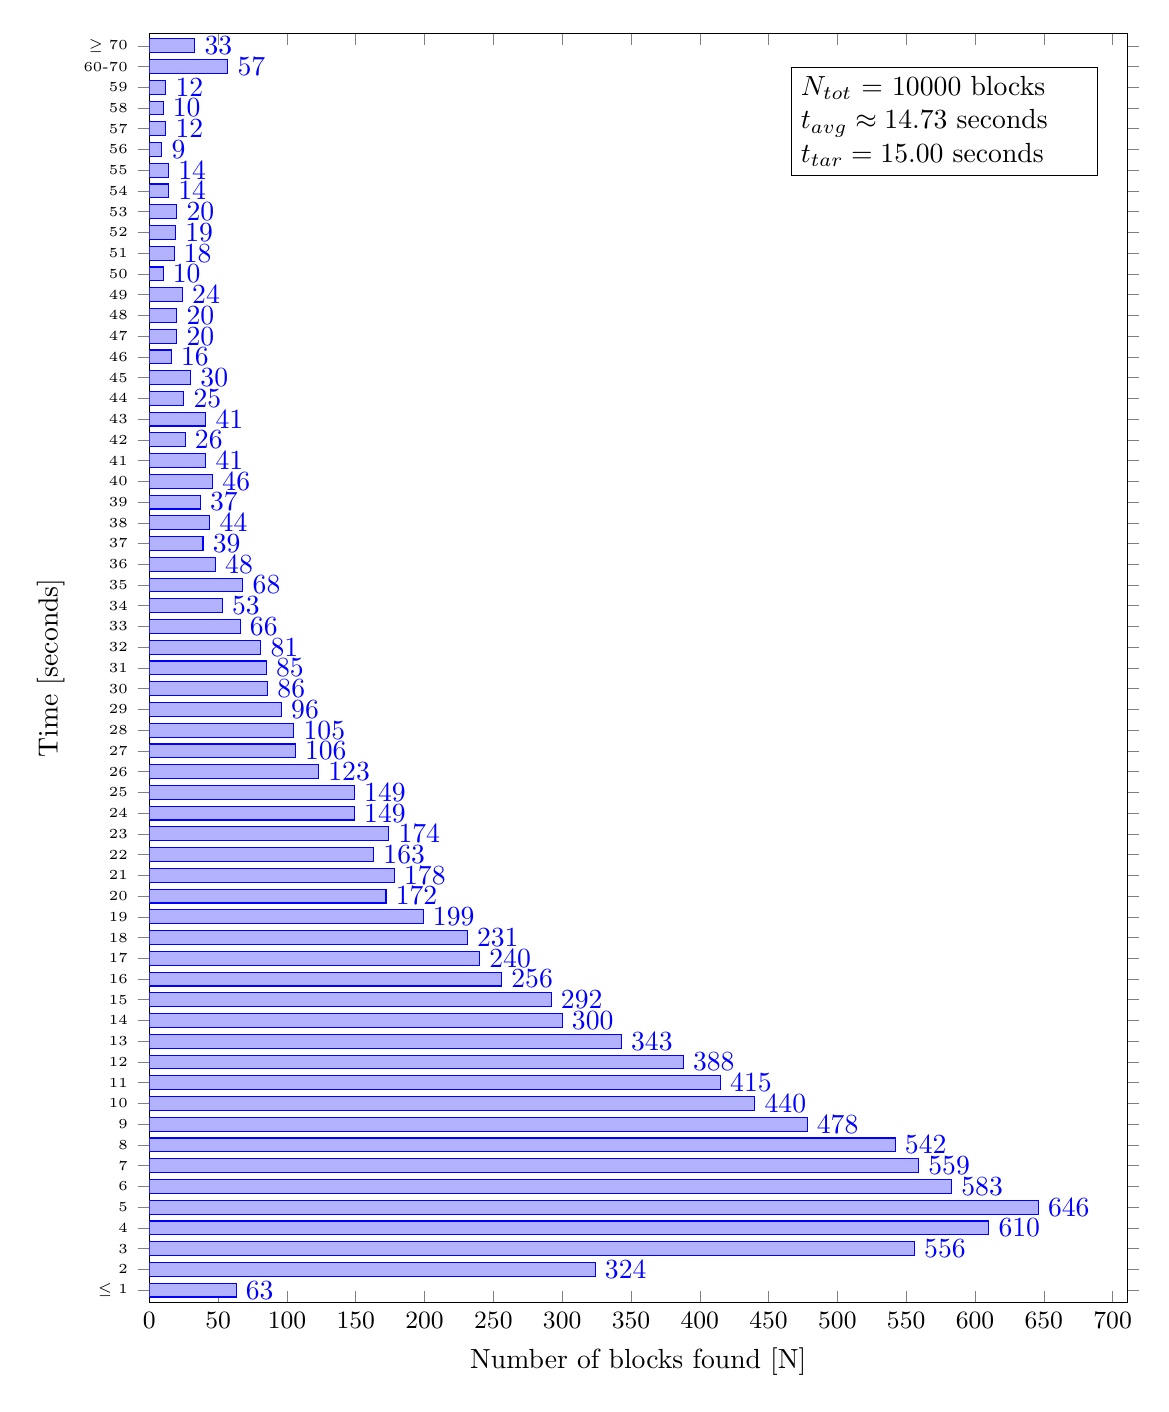
\begin{tikzpicture}
\node[draw, text width=3.65cm] at (10.1,15.0) 
    {$N_{tot}$ = 10000 blocks\\
    $t_{avg} \approx 14.73$ seconds\\
    $t_{tar} = 15.00$ seconds};
\begin{axis}[xbar,xmin=0,width=14cm, height=17.7cm, bar width=5pt,enlarge y limits=0.01,
y tick label style={font=\tiny},
x tick label style={font=\small},
xlabel={Number of blocks found [N]},
ylabel={Time [seconds]},
symbolic y coords={$\leq1$,2,3,4,5,6,7,8,9,10,11,12,13,14,15,16,17,18,19,20,21,22,23,24,25,26,27,28,29,30,31,32,33,34,35,36,37,38,39,40,41,42,43,44,45,46,47,48,49,50,51,52,53,54,55,56,57,58,59,60-70,$\geq70$},
ytick=data,
nodes near coords, nodes near coords align={horizontal},
]
\addplot coordinates {(63,$\leq1$) (324,2) (556,3) (610,4) (646,5) (583,6) (559,7) (542,8) (478,9) (440,10) (415,11) (388,12) (343,13) (300,14) (292,15) (256,16) (240,17) (231,18) (199,19) (172,20) (178,21) (163,22) (174,23) (149,24) (149,25) (123,26) (106,27) (105,28) (96,29) (86,30) (85,31) (81,32) (66,33) (53,34) (68,35) (48,36) (39,37) (44,38) (37,39) (46,40) (41,41) (26,42) (41,43) (25,44) (30,45) (16,46) (20,47) (20,48) (24,49) (10,50) (18,51) (19,52) (20,53) (14,54) (14,55) (9,56) (12,57) (10,58) (12,59) (57,60-70) (33,$\geq70$)};
\end{axis}
\end{tikzpicture}
\caption{Results of the Ethereum block time distribution test.}
\label{fig:ethtimetest}
\end{figure}

\pagebreak

\section{Visual representation of agreement states} \label{section:appendixdfa}

In Section \ref{section:statesofcontract}, a visual representation of the deterministic finite automaton $M$, which is shown in Figure \ref{fig:dfa}, was derived.

\begin{figure}[H]
\begin{center}
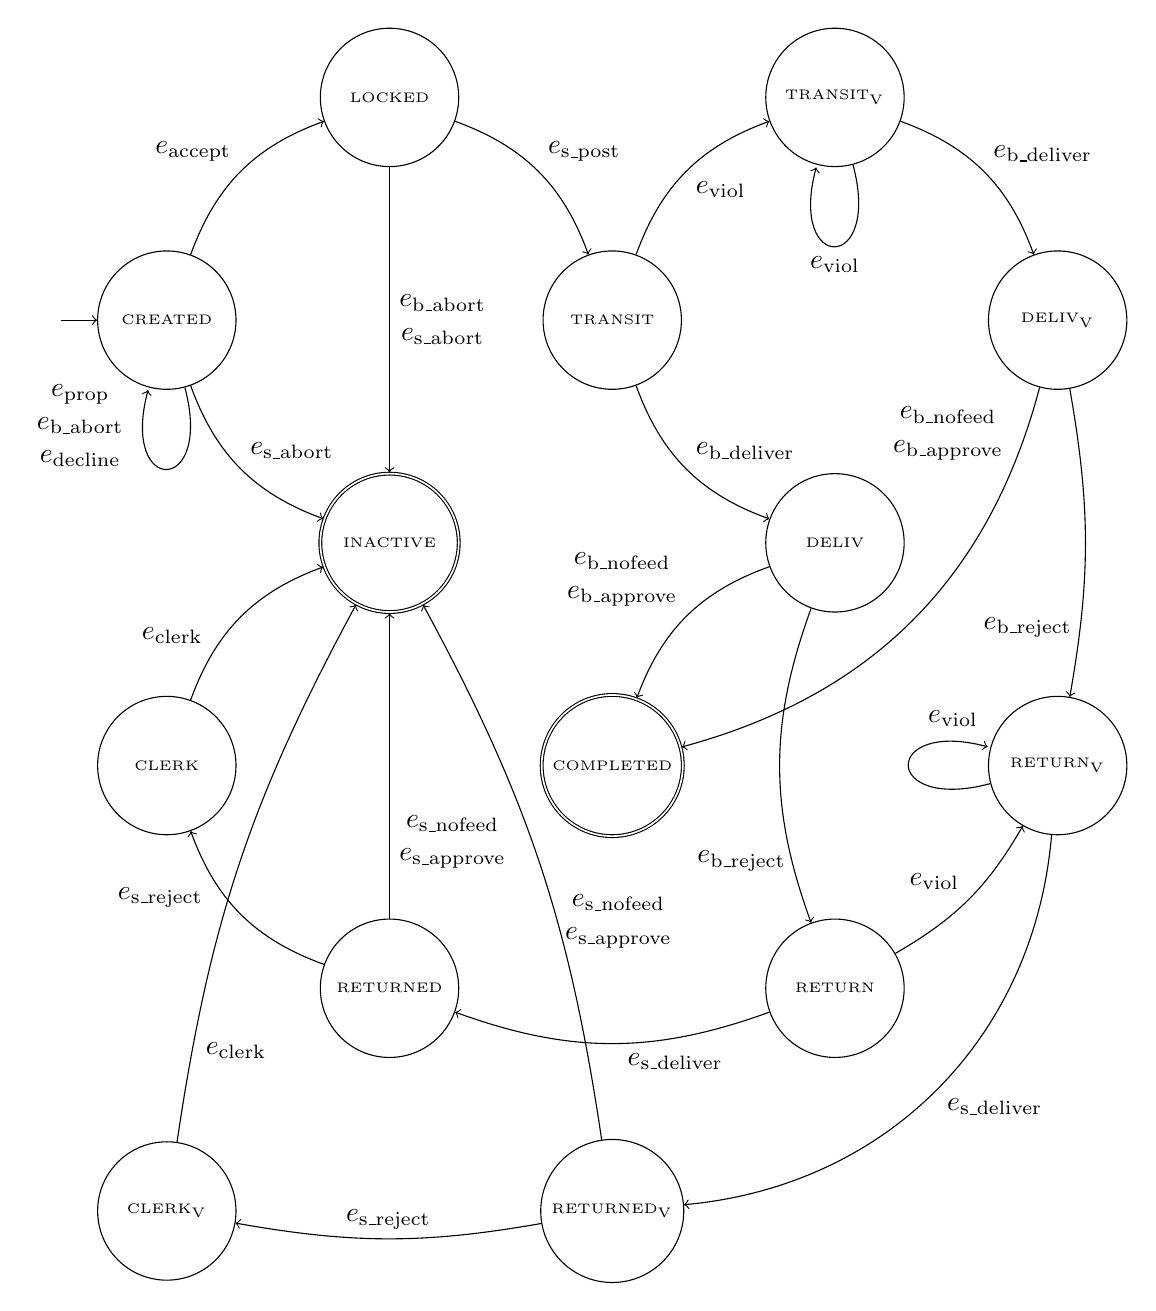
\begin{tikzpicture}[node distance=4cm,on grid,auto,initial text=, bend angle=25] 
   \node[state,initial,minimum size=5em] 		(CREATED)   							{{\tiny CREATED}}; 
   \node[state,minimum size=5em] 				(LOCKED)	[above right=of CREATED] 	{\tiny LOCKED};
   \node[state,accepting,minimum size=5em] 		(INACTIVE)	[below right=of CREATED] 	{\tiny INACTIVE};
   \node[state,minimum size=5em] 				(TRANSIT)	[below right=of LOCKED] 	{\tiny TRANSIT};
   \node[state,minimum size=5em] 				(TRANSITV)	[above right=of TRANSIT] 	{\tiny TRANSIT$_\mathrm{V}$};
   \node[state,minimum size=5em] 				(DELIV)		[below right=of TRANSIT] 	{\tiny DELIV};
   \node[state,minimum size=5em] 				(DELIVV)	[below right=of TRANSITV] 	{\tiny DELIV$_\mathrm{V}$};
   \node[state,accepting,minimum size=5em] 		(COMPLETED)	[below right=of INACTIVE] 	{\tiny COMPLETED};
   \node[state,minimum size=5em] 				(RETURNV)	[below right=of DELIV]	 	{\tiny RETURN$_\mathrm{V}$};
   \node[state,minimum size=5em] 				(RETURN)	[below right=of COMPLETED]	{\tiny RETURN};
   \node[state,minimum size=5em] 				(RETURNED)	[below left=of COMPLETED]	{\tiny RETURNED};
   \node[state,minimum size=5em] 				(RETURNEDV)	[below right=of RETURNED]	{\tiny RETURNED$_\mathrm{V}$};
   \node[state,minimum size=5em] 				(CLERKV)	[below left=of RETURNED]	{\tiny CLERK$_\mathrm{V}$};
   \node[state,minimum size=5em] 				(CLERK)		[below left=of INACTIVE]	{\tiny CLERK};
   
    \path[->] 
    (CREATED) 	edge [loop below] 		node[align=center,xshift=-11mm,yshift=12mm]					{$e_{\mathrm{prop}}$ \\ $e_{\mathrm{b\_abort}}$ \\ $ e_{\mathrm{decline}}$} 	()
    (CREATED) 	edge [bend left] 		node[align=center]											{$e_{\mathrm{accept}}$} 										(LOCKED)
    (CREATED) 	edge [bend right] 		node[align=center]											{$e_{\mathrm{s\_abort}}$} 									(INACTIVE)
    (LOCKED) 	edge			 		node[align=center]											{$e_{\mathrm{b\_abort}}$ \\ $e_{\mathrm{s\_abort}}$} 					(INACTIVE)
    (LOCKED) 	edge [bend left] 		node[align=center]											{$e_{\mathrm{s\_post}}$} 									(TRANSIT)
    (TRANSIT) 	edge [bend left] 		node[align=center,swap]										{$e_{\mathrm{viol}}$} 										(TRANSITV)
    (TRANSIT) 	edge [bend right] 		node[align=center]											{$e_{\mathrm{b\_deliver}}$} 									(DELIV)
    (TRANSITV) 	edge [loop below] 		node[align=center]											{$e_{\mathrm{viol}}$}										()
    (TRANSITV) 	edge [bend left] 		node[align=center]											{$e_{\mathrm{b\_deliver}}$}									(DELIVV)
    (DELIV) 	edge [bend right] 		node[align=center,swap]										{$e_{\mathrm{b\_nofeed}}$ \\ $e_{\mathrm{b\_approve}}$}				(COMPLETED)
    (DELIV) 	edge [bend right=20]	node[align=center,swap,near end,xshift=1mm]					{$e_{\mathrm{b\_reject}}$}									(RETURN)
    (DELIVV) 	edge [bend left=30] 	node[align=center,near start,swap,xshift=3mm,yshift=6mm]						{$e_{\mathrm{b\_nofeed}}$ \\ $e_{\mathrm{b\_approve}}$}				(COMPLETED)
    (DELIVV) 	edge [bend left=10] 	node[align=center,near end,swap,yshift=-4mm]				{$e_{\mathrm{b\_reject}}$}									(RETURNV)
    (RETURN) 	edge [bend right=15]		node[align=center]										{$e_{\mathrm{viol}}$}										(RETURNV)
    (RETURN) 	edge [bend left=20]		node[align=center,xshift=8mm]							{$e_{\mathrm{s\_deliver}}$}									(RETURNED)
    (RETURNV) 	edge [bend left=40]		node[align=center]											{$e_{\mathrm{s\_deliver}}$}									(RETURNEDV)
    (RETURNV) 	edge [loop left] 		node[align=center,xshift=10mm,yshift=6mm]					{$e_{\mathrm{viol}}$} 										()
    (RETURNED) 	edge [bend left]		node[align=center,near end]									{$e_{\mathrm{s\_reject}}$}									(CLERK)
    (RETURNED) 	edge					node[align=center,swap,near start]							{$e_{\mathrm{s\_nofeed}}$ \\ $e_{\mathrm{s\_approve}}$}				(INACTIVE)
    (RETURNEDV) edge [bend left=10]		node[align=center,swap]										{$e_{\mathrm{s\_reject}}$}									(CLERKV)
    (RETURNEDV) edge [bend right=10]	node[align=center,swap,xshift=2mm,yshift=-12mm]	{$e_{\mathrm{s\_nofeed}}$ \\ $e_{\mathrm{s\_approve}}$}	(INACTIVE)
    (CLERKV) 	edge [bend left=10]		node[align=center,near start,anchor=north west,xshift=-1mm,yshift=-5mm]	{$e_{\mathrm{clerk}}$}							(INACTIVE)
    (CLERK) 	edge [bend left]		node[align=center,near start]								{$e_{\mathrm{clerk}}$}										(INACTIVE);
\end{tikzpicture}
\caption{Visual representation of the deterministic finite automaton $M$.}
\label{fig:dfa}
\end{center}
\end{figure}

\pagebreak
\printbibliography[heading=bibintoc]

\end{document}
